\documentclass[12pt,english]{article}
\usepackage[T1]{fontenc}
\usepackage[latin9]{inputenc}
\usepackage[active]{srcltx}
\usepackage{enumerate}
\usepackage{amsthm}
\usepackage{amsmath}
\usepackage{amssymb}
\usepackage{graphicx}
\usepackage{setspace}
\usepackage{esint}
\usepackage[color=white,colorinlistoftodos]{todonotes}
% \usepackage[disable]{todonotes}
% \usepackage[draft]{todonotes}
\usepackage[round,longnamesfirst]{natbib}
\usepackage{lineno}
\usepackage{comment}

% Reference in letters
\usepackage{soul}
\usepackage{../utils/styles/qting}
\usepackage{xr}

% --- Preamble (once) ---
% \usepackage{booktabs}
% \usepackage{graphicx} % resizebox
% \usepackage{array}    % optional
\renewcommand{\arraystretch}{1.25} % taller rows (global)
% Preamble
\usepackage{booktabs}
\usepackage{threeparttable}
\usepackage{siunitx}
\usepackage{adjustbox}

\sisetup{
  table-number-alignment = center,
  table-text-alignment   = center,
  detect-weight          = true,
  detect-family          = true
}


% \usepackage{booktabs}
% \usepackage{array}
% \usepackage{threeparttable}
% \usepackage{adjustbox}   % for max width
% \usepackage{makecell}    % for manual line breaks in headers
% \renewcommand\theadfont{\bfseries}
% \renewcommand\arraystretch{1.15} % taller rows globally (or set locally below)

% \newcolumntype{C}[1]{>{\centering\arraybackslash}p{#1}}

\onehalfspacing

\definecolor{lightgray}{rgb}{1.0,0.0,0.0}

\bibliographystyle{aer}
\usepackage[titletoc,title]{appendix}

% \usepackage{subfigure}
\usepackage{subfiles}
\usepackage{subcaption}
\usepackage{rotating}
\usepackage{amsfonts}
\usepackage{caption}
\usepackage{placeins}
 		
\makeatletter
%%%%%%%%%%%%%%%%%%%%%%%%%%%%%% Textclass specific LaTeX commands.
  \theoremstyle{definition}
  \newtheorem{defn}{\protect\definitionname}
  \theoremstyle{plain}
  \newtheorem{prop}{\protect\propositionname}
  \theoremstyle{plain}
  \newtheorem{cor}{\protect\corollaryname}
  \theoremstyle{plain}
  \newtheorem{lem}{\protect\lemmaname}
 
%%%%%%%%%%%%%%%%%%%%%%%%%%%%%% User specified LaTeX commands.
\usepackage{booktabs}
\usepackage{threeparttable}
\usepackage{multirow}
\usepackage[margin=1in]{geometry}
\usepackage{relsize}
%\usepackage{setspace}
%\synctex = 1

 \usepackage[en-US]{datetime2}
\usepackage{mathtools}
\usepackage{xcolor}
\usepackage[thinlines]{easytable}
% \usepackage[table]{xcolor}

\newcommand{\comments}[1]
{\par {\bfseries \color{blue} #1 \par}}

\usepackage{todonotes}

 
% Environments  
\newtheorem{lemma}{Lemma}
\newtheorem{proposition}{Proposition}
\newtheorem{theorem}{Theorem}
\newtheorem{claim}[theorem]{Claim}
\newtheorem{corollary}{Corollary}
\newtheorem{definition}{Definition}
\newtheorem{example}{Example}
\newtheorem{assumption}{Assumption}
%\newtheorem{proposition}[theorem]{Proposition}
\newtheorem{remark}{Remark}
\newtheorem{problem}{Problem}
%\newenvironment{proof}[1][Proof]{\textbf{#1.} }{\  \rule{0.5em}{0.5em}}
 
\usepackage{amsmath}
\usepackage[bottom]{footmisc}
 
%\date{\normalsize \textcolor{webgreen}\\ Preliminary and Incomplete\\ Please do not circulate}
\usepackage{mathpazo}
%\usepackage{palatino}
 
%\usepackage{amsmath}
%\usepackage{amsfonts,amssymb}
%\usepackage[scale=.90]{lucimatx}
%\linespread{1.05}
 
%\usepackage[T1]{fontenc}
%\usepackage{textcomp}
%\renewcommand{\rmdefault}{ptm}
%\usepackage[scaled=0.92]{helvet}
%\usepackage[subscriptcorrection,nofontinfo,mtpcal,mtphrb,zswash]{mtpro2}
 
 
\renewcommand{\theenumi}{\roman{enumi}}
\usepackage{color}
\definecolor{webgreen}{rgb}{0,.5,0}
\definecolor{webbrown}{rgb}{.6,0,0}
\definecolor{webpurple}{rgb}{0.7,0,0.7}
 
%%%%%%%% hyperref stuff %%%%%%%%%%%%%%%%
\usepackage{hyperref}
\hypersetup{breaklinks = true,  
colorlinks=true, anchorcolor= webbrown, citecolor= webbrown,
filecolor= webbrown, linkcolor= webbrown, menucolor= webbrown,
urlcolor= webbrown, citebordercolor= 1 0 0, menubordercolor=1 0
0, urlbordercolor=1 0 0, runbordercolor=1 0 0 }
\usepackage{hypcap}
\hypersetup{pdfauthor=Nicolas Caramp}
%\hypersetup{pdfpagescrop={55 30 555 740}}
%%%%%%%%%%%%%%%%%%%%%%%%%%%%%%%%%%%%%%%%
 
%\DeclareMathOperator*{\plim}{plim}
 
%\tikzifexternalizing{%
        % do nothing in case 'true'
%}{%
        % ok, the main document is being generated:
%        \hypersetup{pdfpagescrop={55 30 555 740}}
%}
 
\newcommand{\tint}{\textstyle\int}
\newcommand{\tsum}{\textstyle\sum}
\usepackage{boxedminipage}
%\usepackage{appendix}
\usepackage[labelfont=bf]{caption}
 
 \newcommand{\paratitle}[1]{\vspace{1em}\noindent\textbf{#1}\hspace{1ex}}
 
 
%\usepackage{floatrow}
%\floatsetup[figure]{capposition=bottom,footposition=caption}
%\floatsetup[table]{objectset=justified}
%\captionsetup[figure]{footfont=small}
 
\makeatother
 
%\usepackage{babel}
  \providecommand{\definitionname}{Definition}
  \providecommand{\lemmaname}{Lemma}
  \providecommand{\propositionname}{Proposition}
\providecommand{\corollaryname}{Corollary}
% \input{setup.tex} % 

% \newpage

% \input{Letters.tex}

\newpage

\title{\textbf{Heterogeneous Beliefs, Asset Prices, \\and Business Cycles}\thanks{We are grateful for  helpful conversations with Andrew Atkeson, Sebastian Di Tella, Hamilton Gallardo, Fatih Guvenen, Fernando Mendo, Stavros Panageos, and Alp Simsek. We also thank three anonymous referees, the Central Bank of Chile, SED, and PUC-Rio participants, and the Santiago Macro Workshop 2019 for helpful comments. Bigio thanks the hospitality of the Federal Reserve Bank of San Francisco. We are indebted to Renata Avila for outstanding research assistance. All errors are ours.}
}
\author{ 
Saki Bigio\thanks{Department of Economics, UCLA, and NBER. E-mail: \href{sbigio@econ.ucla.edu}{sbigio@econ.ucla.edu}.} \and
Dejanir Silva\thanks{Mitch Daniels School of Business, Purdue University. E-mail: \href{dejanir@purdue.edu}{dejanir@purdue.edu}.}\and
Eduardo Zilberman\thanks{SPX Capital and Department of Economics, PUC-Rio. E-mail: \href{zilberman@econ.puc-rio.br}{zilberman@econ.puc-rio.br}.}}
\date{February 26, 2026}
% \date{\\
% 	\begin{small}
% 		First draft: May 5, 2018
% \end{small}}
\begin{document}
	\sloppy
	\maketitle
	\thispagestyle{empty}
	
\begin{abstract} 
	\noindent 
This paper develops a complete-market production economy with heterogeneous beliefs about TFP growth. 
Hiring occurs before TFP is known and is, therefore, risky (operating leverage). 
The firm's discount factor depends on a wealth-weighted average of investors' beliefs. 
Waves of optimism influence asset markets and percolate to labor hiring, tying together the equity premium, equity volatility, and labor volatility puzzles. 
A taxonomy of belief systems shows that only extrapolative beliefs amplify the volatility of asset prices and hours and lead to risk build up. 
Disciplined by survey data, the model matches asset-pricing and business-cycle moments, highlighting how heterogeneous beliefs can be a direct driver of aggregate fluctuations.
	\vspace{10mm}	
	\bigskip
	
	\noindent	
	\textsc{Keywords}: Heterogeneous Beliefs; Business Cycles; Asset Prices; Speculation.
	
	\medskip
	\noindent
	\textsc{JEL Classification}: D84, E32, E44, E71, G41.		
\end{abstract}

\newpage

\setcounter{page}{1}

\onehalfspacing

\newpage

\section{Introduction}
One of the oldest and most prominent economic narratives holds that swings in investor beliefs drive asset prices and business cycles. From \citet{sprague1910history} and \citet{fisher1933debt}, to \citet{keynes1936general}, \citet*{minsky1986stabilizing}, \citet*{kindleberger1996history}, and \citet*{Sh00}, a common theme emerges: fueled by leverage, a wave of excessive optimism drives up stock prices, spurring excessive firm investment and hiring. Once earnings disappoint, asset prices collapse on Wall Street with a blast wave felt all the way onto Main Street. Despite the prominence of this narrative, it remains unclear what ingredients theory needs to formalize these narratives in a quantitatively meaningful way.

We formalize these narratives in an otherwise frictionless economy. Markets are complete, prices are flexible, and there are no financial constraints. The only link between investor beliefs and output is that labor hiring is inherently risky: because employment must be chosen before productivity is realized, labor demand becomes a risky investment. The firm's discount factor---a wealth-weighted average of investor beliefs---dictates how this hiring risk is priced. When optimists grow wealthier, risk premia are compressed, and the firm discounts risk less aggressively, boosting labor demand. When this optimism is overcome by pessimism, the opposite occurs. Thus, waves of optimism on Wall Street indeed percolate onto Main Street.

Beyond formalizing the belief-driven business cycle narrative, the model yields sharp theoretical predictions. We derive an analytic taxonomy of belief systems that allows us to classify these systems according to their business-cycle amplification, risk build-up, and turnover properties. Moreover, disciplined by survey data on earnings expectations, belief heterogeneity accounts for these narratives in a quantitatively meaningful way. The model jointly matches:
\begin{enumerate}
    \item \textit{Asset-pricing and business-cycle moments.} The equity premium, stock-return volatility, and the volatility of hours worked---moments that are typically addressed in isolation but share a common origin in our setting: time-varying risk premia driven by shifts in the wealth distribution across investors.

    \item \textit{Excess volatility and return predictability.} Returns are more volatile than dividends, and the price-dividend ratio predicts future returns with a Campbell--Shiller discount-rate share close to unity, as in the data.

    \item \textit{Turnover dynamics.} Belief dispersion drives trading volume, and this relationship strengthens substantially in recessions---particularly around state transitions---consistent with patterns we document using I/B/E/S analyst forecasts and CRSP turnover data.

    \item \textit{Forecast biases in productivity expectations.} The model generates over-extrapolation in productivity growth forecasts, with a Coibion--Gorodnichenko coefficient that closely matches our estimates from the Survey of Professional Forecasters.
\end{enumerate}

\paragraph{The Model.} 
In the model, households differ in their beliefs about the evolution of TFP. Given their distinct views, they actively trade stocks, affecting asset prices. They supply labor with preferences that eliminate wealth effects, as in \citet[henceforth GHH]{GHH88}. 

The key feature is that heterogeneity in beliefs shapes the firm's labor demand because hiring is risky. As in \citet{burnside1993labor}, labor is chosen before the shock realizations. This timing induces an operating leverage channel whereby hiring becomes a risky investment, as it can add cost pressure to firms, which also occurs in labor search models.\footnote{We formally show that this form of \emph{investment in labor} is a simplified version of the investment in hours that happens in labor-search models.} This feature is critical to linking business-cycle fluctuations to asset-price fluctuations. We focus on the firm's investment in forming a workforce, as opposed to physical capital formation, because it is understood that, absent additional frictions, fluctuations in capital investment cannot be a source of business cycles; instead, what is needed are movements in the labor wedge \citep{CKM07}.\footnote{Investment is small relative to the capital stock in a business-cycle model. Thus, fluctuations in investment do not meaningfully impact the production possibility frontier.} Moreover, the operating leverage channel leads to testable implications regarding the correlation of returns and the labor share that is consistent with data, \citep[e.g., see][]{donangelo2019cross}.

Belief heterogeneity is essential for generating leverage and turnover dynamics, both recurrent themes in optimism-wave narratives. Because of heterogeneous beliefs, households take long or short positions in the firm. Optimistic households increase leverage, amplifying their risk exposure. Leverage creates internal propagation by magnifying differences in investors' risk exposures: optimistic investors accumulate relatively more wealth when positive shocks occur, while pessimists gain during downturns.

These dynamics produce internal propagation as wealth-weighted beliefs jointly affect asset prices and output through the operating leverage channel. When wealth-weighted beliefs become more optimistic, increased demand for risky assets pushes stock prices upward, compresses risk premia, and encourages hiring. Thus, as investors' risk appetite increases, discount rates decline, prompting more hiring by a firm attempting to raise its market value. Through these dynamics, the \emph{equity premium}, the \emph{equity volatility}, and \emph{labor volatility} puzzles are tied together into a single volatility puzzle. 

\paragraph{Theoretical Results.} Despite featuring Epstein-Zin preferences and endogenous labor supply, the model remains highly tractable due to a convenient ``as if'' property portable to other settings. Specifically, the equilibrium is characterized as if the economy were an endowment economy, with a common stochastic discount factor (SDF) used to price assets. Importantly, the firm makes risky hiring decisions using a common SDF. To increase the firm's value, it constructs a risk-neutral productivity growth expectation consistent with the SDF. This risk-neutral expectation ultimately determines employment. Crucially, we impose no assumptions regarding the firm's direct knowledge of investor beliefs; the firm only needs to understand how its hiring decisions affect its market value. 

In the special case of log utility, the model admits an analytic solution, enabling us to articulate a clear taxonomy of belief systems. \q{ResultSummary}{Specifically, we classify beliefs into two broad categories, each with two sub-categories. The first category comprises \emph{rank-preserving} beliefs, subdivided into optimistic and pessimistic beliefs. The second category includes \emph{rank-alternating} beliefs, subdivided into extrapolative and intrapolative beliefs. This taxonomy allows us to derive general properties regarding how each belief structure affects business-cycle dynamics.

We identify several principles regarding the amplification properties under different belief systems. First, we show that only extrapolative beliefs amplify business-cycle fluctuations across all states of the economy relative to rational expectations. Amplification occurs because extrapolation boosts the firm's discounting of risk states during booms but depresses it during busts, a property unique to extrapolative beliefs.

Second, we uncover that only extrapolative beliefs engender \textit{risk build-up}, i.e., longer booms lead to deeper busts. This phenomenon, also exclusive to extrapolative belief systems, occurs because extrapolative households consistently accumulate wealth throughout boom phases. When the economy transitions into a downturn, extrapolative agents remain wealthier while simultaneously becoming the most pessimistic investors. The reversal in the wealthiest households' optimism significantly amplifies the economy's rift.}

Third, we demonstrate that belief heterogeneity drives stock turnover through two first-order forces: by inducing passive rebalancing as differences in beliefs translate into differences in wealth growth rates within states and by the changes in beliefs when the economy changes states. We further show that when beliefs are rank-alternating, turnover increases most when the economy enters a recession, a property that we verify in the data.

Our taxonomy highlights the importance of belief heterogeneity for understanding macro-finance dynamics. Empirical evidence from \citet{lopez2017credit} and \citet{krishnamurthy2017credit} indicates that risk premia are low during credit booms preceding severe crashes.\footnote{See also \citet{gennaioli2018crisis} and \citet{krishnamurthy2025dissecting}.
} In contrast, standard macro-finance models without belief heterogeneity predict precisely the opposite  \citep[e.g.,][]{brunnermeier2014macroeconomic,he2013intermediary}.
Furthermore, our analysis helps distinguish models driven by heterogeneous beliefs from those driven by heterogeneous risk aversion \citep[e.g.,][]{panageas2020implications}, a challenge for the literature. Our results clarify that heterogeneity in risk aversion cannot generate risk build-up germane to extrapolative belief systems. 

\paragraph{Quantitative Results.}
To complement our theoretical insights, we provide a quantitative evaluation. Aside from beliefs, our framework follows canonical assumptions; we adopt a standard calibration approach for preferences and the process for TFP. To discipline the calibration of beliefs, we utilize survey data on earnings forecasts. The belief process is parsimonious: two key parameters---an overreaction coefficient and the volatility of a sentiment shock---are pinned down by the degree of return extrapolation observed in surveys and the excess volatility of survey-based expectations relative to realized outcomes. This specification nests the belief systems identified in our taxonomy, so we let the data determine whether the empirically relevant system is extrapolative, rank-preserving, or a combination.

Our quantitative analysis underscores the importance of each ingredient by following a progression. Operating leverage alone matches dividend-growth volatility but fails on equity returns and employment. Homogeneous subjective beliefs add labor fluctuations but cannot generate a realistic equity premium. Only the interaction of rational and extrapolative investors---and the wealth dynamics it produces---allows the model to jointly match the moments listed above.

\paragraph{Literature Review.}

This paper connects to the literature initiated by \citet{KP82} and \citet{MP85}, who used complete-market benchmarks to analyze business cycle fluctuations and asset prices in settings where these two dimensions do not feed into each other. A recent strand emphasizes the role of fluctuating risk premia in driving real cycles, particularly highlighting the riskiness of labor hiring \citep[e.g.,][]{H17, BB19, DH19, KLMP19}. We bridge this channel with the literature on heterogeneous beliefs and asset pricing.

\citet{HK78} and \citet{SX03} formalized how heterogeneous beliefs induce asset-market trade, emphasizing that belief heterogeneity engenders asset-price volatility through leverage. A virtue of these formalizations is their subtle departure from strict rational expectations: agents fully understand the structure of the economy and the risks it entails, yet disagree about the distribution of future fundamentals. Investors can therefore hold different views about which firms or technologies are more likely to succeed, while recognizing the risks inherent in taking positions on those outcomes. Importantly, a modeler is not free to impose arbitrary beliefs about asset prices onto agents whose decisions determine those very prices. We embrace this approach. 

Building on those foundations, a large body of work examines how belief heterogeneity interacts with financial constraints to generate speculative bubbles \citep[e.g.,][]{G03, FG08, G10, S13, INS18, barlevy2014leverage, barlevy2022speculative}, while closely related papers explore how wealth redistribution driven by heterogeneous beliefs affects asset-price dynamics \citep{DM94, XY09, KS12, wr2022sentiment}. This earlier literature set aside the connection to the real economy. We view our paper as a natural progression of these models, linking belief heterogeneity to the real economy through the labor market.

A growing body of macro-finance work embeds beliefs into environments where these affect production, but optimism affects output by interacting with market imperfections such as incomplete markets, financial frictions, or demand externalities. Some models connect speculative bubbles to real activity through capital investment,\footnote{See \cite{GHH05}, \cite{BSX06}, \cite{P05}, and \cite{BDUV16}.} while others explore how heterogeneous beliefs interact with aggregate demand externalities, highlighting how changes in wealth distribution can amplify demand-driven recessions \citep{CS19, CS20, guerreiro2022disagreement, CS24}. \citet{simsek2021macroeconomics} provides a comprehensive review.

Our paper fills a gap between these two literatures: models where belief heterogeneity drives asset prices but has no impact on the real economy, and models where beliefs affect output only by aggravating market imperfections. To our knowledge, there is no frictionless benchmark economy where belief heterogeneity is a source of business-cycle fluctuations in its own right. Developing such a benchmark is important: First, by abstracting away market imperfections, we can provide a qualitative and quantitative assessment of the direct effects of beliefs on the business cycle. Second, we can uncover general principles that carry over to environments with market imperfections. Finally, a frictionless benchmark serves as an ideal target that policy interventions to mitigate market imperfections should strive to replicate. After all, policy should not care about asset prices per se, but only inasmuch as these create inefficiencies.

Our theoretical results emphasize that extrapolative beliefs conform best with the narratives and empirical patterns documented above, providing a disciplined rationale for their prominence in the literature. This connects us to models featuring diagnostic expectations \citep{GS10, bianchi2024diagnostic} and, more broadly, to the literature on subjective beliefs and macroeconomic dynamics \citep[e.g.,][]{EP11, ACD18, BGS18, BBH19}. Most closely related, \cite{AM19} shows how extrapolative beliefs simultaneously explain stock market and business cycle fluctuations, but in a setting with homogeneous beliefs. Our taxonomy clarifies that heterogeneity is essential for generating risk build-up and the turnover dynamics that are central to optimism-wave narratives.

Finally, our model generates sharp predictions for trading volume, a dimension that receives surprisingly little attention in equilibrium asset-pricing models.\footnote{\citet{AlvarezAtkeson2018} develop a general equilibrium model where trade volume becomes a pricing factor through idiosyncratic shocks to risk tolerance.} On the empirical side, \citet{vanderBeck2025} show that the ratio of return volatility to portfolio turnover provides a lower bound on price impact that is tightened by disagreement, establishing that trading activity is central to understanding asset price movements. \citet{ThesmarVerner2025} and \citet{McCarthyHillenbrand2025} independently document that disagreement between sophisticated and extrapolative investors is associated with higher trading volume and accounts for a large share of stock price variation. Our model complements these findings with a structural foundation for these findings, linking disagreement to turnover, asset prices, and employment within a unified framework.

\paragraph{Roadmap.} The next section presents three empirical facts about investor beliefs documented in the literature to motivate our analysis. Subsequently, we present the theoretical model followed by the quantitative evaluation. Finally, we conclude.

\section{Three motivating facts}
\label{sec:facts.sec}

This section discusses three facts about subjective expectations that motivate our model. 

\paragraph{Fact 1. Expectations are volatile.}
As \citet{shiller1981stock} famously observed, stock dividends and earnings are too stable to explain the large swings in asset prices. In contrast, recent survey evidence shows that \textit{subjective expectations} of future cash flows are highly volatile, offering a potential explanation for the stock market's excess volatility \citep{bordalo2020expectations, de_la_o_subjective_2021}.

We illustrate the magnitude of the difference in the volatility of subjective and objective expectations by constructing an "objective" forecast---based on the statistical properties of dividends---against a survey-based "subjective" forecast. Specifically, we estimate an AR(1) process for quarterly aggregate dividend and earnings growth. The predicted one-year-ahead dividend growth from this AR(1) serves as our measure of objective expectations, $\mathbb{E}^{obj}[\Delta d_{t,t+4}]$. We then compute the fraction of the total variance in realized dividend growth expectations relative to the variance of realized dividend growth. We construct an analogous measure for subjective expectations, $\mathbb{E}^{sub}[\Delta d_{t,t+4}]$, by using the survey of analyst expectations from I/B/E/S. The differences in volatility are significant:
\begin{equation}
    \frac{\mathrm{Var}\!\bigl[\mathbb{E}^{obj}[\Delta d_{t,t+4}]\bigr]}{\mathrm{Var}[\Delta d_{t,t+4}]} = 0.05,
    \qquad\quad
    \frac{\mathrm{Var}\!\bigl[\mathbb{E}^{sub}[\Delta d_{t,t+4}]\bigr]}{\mathrm{Var}[\Delta d_{t,t+4}]} = 0.70.
    \nonumber
\end{equation}
Whereas objective expectations represent a negligible fraction of the total variation in dividend growth, subjective expectations are an order of magnitude more volatile.\footnote{The small fraction of variation explained by objective expectations is consistent with the estimated autocorrelation of cash flows in, for example, \citet{bansal2004risks}.}

% Next, we provide a sense of the importance of belief heterogeneity, we investigate the link between investor heterogeneity and  turnover volume. Turnover is informative about the importance of our mechanism: if investors forecast errors are random across agents and time, stock turnover should be zero and thus, a model with homogeneous beliefs should be a good representation of reality. In turn, if a set of investors is rational turnover should also be zero. If turnover and market returns are correlated, this is evidence of belief heterogeneity.

% This discussion motivates our model. With a model, we can then provide an explicit relation between belief heterogeneity and stock market turnover to better approximate the importance of belief heterogeneity in explaining asset prices.  

% we argued that there is some inconsistency in the volatility predicted by DLM. I forgot what it was, but I'm wondering if we can use some convex combination: $\mathbb{E}_{t}^{m}=\beta*\mathbb{E}_{t}^{i}+(1-\beta)*\mathbb{E}_{s}^{i}$ to be estimated (estimate beta) and then argue they matter.

\paragraph{Fact 2. Expectations are heterogeneous.}
Fact 1 provides evidence of deviations from full-information rational expectations (FIRE). 
Our business cycle model emphasizes how heterogeneity in these expectations leads to business cycle amplification through asset markets. 
Critical to our theory is the presence of heterogeneity in beliefs. 
Concrete evidence is surveyed in \citet{nagel2023dynamics} reporting subjective return expectations across individual investors, CFOs, and professional forecasters. 
Table~\ref{tab:nx_regression} summarizes their findings: The first column shows that realized future returns are positively predicted by the dividend-price ratio (a standard return predictor). 
In contrast, past returns do not appear significantly. 
In contrast, regressions for subjective expected returns reveal heterogeneous beliefs: individual investors place a positive and significant weight on past returns (consistent with extrapolation), professional forecasters behave in a contrarian way (a negative coefficient on past returns indicates interpolation), and CFOs lie somewhere in between. 
These results underscore the importance of heterogeneity in expectations among different agents.\footnote{
    See also \citet{atmaz2023contrarians} for evidence of both extrapolative and contrarian behavior. 
    \citet{greenwood_expectations_2014} provides further evidence of extrapolative expectations from past stock return, also associated with the cyclicality of credit and leverage \citep{lopez2017credit}.} 

\begin{table}[t!]
    \centering
    \caption{Subjective return expectations regressions by type of investor.}
    \label{tab:nx_regression}
    \begin{tabular}{lcccc}
   \midrule \midrule
   Dependent var.:         & \textbf{Objective}           & \textbf{Individual}            & \textbf{CFO}            & \textbf{Professional}\\  
   \midrule
   \emph{Predictors}\\
   D/P            & 5.83   &  -0.00  & -0.41  & 0.42\\   
    \hspace{0.2cm}\small{(p-value)} & (0.00) &  (1.00) & (0.31) & (0.73)\\   
   $R_{past}^e$   & 0.36   &  0.87   & 0.30   & -2.78\\   
    \hspace{0.2cm}\small{(p-value)} & (0.71) & (0.02)  & (0.29) & (0.01)\\   
   \midrule \midrule
\end{tabular}
\end{table}


For our paper, a key question is whether expectations correlate with actual trading behavior. 
Existing evidence suggests that yes: \citet{greenwood_expectations_2014} shows that subjective expectations correlate with mutual fund flows, and \citet{GMSU_AER} documents a relationship between beliefs and portfolio choices.\footnote{
    In Section~\ref{sec:belief_taxonomy.sec}, we construct a measure of heterogeneity among professional forecasters and show that this measure of disagreement correlates with stock market turnover, particularly during recessions.}

\paragraph{Fact 3. Expectations correlate with hiring decisions.}

% Previous Table 2 (kept for record; commented out)
% \begin{table}[h!]
% \centering
% \caption{I/B/E/S Expectations and Labor}
% \scalebox{0.9}{
% \begin{tabular}[t]{lcccccc}
%  \tabularnewline \midrule \midrule
%    Dependent Variable: & \multicolumn{3}{c}{$Payroll$} & \multicolumn{3}{c}{Number of workers}\\
%    Model:     & (1) & (2) & (3) & (4) & (5) & (6) \\
%    \midrule
% (Intercept)      & 0.388     & 0.274     & 0.364 & 0.392 & 0.143 & 0.170\\
%                     & (0.247)   & (0.223)   & (0.241) & (0.097) & (0.195) & (0.052)\\
% lag earning growth expectation         & 0.133*** & 0.135*** & 0.136*** & 0.061*** & 0.062*** & 0.067***\\
%                    & (0.043)    & (0.043)   & (0.043)  & (0.014) & (0.014) & (0.014)\\
% 12-month lag return &  & 0.474*** &  &  & 0.535*** & \\
% 		&  & (0.119) & &  & (0.054) &\\
% 12-month return &  &  & 0.234* &  &  & 0.326*** \\
%  			&   &  & (0.125)  &  &  & (0.043) \\
%      \midrule
%      \emph{Fit statistics}\\
% Observations      & 1797  & 1797 & 1797 & 1797  & 1797 & 1797\\
% R2                       & 0.081 & 0.090 & 0.083 & 0.081 & 0.090 & 0.083 \\
% Adjusted R2        & 0.038 & 0.046 & 0.039 & 0.038 & 0.046 & 0.039 \\
%   \midrule \midrule
%    \multicolumn{4}{l}{\emph{Newey-West standard-errors in parentheses (4 lags)}}\\
%    \multicolumn{4}{l}{\emph{Signif. Codes: ***: 0.01, **: 0.05, *: 0.1}}\\
%
% \hline \\[-1.8ex]
% \end{tabular}}
%  \label{tab:payroll}
% \end{table}

\begin{table}[t]
\centering
\caption{I/B/E/S Expectations and Labor}
\label{tab:payroll}
\small
\begin{tabular}{lcccccc}
\toprule\toprule
Dependent Variable: & \multicolumn{3}{c}{Payroll} & \multicolumn{3}{c}{Number of workers} \\
Model: & (1) & (2) & (3) & (4) & (5) & (6) \\
\midrule
(Intercept) & 0.491*** & 0.456*** & 0.467*** & 0.177*** & 0.129*** & 0.158*** \\
 & (0.035) & (0.037) & (0.038) & (0.033) & (0.036) & (0.033) \\
Lag earning growth expectation & 0.230*** & 0.187*** & 0.228*** & 0.277*** & 0.219*** & 0.276*** \\
 & (0.037) & (0.038) & (0.036) & (0.070) & (0.078) & (0.070) \\
12-month lag return &  & 0.326*** &  &  & 0.443*** &  \\
 &  & (0.084) &  &  & (0.101) &  \\
12-month return &  &  & 0.178** &  &  & 0.134 \\
 &  &  & (0.079) &  &  & (0.097) \\
\midrule
\emph{Fit statistics} \\
Observations & 1,746 & 1,746 & 1,746 & 1,746 & 1,746 & 1,746 \\
$R^2$ & 0.036 & 0.044 & 0.039 & 0.036 & 0.047 & 0.037 \\
% Adjusted $R^2$ & 0.035 & 0.043 & 0.038 & 0.036 & 0.046 & 0.036 \\
\midrule\midrule
\multicolumn{7}{l}{\emph{Standard errors clustered at the firm level in parentheses.}} \\
\multicolumn{7}{l}{\emph{Significance: *** $p<0.01$, ** $p<0.05$, * $p<0.10$.}} \\
\bottomrule
\end{tabular}
\end{table}


The previous two facts focus on \emph{subjective expectations} among groups of investors. Toward a business cycle theory, a natural follow-up question is whether these expectations are reflected in \emph{real} economic outcomes. Indeed, \citet{GMS16} shows that CFO expectations predict corporate capital investment, and \citet{armona2019home} finds that expectations about home price appreciations influence construction. In this spirit, we present related evidence: investor expectations also predict firm-level \emph{employment} decisions. To demonstrate this, we use two labor-related measures from Compustat Annual: the realized growth in staff expenses (payroll) and the employee count (workers). These two measures are standardized using the same procedure we apply to our earnings data.

\q{GennaioliStyleRegression}{
We follow the approach of \citet{GMS16}: we regress realized employment growth on the firm-level earnings growth expectations drawn from I/B/E/S. We control for past 12-month stock returns (constructed using individual stock prices from CRSP) and contemporaneous returns, clustering standard errors at the firm level. By including past returns, we aim to capture systematic shocks that might otherwise confound the relationship between expectations and subsequent employment growth.

Table \ref{tab:payroll} shows that earnings growth expectations predict realized employment growth in both total payroll and the number of workers. In light of Facts 1 and 2---namely, that earnings growth expectations exhibit greater volatility than actual outcomes and that CFOs behave differently from individual investors---these results provide reassuring evidence that firm employment decisions correlate with investor expectations.
}

\q{GennaioliCaveat}{
Naturally, this correlation alone does not establish causality: it may simply reflect that the surveyed analysts' information overlaps with managers' private signals, even if investors do not directly influence managers. However, \citet{GMS16} finds that investor expectations continue to affect capital investment even after controlling for managers' survey responses, suggesting a meaningful role for such external perceptions. Unlike \citet{GMS16}, we cannot control for CFO expectations, as we lack sufficient data matches for the employment variables. Motivated by the three facts, we proceed to the model.
}

\section{Model}\label{sec:environment.sec}

 We consider a two-state complete-markets economy with time indexed by $t\in\{0,1,...,\}$. The economy is populated by heterogeneous households that differ in their beliefs regarding TFP growth. Households hold (or issue) risk-free bonds and hold (or short-sell) shares of a single representative firm. Differences in beliefs induce a desire to lever up. 
The firm hires labor one period in advance before TFP is realized. Hiring in advance links labor demand with asset pricing.

\paragraph{The exogenous state.}
Total factor productivity $A_{t}$ grows according to a two-state Markov process:
\begin{equation}
    \frac{A_{t+1}}{A_t} = x_{t+1},
\end{equation}
where $x_{t+1} \in \{x_L, x_H\}$, $0<x_L <x_H $. Transition probabilities from state $s$ to $s'$ are denoted by $\{p_{ss'}\}$. 

\paragraph{The firm.}
The representative firm produces a final good according to $A_{t+1} h_{t+1}^\alpha$, where labor $h_{t+1}$ is hired in period $t$, prior to the realization of $x_{t+1}$. While firms hire and contract the wage $W_{t+1}$ one period ahead, the wage bill is paid when production is finished.

The firm takes hours at the initial date $h_0$ as given and hires labor in subsequent periods to maximize its value using a stochastic discount factor (SDF), $\Lambda_{t,t+1}$: 
\begin{equation} \label{eq: firm_value}
    Q_t =\max_{h_{t+1}}  \mathbb{E}_t\left[ \Lambda_{t,t+1} \left(\pi_{t+1} + Q_{t+1} \right)\right].
\end{equation}
$Q_t$ denotes the firm value and $\pi_{t+1} \equiv A_{t+1} h_{t+1}^\alpha -W_{t+1} h_{t+1}$ denotes the profit (dividend). 
Expectations are taken with respect to the transition probabilities $\{p_{ss'}\}$. 
Because markets are complete, there is a unique SDF for any fixed set of beliefs. 
Hence, there is unanimity regarding the firm's objective among shareholders, as discussed in  Section \ref{subsec:investors_problem}. 
Beliefs affect employment decisions through their impact on the SDF.

\paragraph{Households.}
There is a finite number of infinite-lived households, indexed by $i \in \mathcal{I}= \{1, \ldots, I\}$ with masses $\{\mu_i\}$, $\sum_i \mu_i = 1$. Household $i$ derives utility from consumption $C_{i,t}$ and disutility from working $h_{i,t}$. They have Epstein-Zin preferences over a GHH consumption-labor composite:
\begin{equation}\label{eq: preferences}
    V_{i,t} = (1-\beta) U\left(C_{i,t} - \xi_t \frac{h_{i,t}^{1+\nu}}{1+\nu}\right) + \beta U\left( \mathcal{V}_{i,t} \right),
\end{equation}
where $V_{i,t}$ denotes the utility level, $\beta$ the discount factor, and $\xi_t$ controls the labor disutility. $\mathcal{V}_{i,t}$ is the certainty-equivalent of future utility, $\mathcal{V}_{i,t} = \Psi^ {-1}\left( \mathbb{E}_{i,t}\left[ \Psi\left( U^ {-1}(V_{i,t+1}\right)\right] \right)$.

The labor disutility coefficient is indexed by \textit{lagged} productivity, $\xi_{t} = \xi A_{t-1}$ and acts as a long-run wealth effect---as in \citet{JR09}, this ensures that hours are stationary. 
We adopt the functional forms: $U(C) = \frac{C^{1-1/\psi}-1}{1-1/\psi}$ and $\Psi(Z) = \frac{Z^{1-\gamma} -1}{1-\gamma}$, where $\gamma$ controls risk aversion and $\psi$ the elasticity of intertemporal substitution $(EIS)$.\footnote{CRRA preferences correspond to $\psi = \gamma^{-1}$.
Given the endogenous labor supply, $\gamma$ controls but does not coincide with the risk aversion for lotteries on financial wealth (see, e.g., \citealt{swanson2018risk}).
} As $U(\cdot)$ is defined over positive values, \textit{net consumption}, $C_{i,t} - \xi_t \frac{h_{i,t}^{1+\nu}}{1+\nu}$, must be positive.

Household $i$ has beliefs $\{p^i_{ss'}\}$ regarding TFP growth $x_{t+1}$ from state $s$ to $s'$ and forms an expectation $\mathbb{E}_{i,t}$ accordingly. Households are dogmatic, as in \citet{chen2012rare} and \citet{simsek2013speculation}: they \textit{agree to disagree} and do not learn from the views of others. 
Beliefs about productivity translate into beliefs about earnings and asset prices.

Household $i$ chooses consumption $C_{i,t}$, hours $h_{i,t}$, firm shares $S_{i,t}$, and risk-free bonds $B_{i,t}$ to maximize \eqref{eq: preferences} subject to a flow budget constraint
\begin{equation}\label{eq: flow_bc}
    C_{i,t} + Q_t S_{i,t} + B_{i,t} = R_{r,t} Q_{t-1} S_{i,t-1} + R_{f,t-1} B_{i,t-1} + W_t h_{i,t}.
\end{equation}
We denote human wealth by:
\begin{equation}\label{eq: human_wealth}
   \mathcal{H}_{i,t} = \mathbb{E}_t\left[ \sum_{k=1}^\infty \Lambda_{t,t+k} \left( W_{t+k} h_{i,t+k}- \xi_{t+k} \frac{h_{i,t+k}^{1+\nu}}{1+\nu}  \right) \right].
\end{equation}
Human wealth is the present discounted value of future \textit{net labor income}. 
Net labor income equals the labor earnings minus labor disutility. The present value is discounted using the SDF $\Lambda_{t,t+k} = \prod_{j=1}^k \Lambda_{t+j-1,t+j}$. 
The SDF is the same as the one used to value firms. 

Households face a natural borrowing limit: $R_{r,t}Q_{t-1} S_{i,t-1} + R_{f,t-1} B_{i,t-1} + W_t h_{i,t}- \xi_t \frac{h_{i,t}^{1+\nu}}{1+\nu} \geq -\mathcal{H}_{i,t}$, given $S_{i,-1}$ and $B_{i,-1}$, where $R_{f,t}$ denotes the return on the risk-free bond and $R_{r,t} = \frac{Q_t + \pi_t}{Q_{t-1}}$ the return on stocks, the risky asset in this economy.\footnote{This borrowing limit corresponds to the maximum households can borrow without violating the non-negativity of net consumption and is therefore never binding in equilibrium.}

\paragraph{Example I: Diagnostic expectations.} 
We do not impose restrictions on beliefs. 
In particular, our formulation is flexible enough to capture different belief dynamics, including extrapolation or underreaction. 
For example, consider the case of \textit{heterogeneous diagnostic expectations}. 
\q{DE_definition}{Diagnostic expectations correspond to the following belief structure:\footnote{
    Diagnostic expectations are defined using distorted probabilities of the form
$\Pr^i(T=t\mid G)\propto \Pr(T=t\mid G)\left(\frac{\Pr(T=t\mid G)}{\Pr(T=t\mid -G)}\right)^{\theta_i}$
(see, e.g., \citealt{bordalo2018diagnostic}).
In our setting, the trait $T$ is next period's state $s'$, the group $G$ is the current
state $s$, and the reference group $-G$ is the alternative state $-s$.
}
\begin{equation}
    p_{sH}^i = \underbrace{p_{sH}}_{\text{rational beliefs}} \times \underbrace{\left( \frac{p_{sH}}{p_{-sH}} \right)^{\theta_i}}_{\text{belief distortion}} \times C,\nonumber
\end{equation}}
where $C$ is a normalizing constant, $p_{sH}$ and $p_{-sH}$ denote the probability of being in the high state next period if the current state is $s$ and not $s$, respectively, and $\theta_i$ is a parameter controlling diagnosticity.
If productivity growth is persistent under rational beliefs, i.e., $p_{HH} > p_{LH}$, then under diagnostic expectations, households overreact to news: households believe it is more likely they would remain in the high (low) state after switching to the high (low) state.
If $p_{ss} = \frac{1+\rho}{2}$, as in \citet{MP85}, then $p_{ss}^i = \frac{1+\rho_i}{2}$,  where $\rho_i > \rho$, and the (endogenous) subjective persistence parameter $\rho_i$ is a function of $\theta_i$.

\paragraph{Example II: Optimism and pessimism.}  Diagnostic expectations capture a form of extrapolation: households are optimistic in the boom and pessimistic in the bust. 
Alternatively, we could have a persistent degree of optimism/pessimism: $ p_{sH}^i = p_{sH} + \Delta_i$
where households with $\Delta_i > 0$ would be optimistic at all states.

Both the diagnostic expectations and persistent optimism formulations are one-parameter belief specifications. 
In general, beliefs can depend on two parameters, capturing a combination of these two cases: $ p_{HH}^i = (1+\rho_i)/2+\Delta_i$ and $p_{LL}^i = (1+\rho_i)/2 -\Delta_i.$\footnote{Notice that diagnostic beliefs coincide with rational beliefs in the case productivity growth is iid, $p_{sH} = p_{-sH}$. 
Our formulation allows for an arbitrary persistence under subjective beliefs, even in this case.
}

\paragraph{SDF and equilibrium.}

\q{SDF_inference}{
The SDF can be inferred from the process of asset returns through no-arbitrage conditions:
\begin{equation}\label{eq: no_arbitrage}
    1 = \mathbb{E}_t\left[ \Lambda_{t,t+1} \frac{\pi_{t+1}+Q_{t+1}}{Q_t}  \right], \qquad \qquad 
    1 = \mathbb{E}_t\left[ \Lambda_{t,t+1} R_{f,t}  \right].
\end{equation}}
A competitive equilibrium is defined next.


\begin{definition}[Competitive equilibrium]
Given initial bond holdings and shares  $\{B_{i,-1}, S_{i,-1}\}_{i=1}^I$ and hours $h_0$, a \textit{competitive equilibrium} is a set of stochastic process for quantities $\{\{C_{i,t}, h_{i,t}, B_{i,t}, S_{i,t}\}_{i=1}^I, h_t\}$ and prices $\{W_t, R_{f,t}, Q_t\}$ such that 
\begin{enumerate}[(i)]
    \item $\{h_{t+1}\}$ maximizes \eqref{eq: firm_value} given wages $W_t$ and the SDF $\Lambda_{t,t+1}$.
    \item $\{C_{i,t}, h_{i,t}, B_{i,t}, S_{i,t}\}$ maximizes \eqref{eq: preferences} subject to \eqref{eq: flow_bc}  given prices, for $i \in \mathcal{I}$. 
    \item Markets for goods, labor, bonds, and shares clear
    \begin{equation*}
        \sum_{i=1}^I \mu_i C_{i,t} = A_t h_t^\alpha, \qquad 
        \sum_{i=1}^I \mu_i h_{i,t} = h_t, \qquad 
        \sum_{i=1}^I \mu_i B_{i,t} = 0, \qquad 
        \sum_{i=1}^I \mu_i S_{i,t} = 1.
    \end{equation*}
\end{enumerate}
\end{definition}
We proceed to a characterization.



\section{Characterization}\label{sec:analysis.sec4}

\q{StateSpace}{We now present a recursive characterization of the equilibrium.
The economy evolves with an exogenous state $s$ and an aggregate endogenous state
$X$. In our setting, $X$ consists of the wealth distribution (i.e., the wealth shares of
investors) and, given the timing of labor decisions, an aggregate variable that pins down
firms' hiring choices. As we show below, this variable corresponds to the risk-neutral
expectation of productivity growth.}
% The law of motion of $X$ is described by a function $\chi$, to be determined in
% equilibrium, so that $X'=\chi(X,s,s')$.

All aggregate quantities and prices depend on $(X,s)$.
In particular, asset returns depend on the current state and the realization of next
period's shock; for example, the return on the risky asset satisfies
$R_{r,t+1}=R_r(X_t,s_t,s_{t+1})$.

\q{CiteWorkers}{Households choose both portfolios and labor supply. In general, this joint choice makes
closed-form characterizations difficult.
However, under complete markets and GHH preferences, an \emph{as-if} result applies:
the household problem can be recast as a pure portfolio problem in an endowment
economy, abstracting from labor decisions.\footnote{In Appendix~\ref{sec: hand_to_mouth_workers}, we show our results also hold in an environment where labor is supplied by hand-to-mouth workers rather than by investors.}}

To simplify exposition and notation, we focus on the case of linear labor
disutility ($\nu=0$), which is analogous to models with an extensive margin of labor
supply---see, e.g., \citealt{rogerson1988indivisible} and \citealt{LjungqvistSargent2006}. We return to the general case $\nu>0$ in the quantitative analysis in
Section~\ref{sec:quantitative}.

% Our characterization proceeds in three steps. First, we transform the household problem
% into an equivalent consumption--savings problem without labor.
% Second, we derive explicit expressions for consumption and portfolio choices in this
% representation.
% Finally, we recover equilibrium labor, consumption, and asset prices in the original
% economy. All proofs are relegated to the Appendix.

\paragraph{Recursive representation.}\label{subsec:investors_problem}

From the labor-supply condition and the assumed labor-supply elasticity, the wage rate
satisfies
\begin{equation}
W_t = \xi_t.
\label{eq:labor_supply}
\end{equation}
Given $\xi_t = \xi A_{t-1}$, the wage is predetermined, introducing a form of real
rigidity.

We now recast the household problem as a consumption--savings problem without labor.
Using~\eqref{eq:labor_supply}, the household flow budget constraint can be written in
terms of \emph{net consumption},
$\tilde C_{i,t} \equiv C_{i,t}-\xi_t h_t$, as
\begin{equation}
\tilde C_{i,t}
+ Q_t S_{i,t}
+ B_{i,t}
=
R_{r,t} Q_{t-1} S_{i,t-1}
+ R_{f,t-1} B_{i,t-1}
\equiv N_{i,t},
\label{eq:modified_budget}
\end{equation}
where $N_{i,t}$ denotes the household's \emph{net worth}.

We can express the household problem as choosing net consumption $\tilde C_{i,t}$ and the share of post-consumption
wealth invested in the risky asset, $\omega_{i,t}
\equiv
\frac{Q_t S_{i,t}}{N_{i,t}-\tilde C_{i,t}}.$

\begin{problem}\label{eq:recursive_representation}
The household's recursive problem is
\begin{equation}
V_i(N,X,s)
=
\max_{\tilde C_i,\omega_i}
(1-\beta)U(\tilde C_i)
+
\beta\,U\!\left(\mathcal V_i(N,X,s)\right),
\label{eq: inv_recursive_problem}
\end{equation}
subject to
\begin{equation}
N'
=
R_{i}(X,s,s')\,(N-\tilde C_i),
\label{eq:lom_N}
\end{equation}
and $N'\ge 0,$ where the portfolio return is
\begin{equation}
R_{i}(X,s,s')
\equiv
(1-\omega_i)R_f(X,s)
+
\omega_i R_r(X,s,s'),
\end{equation}
and
\[
\mathcal V_i(N,X,s)
=
\Psi^{-1}\!\left(
\mathbb E_i\!\left[
\Psi\!\left(U^{-1}(V_i(N',X',s'))\right)
\mid X,s
\right]
\right).
\]
\end{problem}

Although the original problem features endogenous labor supply, under complete markets
and GHH preferences it admits an \emph{as-if} representation as a standard portfolio
problem. The case $\nu=0$ simplifies the exposition by eliminating human wealth, but the
same representation holds for $\nu>0$ as long as markets are complete.


% In this problem, the household only chooses net consumption $\tilde{C}_{i}$
% and his holdings (risk exposure) of the surplus claim $\omega_{i}$. We recover $\{C_{i,t},h_{i,t},S_{i,t},B_{i,t}\}$
% in the original problem through:{\small{}
% \[
% W_{t}=\xi_{t}h_{t}^{\nu},\quad C_{i,t}=\tilde{C}_{i,t}+\frac{\xi_{t}h_{t}^{1+\nu}}{1+\nu},
% \]
% \[
% Q_{t}S_{i,t}=\frac{\omega_{i,t}}{\omega_{e,t}}(N_{i,t}-\tilde{C}_{i,t})-\frac{\omega_{h,t}}{\omega_{e,t}}\mathcal{H}_{t},\quad B_{i,t}=N_{i,t}-\mathcal{H}_{t}-Q_{t}S_{i,t}-\tilde{C}_{i,t},
% \]
% }
% where $\omega_{k,t}$ satisfies $R_{k,t}=\omega_{k,t}R_{r,t}+(1-\omega_{k,t})R_{b,t}$,
% for $k\in\{h_{i},e\}$.

% \q{CompleteMarketsGHH}{Complete markets and GHH preferences are key to this as-if result.  
% With complete markets, a combination of bonds and the surplus claim yields the same payoffs as human wealth. 
% Thus, the investor's problem is akin to a problem where human wealth is traded and could be sold at time zero, as any other financial asset.}

% \paragraph{An equivalent household problem} \label{subsec: investors_problem}

% Toward obtaining our as-if result, we observe that under GHH preferences, there are no wealth effects. As a result, all households have the
% labor supply (derived from the first-order condition for their problems):
% \begin{equation}
% h_{i,t}=h_{t}\equiv\left(W_{t}/\xi_{t}\right)^{\frac{1}{\nu}}.\label{eq: labor_supply}
% \end{equation}

% We define human wealth, $\mathcal{H}_{t}$, as an asset whose dividend is labor income minus
% the consumption value of labor disutility, $W_{t+1}h_{t+1}-\xi_{t+1}h_{t+1}^{1+\nu}\left(1+\nu\right)^{-1}$. 
% Since labor is common across agents, so is human wealth, so there is no need for an agent-specific index. 

% The return to human wealth is: 
% \[
% R_{h,t+1}\equiv\frac{W_{t+1}h_{t+1}-\xi_{t+1}\frac{h_{t+1}^{1+\nu}}{1+\nu}+\mathcal{H}_{t+1}}{\mathcal{H}_{t}}.
% \]

% With these objects, we recast the households' flow budget constraint: 
% \begin{equation}
% \tilde{C}_{i,t}+Q_{t}S_{i,t}+B_{i,t}+\mathcal{H}_{t}=R_{e,t}Q_{t-1}S_{i,t-1}+R_{b,t}B_{i,t-1}+R_{h,t}\mathcal{H}_{t-1}\equiv N_{i,t}\label{eq:modified.buget}
% \end{equation}
% where $\tilde{C}_{i,t}\equiv C_{i,t}-\xi_{t}\frac{h_{t}^{1+\nu}}{1+\nu}$
% defines \textit{net consumption} and $N_{i,t}$ defines the individual's \textit{total
% wealth}. The investor's total wealth, $N_{i,t}$, is the sum of financial
% and human wealth. Total wealth funds the terms on the left-hand side:
% current net consumption and the future holdings of stocks, bonds,
% and human wealth.

% The household's objective is to maximize net consumption. 
% From the modified budget constraint, (\ref{eq:modified.buget}), it is as if households hold portfolios of bonds and two risky assets: stocks and human wealth. 
% However, because the returns to stocks and human wealth are correlated, only the exposure to risk in total wealth matters, regardless of the portfolio composition. 
% We can then work with the sum of stocks and human wealth as a single risky asset, which we call
% the \textit{surplus claim}. The price of the surplus claim, is $A_{t-1}P_{t}$,
% where $P_{t}$ is given by 
% \[
% P_{t}=\mathbb{E}_{t}\left[\sum_{k=0}^{\infty}\frac{\Lambda_{t,t+k}}{A_{t-1}}\left(A_{t+k}h_{t+k}^{\alpha}-\xi_{t+k}\frac{h_{t+k}^{1+\nu}}{1+\nu}\right)\right].
% \]
% The dividend of the surplus claim is the social surplus: the sum of
% output minus labor disutility---both measured in terms of goods.
% We denote the return on the surplus claim by $R_{r}(X,s,s')$. The household's problem can be written in terms of net consumption and the surplus claim:
% \begin{problem}[]The modified household's problem is:
% \begin{equation}
% V_{i}(N,X,s)=\max_{\tilde{C}_{i},\omega_{i}}(1-\beta)U\left(\tilde{C}_{i}\right)+\beta U\left(\mathcal{V}_{i}(N,X,s)\right),\label{eq: inv_recursive_problem}
% \end{equation}
%  subject to: 
% \begin{equation}
% N'=R_{i,n}(X,s,s')(N-\tilde{C}_{i}),\qquad R_{i,n}(X,s,s')=(1-\omega_{i})R_{b}(X,s)+\omega_{i}R_{r}(X,s,s')\label{eq: lom_N}
% \end{equation}
% where $\mathcal{V}_{i}(N,X,s)=\Psi^{-1}\left(\mathbb{E}_{i}\left[\Psi\left(U^{-1}(V_{i}(N',X',s')\right)|N,X,s\right]\right)$,
% $N'\geq0$.
% \end{problem}

% In this problem, the household only chooses net consumption $\tilde{C}_{i}$
% and his holdings (risk exposure) of the surplus claim $\omega_{i}$. We recover $\{C_{i,t},h_{i,t},S_{i,t},B_{i,t}\}$
% in the original problem through:{\small{}
% \[
% W_{t}=\xi_{t}h_{t}^{\nu},\quad C_{i,t}=\tilde{C}_{i,t}+\frac{\xi_{t}h_{t}^{1+\nu}}{1+\nu},
% \]
% \[
% Q_{t}S_{i,t}=\frac{\omega_{i,t}}{\omega_{e,t}}(N_{i,t}-\tilde{C}_{i,t})-\frac{\omega_{h,t}}{\omega_{e,t}}\mathcal{H}_{t},\quad B_{i,t}=N_{i,t}-\mathcal{H}_{t}-Q_{t}S_{i,t}-\tilde{C}_{i,t},
% \]
% }
% where $\omega_{k,t}$ satisfies $R_{k,t}=\omega_{k,t}R_{r,t}+(1-\omega_{k,t})R_{b,t}$,
% for $k\in\{h_{i},e\}$.

% \q{CompleteMarketsGHH}{Complete markets and GHH preferences are key to this as-if result.  
% With complete markets, a combination of bonds and the surplus claim yields the same payoffs as human wealth. 
% Thus, the investor's problem is akin to a problem where human wealth is traded and could be sold at time zero, as any other financial asset.}

\paragraph{Value function and consumption--wealth ratio.}

Given the homothetic structure of preferences, the value function admits the representation
\begin{equation}\label{eq: value_function}
V_i(N,X,s)
=
\frac{\left(v_i(X,s)\,N\right)^{1-1/\psi}}{1-1/\psi},
\end{equation}
where $v_i(X,s)$ denotes the \emph{wealth multiplier}.

Define the consumption--wealth ratio as
$
c_{i,t}
\equiv
\frac{\tilde C_{i,t}}{N_{i,t}}.
$
The optimal consumption--wealth ratio is then given by
\begin{equation}\label{eq: consumption_wealth_ratio}
c_i(X,s)
=
(1-\beta)^{\psi}\,v_i(X,s)^{\,1-\psi}.
\end{equation}

When the EIS is unity ($\psi=1$), the
consumption--wealth ratio is constant. In the general case, it varies with aggregate
conditions through the wealth multiplier $v_i(X,s)$.

\paragraph{Euler equations and portfolio choice.}

The characterization of the modified household problem is standard and is provided in
Appendix~\ref{app: proof_policy_functions}. The Euler equations are given by:
\begin{equation}
1
=
\mathbb E_i\!\left[
\Lambda_i(X,s,s')\,R_j(X,s,s')
\right], \qquad \text{for } j\in\{r,f\},
\label{eq:eulers}
\end{equation}
where $\Lambda_i(X,s,s') =\beta^{\theta}\left(\frac{c_{i}(X',s')N'}{c_{i}(X,s)N}\right)^{-\frac{\theta}{\psi}}R_{i}(X,s,s')^{-(1-\theta)}$, given $\theta \equiv \frac{1-\gamma}{1-\psi^{-1}}$, denotes investor $i$'s stochastic discount
factor.
In the case of separable preferences $(\theta = 1)$, the SDF simplifies to the usual expression for CRRA preferences.

% Since
% \eqref{eq:eulers} holds state by state for each investor, there are as many equations as
% states. As a result, all investors agree on the value of one unit of consumption in each
% state, despite disagreeing about the likelihood of those states.

The Euler equations are the counterpart, under subjective beliefs, of the no-arbitrage
conditions in Equation~\eqref{eq: no_arbitrage}. In particular, individual SDFs satisfy the condition:
\[
\Lambda_i(X,s,s')
=
\frac{p_{ss'}}{p^i_{ss'}}\,\Lambda(X,s,s'),
\]
that is, each investor's SDF equals the common SDF scaled by the ratio of objective to subjective probabilities.
This condition implies that all investors agree on the value of a unit of consumption in each
state, despite disagreeing about the likelihood of those states.

\q{SDF}{Given objective probabilities, the economy-wide stochastic discount factor can be
recovered from asset prices by inverting the no-arbitrage conditions:
\begin{align}
\Lambda(X,s,L)
&=
\frac{1}{p_{sL}}
\frac{R_r^e(X,s,H)}{\Delta R_r(X,s)},
\qquad
\Lambda(X,s,H)
=
-\frac{1}{p_{sH}}
\frac{R_r^e(X,s,L)}{\Delta R_r(X,s)},
\label{eq:SDF_returns}
\end{align}\normalsize
where $R_r^e(X,s,s')\equiv R_r(X,s,s')/R_f(X,s)-1$ denotes the excess return on the risky
asset and $\Delta R_r(X,s)\equiv R_r(X,s,H)-R_r(X,s,L)$ is the difference in realized
returns across states.}

Although investors agree on state prices, disagreement about probabilities implies that
they choose different portfolios. For instance, we show in Appendix~\ref{app: proof_portfolio_share} that, under log utility, the portfolio share is given by:
\begin{equation}
\omega_i(X,s)
=
\frac{\mathbb E_i\!\left[R_r^e(X,s,s')\right]}
{\mathrm{Var}_{RN,s}\!\left(R_r(X,s,s')\right)} = \frac{p_{sH}^i}{|R_r^e(X,s,L)|}- \frac{p_{sL}^i}{R_r^e(X,s,H)}.
\label{eq:portfolio_share}
\end{equation}\normalsize
where $\mathrm{Var}_{RN,s}\!\left(R_r(X,s,s')\right)$ is the excess returns variance under risk-neutral probabilities.
The first equality shows that the portfolio share follows a version of the standard \citet{merton1969lifetime} formula.
The second equality shows that more optimistic investors hold larger positions in the risky asset. Heterogeneity in beliefs therefore translates
into heterogeneity in portfolio exposures and, in turn, into fluctuations in the wealth
distribution. These fluctuations feedback into the economy-wide stochastic discount
factor. We next link this stochastic discount factor to firms' hiring decisions.

\paragraph{Firm's problem.}

The firm's first-order condition for labor is
\begin{equation}
\mathbb E_t\!\left[
\Lambda_{t,t+1}
\left(
\alpha A_{t+1} h_{t+1}^{\alpha-1}
-
W_{t+1}
\right)
\right]
=
0.
\end{equation}
Given the timing of hiring, the marginal product of labor generally differs ex post from
the realized wage, so that the labor wedge is non-zero state by state.

The firm's labor demand can be written as
\begin{equation}
\alpha \mathcal L_t\, h_{t+1}^{\alpha-1}
=
w_{t+1},
\label{eq:labor_demand}
\end{equation}
where $w_{t+1}\equiv W_{t+1}/A_t$ denotes the detrended wage, and
$\mathcal L_t$ is a shifter of labor demand.

\q{RNG}{The term $\mathcal L_t$ corresponds to the \emph{risk-neutral expectation of productivity
growth}:
\[
\mathcal L_t
=
\mathbb E_t\!\left[
\frac{\Lambda_{t,t+1}}{\mathbb E_t[\Lambda_{t,t+1}]}
\,x_{t+1}
\right].
\]
Productivity growth is evaluated under probabilities proportional to
$p_{ss'}\Lambda(X,s,s')$, that is, under risk-neutral probabilities.
Hence, the firm's optimality condition implies a zero expected labor wedge under these
risk-adjusted expectations.}

This measure of risk-neutral productivity growth plays a central role in the model.
Because firms choose employment one period in advance, current labor depends on the
lagged value $\mathcal L_{t-1}$, making it an endogenous aggregate state variable.

Its law of motion is given by
\begin{equation}\label{eq: E_prime}
\mathcal L'(X,s)
=
\frac{p_{sL}\Lambda(X,s,L)}{p_{sL}\Lambda(X,s,L)+p_{sH}\Lambda(X,s,H)}\,x_L
+
\frac{p_{sH}\Lambda(X,s,H)}{p_{sL}\Lambda(X,s,L)+p_{sH}\Lambda(X,s,H)}\,x_H,
\end{equation}
where $\mathcal{L}_t = \mathcal L'(X_t,s_t)$ is the risk-neutral expectation of productivity growth at time $t$.


% \paragraph{Firm's problem}

% We now turn to firm hiring. The firm's first-order condition yields the labor demand $h_{t+1}$: 
% \begin{equation}
% \mathbb{E}_{t}\left[\Lambda_{t,t+1}\left(\alpha A_{t+1}h_{t+1}^{\alpha-1}-W_{t+1}\right)\right]=0\Rightarrow\alpha\mathcal{L}_{t}h_{t+1}^{\alpha-1}=w_{t+1},\label{eq: labor_demand}
% \end{equation}
% where $w_{t+1}\equiv W_{t+1}/A_{t}$ denotes a TFP-detrended wage.
% We dub the risk-neutral expectation of productivity growth, $\mathcal{L}_{t}$, as \textit{the labor demand factor} (LDF): 
% \[
% \mathcal{L}_{t}=\mathbb{E}_{t}\left[\frac{\Lambda_{t,t+1}}{\mathbb{E}_{t}[\Lambda_{t,t+1}]}x_{t+1}\right].
% \]
% Note that $\frac{p_{ss'}\Lambda_{t,t+1}}{\mathbb{E}_{t}[\Lambda_{t,t+1}]}$
% is the risk-neutral probability at time $t$. Hence, the LDF is consistent with an expected labor wedge of zero under the risk-adjusted
% expectations. 
% SB: Interestingly, risk premia may provoke an average positive labor wedge if the profit function is concave in TFP, which should be.

% \footnote{The risk-neutral probability of switching from state $s$ to state $s'$ is defined by $\frac{p_{ss'}\Lambda(X,s,s')}{p_{sL}\Lambda(X,s,L)+p_{sH}\Lambda(X,s,H)}$, that is, the ratio of the state-price of a unit of consumption in state $s'$ and the sum of all state-prices. See e.g. \cite{duffie2010dynamic} for a discussion.} 


\paragraph{Labor market equilibrium.}

Combining labor supply and labor demand yields equilibrium hours and detrended wages:
\begin{equation}
h(X,s)
=
\left(
\frac{\alpha \mathcal L}{\xi}
\right)^{\frac{1}{1-\alpha}},
\qquad
w(X,s)
=
\xi,
\label{eq: hours_wages}
\end{equation}
where $\mathcal L$ denotes the lagged value of risk-neutral productivity growth in
recursive notation, and is included as a component of the aggregate state vector $X$.

Given hours, realized profits depend on both risk-neutral productivity growth
and realized productivity growth. Firm profits, detrended by lagged TFP, are given by
\[
\pi(X,s)
=
x_s
\left(
\frac{\alpha \mathcal L}{\xi}
\right)^{\frac{\alpha}{1-\alpha}}
\left[
1
-
\alpha
\frac{\mathcal L}{x_s}
\right],
\]
where $x_s$ denotes the realization of productivity growth in state $s$.

Because labor is chosen in advance, profits may in principle be negative for some
realizations of productivity. We assume $x_L>\alpha x_H$ to ensure that profits are
positive.\footnote{Since the largest possible value of risk-neutral
productivity growth is $x_H$, profits are positive whenever $x_s>\alpha\mathcal L$.
The sufficient condition $x_L>\alpha x_H$ guarantees this holds in both states.}

\paragraph{Labor decisions and the SDF.}

Let $\mathbb E_s[z_{s'}]$ and $\sigma_s[z_{s'}]$ denote the mean and standard deviation of
a random variable $z_{s'}$ conditional on the state $s$, computed under the
objective probabilities $p_{ss'}$. The next proposition provides a convenient
representation of the risk-neutral expectation of productivity growth. All proofs are
provided in Appendix~\ref{app: proofs}.

\begin{proposition}\label{prop:E_sharpe}
The risk-neutral expectation of next period productivity growth satisfies
\begin{equation}
\mathcal L'(X,s)
=
\mathbb E_s[x_{s'}]
-
\underbrace{
\frac{\mathbb E_s\!\left[R_r^e(X,s,s')\right]}
{\sigma_s\!\left[R_r^e(X,s,s')\right]}
}_{\text{price of risk}}
\;
\underbrace{
\sigma_s[x_{s'}]
}_{\text{quantity of risk}}.
\label{eq:E_prime}
\end{equation}
Moreover, the Sharpe ratio of the risky asset admits the representation
\[
\frac{\mathbb E_s\!\left[R_r^e(X,s,s')\right]}
{\sigma_s\!\left[R_r^e(X,s,s')\right]}
=
\frac{\sigma_s\!\left[\Lambda(X,s,s')\right]}
{\mathbb E_s\!\left[\Lambda(X,s,s')\right]}.
\]
\end{proposition}

Proposition~\ref{prop:E_sharpe} shows that deviations of the risk-neutral expectation
of productivity growth from the objective expectation are governed by two components. The first is a \emph{quantity of
risk}, given by the volatility of productivity growth, $\sigma_s[x_{s'}]$. The second is
a \emph{price of risk}, which measures the compensation required by financial markets per
unit of aggregate risk and is proportional to the volatility of the stochastic discount
factor.

Intuitively, when investors are more willing to bear risk, the price of risk and expected
excess returns are low. Risk-neutral probabilities then place greater weight on high
productivity-growth states, increasing the risk-neutral expectation of productivity
growth. As a result, firms optimally take on more risk by hiring more workers.

The labor market equilibrium links fluctuations in employment directly to
movements in the risk-neutral expectation of productivity growth. 
Moreover,
Proposition~\ref{prop:E_sharpe} implies that if productivity growth is iid under the
objective measure, so that both $\mathbb E_s[x_{s'}]$ and $\sigma_s[x_{s'}]$ are constant,
all fluctuations in $\mathcal L'$ are driven by fluctuations in the price of risk.

This observation connects the labor volatility puzzle to asset pricing.
\citet{shimer2010labor}, for example, studies a search model in which the risk-neutral
expectation of productivity growth is constant, implying no fluctuations in employment
and giving rise to the labor (or unemployment) volatility puzzle.\footnote{One can show
that our setting with labor chosen one period in advance corresponds to the limit of a
search model in which vacancy posting costs vanish and bargaining power is concentrated
with workers.} In contrast, asset-pricing evidence shows that the price of risk is 
highly volatile 
\citep[e.g.,][]{hansen1991implications,cochrane2011presidential}. In our
setting, generating large fluctuations in employment therefore requires generating a
large and volatile equity premium: the labor volatility and equity volatility puzzles are
two manifestations of the same underlying phenomenon in our setting.

%Therefore, variations in the price of risk provide a relevant new source of fluctuations in labor outcomes, as it is well-known that, not only the volatility of the SDF is relatively large (see e.g. \citealt{hansen1991implications} and \citealt{cochrane1992asset}), but there are substantial movements in expected returns (see e.g. \citealt{cochrane2011presidential}).
%In our setting, heterogeneity of beliefs is crucial to generate fluctuations in the price of risk. 

\paragraph{The operating leverage channel.}

If labor could be adjusted after productivity is realized, the labor share would be
constant. Firms would then scale labor input
one-for-one with productivity, so that revenues, wages, and profits would move
proportionally. In contrast, the timing of hiring plays a central role in shaping the
dividend process and the connection between asset prices and labor volatility in our
setting.

With labor chosen in advance, dividend (or profit) growth satisfies
\begin{equation}\label{eq: dividend_growth}
\frac{x_s\,\pi(X',s')}{\pi(X,s)}
=
x_s
\frac{x_{s'}-\alpha\mathcal L'(X,s)}{x_s-\alpha\mathcal L}
\left(
\frac{\mathcal L'(X,s)}{\mathcal L}
\right)^{\frac{\alpha}{1-\alpha}}.
\end{equation}
In the endowment limit, obtained by setting $\alpha=0$, dividend growth coincides with
productivity growth, and dividend volatility equals aggregate consumption volatility. By
contrast, when labor is a quasi-fixed factor, dividends are endogenously riskier than
aggregate consumption.

The amplification of volatility due to quasi-fixed factors is known as the
\emph{operating leverage channel}.\footnote{The relationship between risk and operating
leverage was first emphasized by \citet{lev1974association}.} Formally, the conditional
volatility of dividend growth can be written as
\begin{equation}\label{eq:operating_leverage}
\underbrace{
\sigma_s\!\left[
\frac{x_s\,\pi(X',s')}{\pi(X,s)}
\right]
}_{\substack{\text{dividend growth}\\\text{volatility}}}
=
\underbrace{
\frac{x_s}{x_s-\alpha\mathcal L}
}_{\substack{\text{operating}\\\text{leverage}}}
\times
\underbrace{
\sigma_s\!\left[
\frac{x_{s'}\,h(X',s')^\alpha}{h(X,s)^\alpha}
\right]
}_{\substack{\text{consumption growth}\\\text{volatility}}}.
\end{equation}
The literature defines operating leverage as revenues minus current variable costs,
divided by profits. In our setting, this corresponds to
\[
\frac{x_s h(X,s)^\alpha}{x_s h(X,s)^\alpha - w(X,s)h(X,s)}
=
\frac{x_s}{x_s-\alpha\mathcal L}
>
1.
\]
Equation~\eqref{eq:operating_leverage} shows that operating leverage endogenously makes
dividends more volatile than consumption, a feature that is absent in the endowment limit
but consistent with the data \citep[e.g.,][]{campbell2003consumption}.

Operating leverage also induces mean reversion in dividends. Even if productivity growth
is iid and the risk-neutral expectation of productivity growth is constant, expected
dividend growth varies with the current state:
\begin{equation}\label{eq:meanreversion}
\mathbb E_s\!\left[
\frac{x_s\,\pi(X',s')}{\pi(X,s)}
\right]
=
x_s
\frac{\mathbb E[x_{s'}]-\alpha\mathcal L}{x_s-\alpha\mathcal L}.
\end{equation}
Following a negative productivity shock, dividends are therefore expected to
recover.

Because operating leverage increases with the risk-neutral expectation of productivity
growth, this channel links dividend volatility to movements in $\mathcal L$, which in turn
respond to fluctuations in beliefs. As a result, waves of optimism can generate an
endogenous buildup of risk.

The timing of hiring provides a parsimonious way of capturing the operating leverage
channel. It delivers labor costs that are smoother than productivity and a
countercyclical labor share, two features that are central to operating leverage.\footnote{
Quasi-fixed labor is not necessary for operating leverage to arise. Similar mechanisms
operate in models with implicit contracts \citep{danthine2002labour}, labor adjustment
costs \citep{belo2014labor}, and wage rigidities \citep{favilukis2016does}.}
\citet{donangelo2019cross} provide direct evidence that these conditions hold in the data
and show that the sensitivity of profits to productivity shocks increases with the labor
share, consistent with the mechanism in
Equation~\eqref{eq:operating_leverage}.

\paragraph{Discussion: the firm's objective.}

When labor is chosen in advance, hiring is inherently risky. As a result, evaluating the
firm's hiring decision requires specifying the stochastic discount factor used to value
future payoffs. This raises the question of which stochastic discount factor is relevant
for firms.

Under complete markets, this question has a simple answer. Any pair of beliefs and
stochastic discount factor that correctly prices traded assets delivers the same firm
value. Consequently, the firm's value-maximizing hiring decision can be characterized
using the economy-wide stochastic discount factor derived from asset prices. Importantly,
this decision is independent of shareholders' beliefs: all investors agree on the hiring
choice that maximizes firm value.

For expositional convenience, we assume firms compute expectations
using objective probabilities. However, any alternative managerial belief would lead to
the same choice, provided the firm's objective is to maximize shareholder value
under complete markets.\footnote{How firms' objectives should be specified away from
complete markets remains an open question; see, for example,
\citet{geanakoplos1990generic}.}

\paragraph{Markov equilibrium.}

In addition to $\mathcal L$, the
distribution of wealth across investors is an endogenous state variable. 
Denote the share of wealth held by investor $i\in\mathcal I$ as
\[
\eta_{i,t}
\equiv
\frac{\mu_i N_{i,t}}{\sum_{j=1}^I \mu_j N_{j,t}}
\]
The wealth shares evolve according to
\begin{equation}
\eta_i'(X,s,s')
=
\frac{\tilde\eta_i(X,s)\,R_{i}(X,s,s')}
{\sum_{j=1}^I \tilde\eta_j(X,s)\,R_{j}(X,s,s')},
\label{eq:eta_prime}
\end{equation}
where $
\tilde\eta_i(X,s)
\equiv
\frac{\eta_i\bigl(1-c_i(X,s)\bigr)}
{\sum_{j=1}^I \eta_j\bigl(1-c_j(X,s)\bigr)}.
$

Given $\mathcal L$, the wealth shares $\{\eta_i\}_{i=1}^{I-1}$, and the
realization of productivity growth $s$, all aggregate variables are determined. We stack
the endogenous state variables into
\[
X
\equiv
\bigl(\mathcal L,\{\eta_i\}_{i=1}^{I-1}\bigr)
\]
and study equilibria that are Markov in $(X,s)$.

\begin{definition}[Markov equilibrium]
A Markov equilibrium in $(X,s)$ consists of functions for the price--dividend ratio $q(X,s)$, the risk-free rate $R_f(X,s)$, hours $h(X,s)$, wages $w(X,s)$,
wealth multipliers $\{v_i(X,s)\}_{i=1}^I$, and policy functions
$\{c_i(X,s),\omega_i(X,s)\}_{i=1}^I$, such that:

\begin{enumerate}
\item[(i)]
Given prices, the value functions and policy functions solve the household problem
(\ref{eq: inv_recursive_problem}). The consumption--wealth ratio and portfolio shares are
given in
Appendix~\ref{app: proof_policy_functions} and
\ref{app: proof_portfolio_share}.

\item[(ii)]
Labor hours and wages satisfy the labor market equilibrium conditions
(\ref{eq: hours_wages}).

\item[(iii)]
Goods and asset markets clear:
\begin{align}
\sum_{i=1}^I \eta_i\,c_i(X,s)
&=
\frac{1}{q(X,s)+1},
\qquad
\sum_{i=1}^I \tilde\eta_i(X,s)\,\omega_i(X,s)
=
1,
\label{eq: mkt_clearing_markov}
\end{align}
where $q(X,s)$ is the price-dividend ratio.
\end{enumerate}

The law of motion for the state vector $X$ is given by
(\ref{eq:E_prime}) and (\ref{eq:eta_prime}).
\end{definition}

For the remainder of the paper, we work directly with this Markovian representation.
%The clearing condition for consumption implies that the wealth-weighted consumption-wealth ratio equals the dividend-price ratio for the surplus claim. 
%In turn, the  market clearing for the risky asset implies that the average portfolio share is equal to one.
% SB: lines above don't add much.

%This implies that households are fully invested in stocks and human wealth in the aggregate. 

% In turn, the  market clearing for the risky asset equates the total demand for risk from investors to the total supply of risk, corresponding to the volatility of the surplus claim.
% SB: Latter term appear below. needs a bit more...

% We have already imposed the market clearing condition for labor when computing $h(E)$. 
% The market clearing condition for consumption and the risky asset can be written as
% \footnote{The volatility of the return on the surplus claim is given by $\sigma_s[R_{p}(X,s,s')] = \left(\frac{Q(X,s)}{Q(X,s)+\mathcal{H}(X,s)} + \omega^h(X,s) \frac{\mathcal{H}(X,s)}{Q(X,s)+\mathcal{H}(X,s)}\right) \sigma_{s}[R_{r}(X,s,s')]$.} 

% \todo{This discussion seems out of place (and way too long). Maybe after the firm's problem?}
% It is useful to reflect on what we've learned so far. Despite the heterogeneous beliefs, investors agree about the value of payoff across different states and, more generally, on any payoff stream. One particular payoff stream are the dividends of the firm. Therefore, since the value of the firm is the stream of dividends, all shareholders will agree on the value of the firm, and more generally, on which firm choices maximize firm value. Hence, the firm's optimal labor choice, \ref{xxx}, unanimously makes all household's better off. Thus,... 
% % relate to Friedman's classic article on nature of the firm...

% % SB: Dejanir, not sue if the pargraph is correct...
% Now think of an incomplete market economy where one agent is constrained in his holding of firm shares (e.g., xxxx, Sheinkman-Xiong? Geneakopolos? Alvarez-Jermann?). Despite that the constrained agent holds firm shares, an SDF that we could obtain from observing asset prices would not coincide with the constrained investor's valuation across states. Without risk in production decisions, these discrepancies are immaterial. However, with risk, the firm's decision that maximizes the valuation for one agent will not necessarily maximizes the valuation of constrained agents. What is the right benchmark to define the firm's objective away from the unanimity brought about by complete markets remains an open question---see Benhabib, Bisin, and xxx for an example.

% Another important observation is that with a large degree of heterogeneity, it would seem that we are demanding too awareness by the firm regarding shareholder preferences. This turns out not to be the case. As Equation (xxx) shows, we can recover the SDF from asset prices. Thus, a firm manager that simply pays attention to how his firm's valuation changes with his decisions can recover the optimal labor choice by observing how his decisions move asset prices.



\section{Analytic Solution: Log Utility Case}
\label{sec:log_utility.sec}

In this section, we consider the case of log utility, $\psi=\gamma=1$.
This special case allows us to characterize in closed form how beliefs affect asset
prices and labor demand in equilibrium. We use this analytic solution to highlight the
mechanisms through which belief heterogeneity amplifies business-cycle fluctuations and how it affects trading patterns.
We return to more general preferences in the quantitative analysis.

\subsection{Beliefs, asset prices, and labor demand}\label{sec:beliefs_asset_prices_labor_demand.sec}
\q{AssetPrices}{
\paragraph{Asset prices.}

Under log utility, both the consumption--wealth ratio and the price--dividend ratio are
constant:
\begin{equation}
c_i(X,s)=1-\beta,
\qquad
q(X,s)=\frac{\beta}{1-\beta},
\end{equation}
which follows directly from
Equations~\eqref{eq: consumption_wealth_ratio} and
\eqref{eq: mkt_clearing_markov}.
As a result, the return on the risky asset is proportional to dividend growth:
\[
R_{r,t+1}
=
\frac{1+q_{t+1}}{q_t}\frac{\pi_{t+1}}{\pi_t}
=
\beta^{-1}\frac{\pi_{t+1}}{\pi_t}.
\]

Using the expression for dividend growth derived in
Equation~\eqref{eq: dividend_growth}, the gross return on the risky asset can be written as
\begin{equation}
R_r(X,s,s')
=
\beta^{-1}
\,
x_s
\frac{x_{s'}-\alpha\mathcal L'(X,s)}{x_s-\alpha\mathcal L}
\left(
\frac{\mathcal L'(X,s)}{\mathcal L}
\right)^{\frac{\alpha}{1-\alpha}}.\nonumber
\end{equation}

The risk-free rate equals the risk-neutral expectation of the return on the risky asset.
Using the fact that $\mathcal L'(X,s)$ is the risk-neutral expectation of $x_{s'}$, we
obtain
\begin{equation}
R_f(X,s)
=
\beta^{-1}
\,
x_s
\frac{(1-\alpha)\mathcal L'(X,s)}{x_s-\alpha\mathcal L}
\left(
\frac{\mathcal L'(X,s)}{\mathcal L}
\right)^{\frac{\alpha}{1-\alpha}}.\nonumber
\end{equation}}

The next proposition summarizes the relationship between the risk-free rate, the risk
premium, and the risk-neutral expectation of productivity growth.

\q{Prop_Asset_Prices}{\begin{proposition}[Risk-free rate and risk premium]
\label{prop:asset_prices}
Given $\mathcal L'(X,s)$:
\begin{enumerate}[(i)]
\item
The risk-free rate satisfies
\begin{equation}
R_f(X,s)
=
(1-\alpha)\frac{x_s}{\beta}
\frac{\mathcal L'(X,s)^{\frac{1}{1-\alpha}}}
{x_s\mathcal L^{\frac{\alpha}{1-\alpha}}
-
\alpha\mathcal L^{\frac{1}{1-\alpha}}}.
\end{equation}

\item
The conditional risk premium is
\begin{equation}
\mathbb E_s\!\left[R_r^e(X,s,s')\right]
=
\frac{1}{1-\alpha}
\frac{\mathbb E_s[x_{s'}]-\mathcal L'(X,s)}{\mathcal L'(X,s)},
\label{eq:risk_premium}
\end{equation}
which is decreasing in $\mathcal L'(X,s)$.
\end{enumerate}
\end{proposition}}

\q{Implications_Asset_Prices}{Proposition~\ref{prop:asset_prices} shows that asset prices are fully pinned down by the
current state $(X,s)$ and the risk-neutral expectation of productivity growth,
$\mathcal L'(X,s)$. Intuitively, a higher $\mathcal L'(X,s)$ reflects either
higher expected productivity growth or lower aggregate risk, both of which raise the
risk-free rate.

At the same time, interest rates are decreasing in current productivity growth $x_s$.
As discussed in Section~\ref{sec:analysis.sec4}, the timing of hiring induces mean
reversion in dividends: following a negative productivity shock, expected dividend
growth is high, raising equilibrium interest rates.

Finally, the risk premium is increasing in the wedge between physical and risk-neutral
expectations of productivity growth. Conditional on $\mathbb E_s[x_{s'}]$, a lower
$\mathcal L'(X,s)$ corresponds to a larger risk adjustment and therefore a higher
expected excess return.}


\paragraph{A demand--supply representation.}
Proposition~\ref{prop: risk} implies that firm's labor demand, as summarized by risk-neutral expected growth, and asset prices are tightly connected. 
Next, we solve for the equilibrium $\mathcal{L}'(X,s)$ by translating the market clearing conditions into a demand and supply system.%, where the quantity variable is aggregate volatility risk, and the price variable is $\mathcal{L}'(X,s)$. 

This demand and supply of risk representation is a convenient transformation of the asset-market clearing condition \eqref{eq: mkt_clearing_markov}: multiply both sides of the condition for risky assets by $\sigma_s[R_r(X,s,s')]$, and use that $\sigma_s[R_{i}(X,s,s')] = \omega_{i}(X,s) \sigma_s[R_{r}(X,s,s')]$, to obtain:
    

% Unlike when hiring occurs after productivity is realized, here, labor demand and asset prices are determined jointly. 
% Proposition \ref{prop: asset_prices} shows that the risk-free rate and the risk premium can be deduced from the current productivity growth, $x_s$, and the lagged and current period's LDF, $\mathcal{L}$ and $\mathcal{L}'(X,s)$. 
% The risk free rate, $R_{b}(X,s)$, is increasing in $\mathcal{L}'(X,s)$ and decreasing in $x_s$ whereas the risk premium $\mathbb{E}_s[R_{r}^e(X,s,s')]$ moves in the opposite direction of $\mathcal{L}'(X,s)$. 
% The formula reveals that ceteris paribus, periods of low-risk premia are associated with high labor demand. 
% Of course, the LDF is endogenous; it is a function of market beliefs. 


% Next, we solve for the equilibrium LDF by translating the market clearing conditions into a demand and supply system, where the quantity variable is the risk in the economy's aggregate surplus claim, and the price variable is the LDF. The equilibrium of this demand and supply system yields the equilibrium LDF and, thus, pins down all asset prices and labor demand. This demand and supply of risk representation is a convenient transformation of the asset-market clearing conditions \eqref{eq: mkt_clearing_markov}: multiply both sides of the condition for risky assets by $\sigma_s[R_r(X,s,s')]$, and use that $\sigma_s[R_{i,n}(X,s,s')] = \omega_{i}(X,s) \sigma_s[R_{r}(X,s,s')]$, to obtain:
\begin{equation*}
    \underbrace{\sum_{i=1}^I \eta_i \sigma_s[R_{i}(X,s,s')]}_{\text{demand for risk}} =  \underbrace{\sigma_s[R_r(X,s,s')]}_{\text{supply of risk}}.
\end{equation*}
The left of the expression is the \textit{demand for risk}, corresponding to the volatility of households' wealth. 
The right-hand side represents the \textit{supply of risk}, that is, the volatility of assets in positive net supply.
The following proposition expresses the demand and supply of risk as a function of $\mathcal{L}'(X,s)$.
\begin{proposition}[The demand and supply of risk] \label{prop: risk} Suppose $x_L > \alpha x_H $. Then,
\begin{enumerate}[(i)]
    \item The supply of risk is
    \begin{equation}
        \sigma_s[R_r(X,s,s')] = \frac{\sigma_s[x_{s'}] }{\beta} \frac{x_s}{x_{s} - \alpha \mathcal{L} } \frac{\mathcal{L}'(X,s)^\frac{\alpha}{1-\alpha}}{\mathcal{L}^\frac{\alpha}{1-\alpha} }.
    \end{equation}
    \item The demand for risk is
    \begin{equation}
        \sum_{i=1}^I \eta_i \sigma_s[R_{i}(X,s,s')] =  \sigma_s[x_{s'}] R_f(X,s) \left[\frac{\overline{p}^m_{sH}(X,s)}{\mathcal{L}'(X,s) - x_L}  -\frac{\overline{p}^m_{sL}(X,s)}{x_H-\mathcal{L}'(X,s)} \right],
    \end{equation}
    where $\overline{p}_{ss'}^{m}(X,s) \equiv \sum_{i=1}^I \eta_i p_{ss'}^i$.
\end{enumerate}

\end{proposition}
Proposition \ref{prop: risk} implies that the supply of risk increases while the demand for risk decreases with the $\mathcal{L}'(X,s)$, as shown in Figure \ref{fig: risk_eq}. 
\begin{figure}[t!]
    \begin{minipage}[t!]{\textwidth}
      \begin{minipage}[b]{0.5\textwidth}
        \centering 
        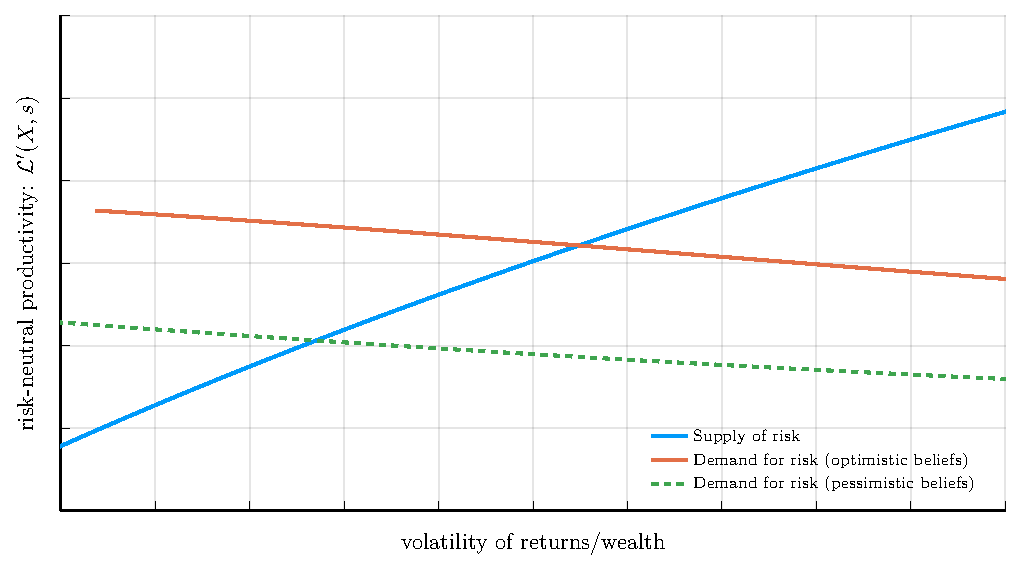
\includegraphics[width=0.99\textwidth]{figures/risk_equilibrium_inv.pdf}
            \caption{Market for risky assets}\label{fig: risk_eq}
        \end{minipage}
        \hfill
      \begin{minipage}[b]{0.5\textwidth}
        \centering
        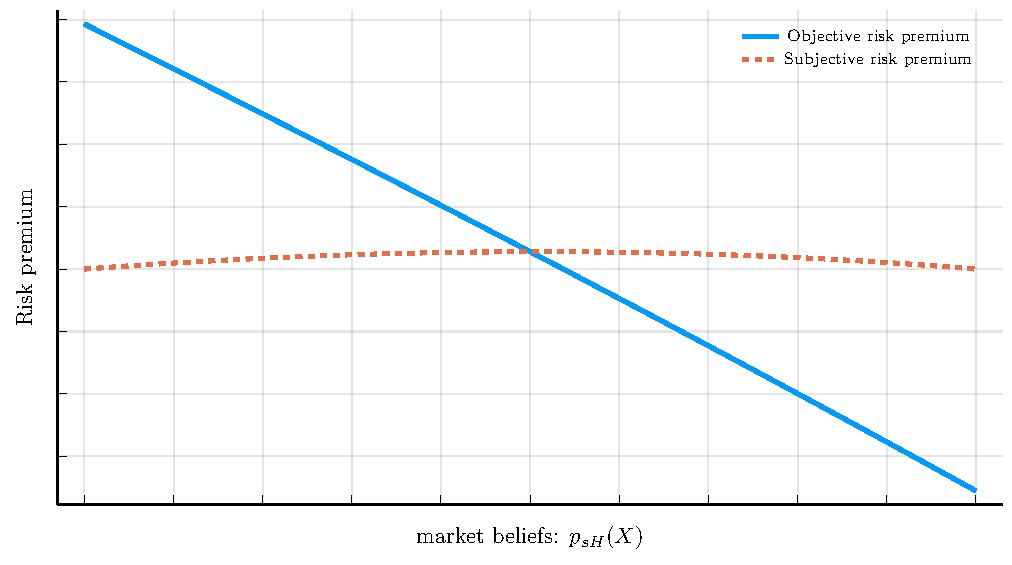
\includegraphics[width=0.99\textwidth]{figures/obj_subj_risk_premia.pdf}
            \caption{Beliefs and risk premia}\label{fig: obj_subj_risk_premia}
      \end{minipage}
      
      \end{minipage}    

    \end{figure}
Recall return volatility is proportional to dividend volatility. 
The supply of risk increases with $\mathcal{L}'(X,s)$ because dividend volatility increases with $\mathcal{L}'(X,s)$ due to the operating leverage channel. 
As firms hire more labor, profits are more exposed to productivity shocks, leading to higher volatility. 

The demand for risk is decreasing in $\mathcal{L}'(X,s)$. As shown in Proposition \ref{prop:asset_prices}, the risk premium is inversely related to $\mathcal{L}'(X,S)$, so investors are more willing to hold risky assets when the risk premium is high. 
The demand for risk is also a function of \textit{market beliefs}, a weighted average of investors' beliefs, $\overline{p}_{ss'}^m(X,s)$.
As market beliefs become more optimistic, investors are willing to hold more risky assets for a given risk premium.

Figure \ref{fig: risk_eq} illustrates how we can exploit this demand system representation to explain the effects of changes in market beliefs: 
When market beliefs become more pessimistic, there is a decline in the demand for risk, which leads to a decrease in the risk-neutral expected growth and, ultimately, a drop in employment. 

The following corollary formally demonstrates this by presenting the solution to the equilibrium risk-neutral expected growth as a function of market beliefs.
\begin{corollary}[Labor demand factor]\label{cor: Eprime} The risk-neutral expectation of productivity growth $\mathcal{L}'(X,s)$ is given by: 
\begin{equation}
    \mathcal{L}'(X,s)=\Gamma(X,s) - \sqrt{\Gamma(X,s)^{2}-\frac{1}{\alpha}  x_L x_H}.\nonumber
\end{equation}
where $\Gamma(X,s)$ is a function of market beliefs:
\[  
\Gamma(X,s)\equiv  \frac{\overline{p}^m_{sH}(X,s)}{2} \left(\frac{x_L}{\alpha} + x_H \right)+ \frac{\overline{p}^m_{sL}(X,s)}{2}\left(  x_L + \frac{x_H}{\alpha} \right).
\]
\end{corollary}
The key implication of Corollary~\ref{cor: Eprime} is that the risk-neutral expectation of productivity growth is \emph{entirely} determined by market beliefs. 
As a result, fluctuations in market beliefs translate directly into fluctuations in labor demand through firms' hiring decisions. 
Moreover, because market beliefs are a wealth-weighted average of individual beliefs, they depend on the distribution of wealth across investors. 
Changes in the wealth distribution therefore affect production through their impact on aggregate beliefs, providing a direct link between asset prices, labor demand, and the evolution of wealth inequality.


\q{RealEffects}{
\paragraph{The real effects of market beliefs.}

We have seen that, in our baseline economy, asset prices and labor demand are jointly
determined. The timing of hiring decisions is crucial for this result. To make this
point explicit, the next proposition shows that market beliefs have no real effects
when firms are allowed to adjust labor after productivity is realized.

\begin{proposition}[Real effects of market beliefs]
\label{prop:real_effects_beliefs}
Suppose firms choose hours after observing current productivity. Then hours, detrended
profits, and the return on the risky asset are independent of market beliefs:
\small
\begin{equation}
h(X,s)
=
\left(\frac{\alpha x_s}{\xi}\right)^{\frac{1}{1-\alpha}},
\qquad
\pi(X,s)
=
(1-\alpha)
\left(\frac{\alpha}{\xi}\right)^{\frac{\alpha}{1-\alpha}}
x_s^{\frac{1}{1-\alpha}},
\qquad
R_r(X,s,s')
=
\frac{x_s}{\beta}
\left(\frac{x_{s'}}{x_s}\right)^{\frac{1}{1-\alpha}}.
\end{equation}
\normalsize
Fluctuations in market beliefs affect the risk-free rate and the risk premium, but they
do not affect real variables or the expected return and volatility of the risky asset
under the objective measure.
\end{proposition}

Proposition~\ref{prop:real_effects_beliefs} establishes a form of
\emph{macro--finance separation} \citep{T00}: in the absence of a hiring friction,
belief-driven fluctuations in risk premia have asset-pricing implications but no real
effects on employment or output.

The timing assumption on hiring breaks this separation. When labor must be chosen in
advance, hiring is risky from the firm's perspective. An increase in optimism compresses
the risk premium, raises the value of risky assets, and---through the firm's optimality
condition---leads to higher employment. In this case, asset prices and labor demand are
simultaneously determined.

Absent fluctuations in market beliefs, employment would be constant in this economy,
consistent with the labor volatility puzzle documented by
\citet{shimer2010labor}. Section~\ref{sec:quantitative} explores the quantitative
implications of this mechanism by assessing how much labor volatility the model can
generate under empirically realistic fluctuations in beliefs.
}

\q{BeliefsAndRiskPremia}{
\paragraph{Beliefs and risk premia.}

Fluctuations in market beliefs generate movements in both risk premia
and labor demand. Why does optimism lead to changes in risk premia?

To answer this question, it is useful to distinguish between \emph{subjective} and
\emph{objective} risk premia. 
With a representative investor, the subjective risk premium is simply given by:
\begin{equation}
\mathbb E_{i,s}\!\left[R_r^e(X,s,s')\right]
\approx
\operatorname{Var}_{i,s}\!\left[R_r^e(X,s,s')\right].
\end{equation}
Thus, absent changes in perceived volatility, shifts in beliefs about average
productivity growth have little effect on the subjective risk premium in this case.

In contrast, the objective risk premium responds to differences in first moments. Using
the equilibrium expressions derived above, it can be written as
\begin{equation}
\mathbb E_s\!\left[R_r^e(X,s,s')\right]
=
\mathbb E_{i,s}\!\left[R_r^e(X,s,s')\right]
-
\frac{\mathbb E_{i,s}[x_{s'}]-\mathbb E_s[x_{s'}]}
{(1-\alpha)\mathcal L'(X,s)}.
\end{equation}
When investors become optimistic, they expect higher future dividends and bid up asset
prices. From the perspective of a rational investor, higher prices imply lower expected
returns going forward, compressing the objective risk premium.

Figure~\ref{fig: obj_subj_risk_premia} illustrates this mechanism. An increase in optimism,
captured by a rise in market beliefs $\overline p_{sH}^m(X,s)$, substantially reduces the
objective risk premium, while having a more muted effect on the subjective risk
premium. This pattern is consistent with empirical evidence documenting large movements
in expected returns with relatively stable subjective risk perceptions (see, e.g.,
\citealt{de_la_o_subjective_2021} and \citealt{nagel2023dynamics}).
}

\paragraph{The evolution of market beliefs.}
We have seen how market beliefs are determined by the wealth distribution. Next, we show how the wealth distribution evolves over time:
\begin{proposition}[Wealth dynamics]\label{prop: dynamics_beliefs} 
    The wealth share of investor $i\in \mathcal{I}$ evolves as:
        \begin{equation}
        \eta_i'(X,s,s') = \eta_i \frac{p^i_{ss'}}{\overline{p}^m_{ss'}(X,s)}.
    \end{equation}
    % \begin{enumerate}[(i)]
%     \item the wealth share of investor $i\in \mathcal{I}$ evolves as:
%     \begin{equation}
%     \eta_i'(X,s,s') = \eta_i \frac{p^i_{ss'}}{\overline{p}^m_{ss'}(X,s)},
% \end{equation}

%     \item market beliefs are:
%     \begin{equation}
%         \overline{p}^m_{s'H}(X',s') = \sum_{i=1}^I \eta_i \frac{p^i_{ss'}}{\overline{p}^m_{ss'}(X,s)} p_{s'H}^i.
%     \end{equation}
% \end{enumerate}
\end{proposition}
Proposition \ref{prop: dynamics_beliefs} shows that the wealth of household $i$ increases when she assigns a greater likelihood to the realized state than market beliefs. 

Next, we present a taxonomy of belief types. 
In particular, we discuss how different belief structures classified according to our taxonomy impact business cycles.

\subsection{Belief taxonomy and business-cycle properties}
\label{sec:belief_taxonomy.sec}

Although a large literature documents departures from full-information rational
expectations \citep{greenwood_expectations_2014, coibion2015information}, there is no
consensus on how precisely belief dynamics deviate from rational expectations.\footnote{Some
studies emphasize over-extrapolation \citep{bordalo2020overreaction, fuster2010natural},
as in models with diagnostic expectations \citep{bordalo2018diagnostic} or fading memory
\citep{nagel2022asset}. Others emphasize under-reaction, such as sticky information
\citep{mankiw2010imperfect}, cognitive discounting \citep{gabaix2019behavioral}, and
level-$k$ thinking \citep{farhi2019monetary}.} This section classifies belief structures
and shows how each maps into distinct business-cycle implications. We organize the
analysis around the following taxonomy.

\begin{definition}[Taxonomy of beliefs]
\label{def: belief_taxonomy}
\q{Taxonomy}{
Household $i$ is \emph{optimistic} (\emph{pessimistic}) relative to a benchmark belief
$o$ in state $s$ if $p_{sH}^i > p_{sH}^o$ ($p_{sH}^i < p_{sH}^o$). We further distinguish
two classes of belief dynamics:
\begin{enumerate}[(i)]
\item \textbf{Rank-preserving beliefs}: household $i$ is optimistic or pessimistic
relative to $o$ in all states.
\item \textbf{Rank-alternating beliefs}: household $i$ is optimistic relative to $o$ in
one state but pessimistic in the other.
\end{enumerate}
}
\end{definition}

The benchmark belief $o$ can represent either rational expectations or the beliefs of
another household. This taxonomy allows us to characterize how different belief
structures affect both the amplitude and the phase of business-cycle fluctuations.

\paragraph{Homogeneous beliefs.}

With homogeneous beliefs, the risk-neutral expectation of productivity growth,
$\mathcal L'(X,s)$, depends only on current productivity. 
Therefore, the models lacks an internal propagation mechanism, as there is no variation in hours in the absence of changes in productivity growth. 
Moreover, if
investors believe productivity growth is i.i.d., so that $p_{LH}^i=p_{HH}^i$, then
$\mathcal L'(X,s)$ and, consequently, hours are constant over time.

Away from i.i.d.\ beliefs, homogeneous beliefs can either amplify or dampen fluctuations. Figure~\ref{fig: hom_beliefs} illustrates
this point by simulating four periods of recession within a twenty-period interval for
five belief specifications: rational expectations
($p_{ss'}^i=p_{ss'}$ for all $s,s'$); two rank-preserving cases---always optimistic
($p_{sH}^i>p_{sH}$ for all $s$) and always pessimistic ($p_{sH}^i<p_{sH}$ for all $s$);
and two rank-alternating cases---\emph{extrapolative} beliefs, defined as optimistic in
booms and pessimistic in recessions, and \emph{contrarian} beliefs, defined as
pessimistic in booms and optimistic in recessions.

Optimistic rank-preserving beliefs amplify expansions but dampen recessions relative to
rational expectations, while pessimistic rank-preserving beliefs have the opposite
effect. Thus, rank-preserving beliefs generate state-dependent amplification.

Rank-alternating beliefs operate differently. Under extrapolative beliefs, optimism in
booms and pessimism in recessions magnify the amplitude of the cycle. By contrast, contrarian beliefs dampen fluctuations by reducing
labor demand in booms and supporting it in recessions. Overall, extrapolative beliefs are
the belief structure that most strongly amplifies business-cycle fluctuations relative
to rational expectations.

\begin{figure}[t!]
    \centering
            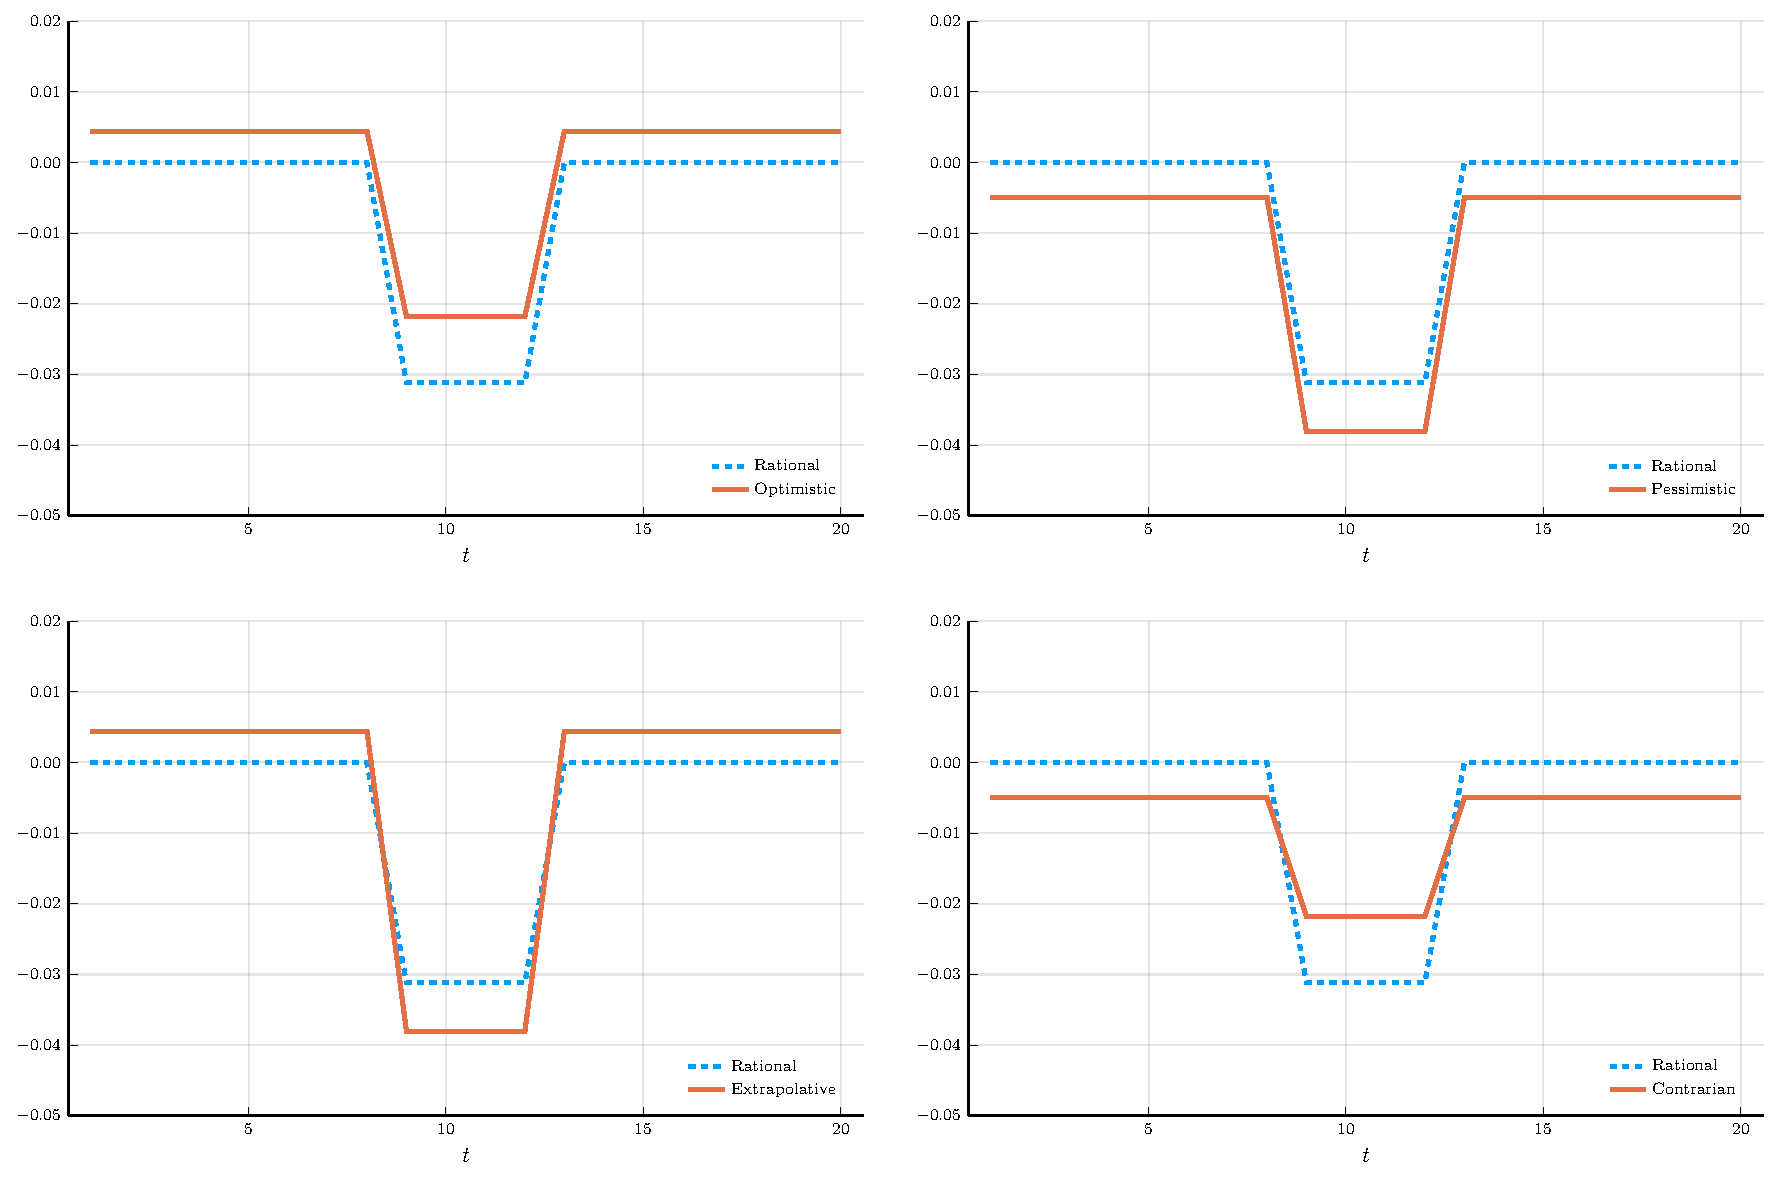
\includegraphics[width=0.90
            \textwidth]{figures/simul_hom_beliefs.pdf}
    \caption{Homogeneous beliefs}
    \caption*{  \scriptsize 
    Note: examples of cycles (four periods of bad shocks with sixteen periods of expansions) for log labor hours with homogeneous beliefs: rational, always optimistic (top-left panel), always pessimistic (top-right panel), extrapolative (bottom-left panel), and contrarian (bottom-right panel) beliefs. \par} 
    \vspace{0.0cm}
    \label{fig: hom_beliefs}
\end{figure}

\paragraph{Heterogeneous beliefs.}

Next, we investigate the role of belief heterogeneity. 
It is well known that RBC models typically have very weak internal propagation mechanisms \citep{cogley1995output}.
With heterogeneous beliefs and labor chosen one period in advance, the model features an important internal propagation mechanism: the wealth distribution, and market beliefs, evolve over time even without changes in the productivity state.
% The model now features an internal propagation mechanism, as the wealth distribution, and market beliefs, evolve over time even without changes in the productivity state.
From Proposition~\ref{prop: dynamics_beliefs}, optimists accumulate wealth during booms and lose
wealth during downturns. This observation is key to understanding the model dynamics.

\begin{corollary}\label{cor:het_dynamics}
If beliefs are heterogeneous, then:
\begin{itemize}
\item Conditional on remaining in the same state, the risk-neutral expectation of
productivity growth $\mathcal L$ increases (decreases) over time in the high-growth
(low-growth) state.
\item Consider an initial state $(X,H)$ and a transition from $H$ to $L$ at some future
date. Then:
\begin{itemize}
\item If beliefs are \emph{rank-preserving}, a longer boom leads to a smaller subsequent
decline in output.
\item If beliefs are \emph{rank-alternating}, a longer boom leads to a larger subsequent
decline in output.
\end{itemize}
\end{itemize}
\end{corollary}

% \begin{proof}
% See Appendix~\ref{app: proof_cor_het_dynamics}.
% \end{proof}

With belief heterogeneity, the economy evolves even in the absence of changes in
productivity growth. 
During booms, optimistic investors accumulate wealth, causing market beliefs to become
more optimistic relative to rational expectations and increasing labor demand. The
opposite occurs during prolonged low-growth phases, when pessimistic investors gain
wealth and market beliefs tilt toward pessimism.

\begin{figure}[t!]
    \centering
            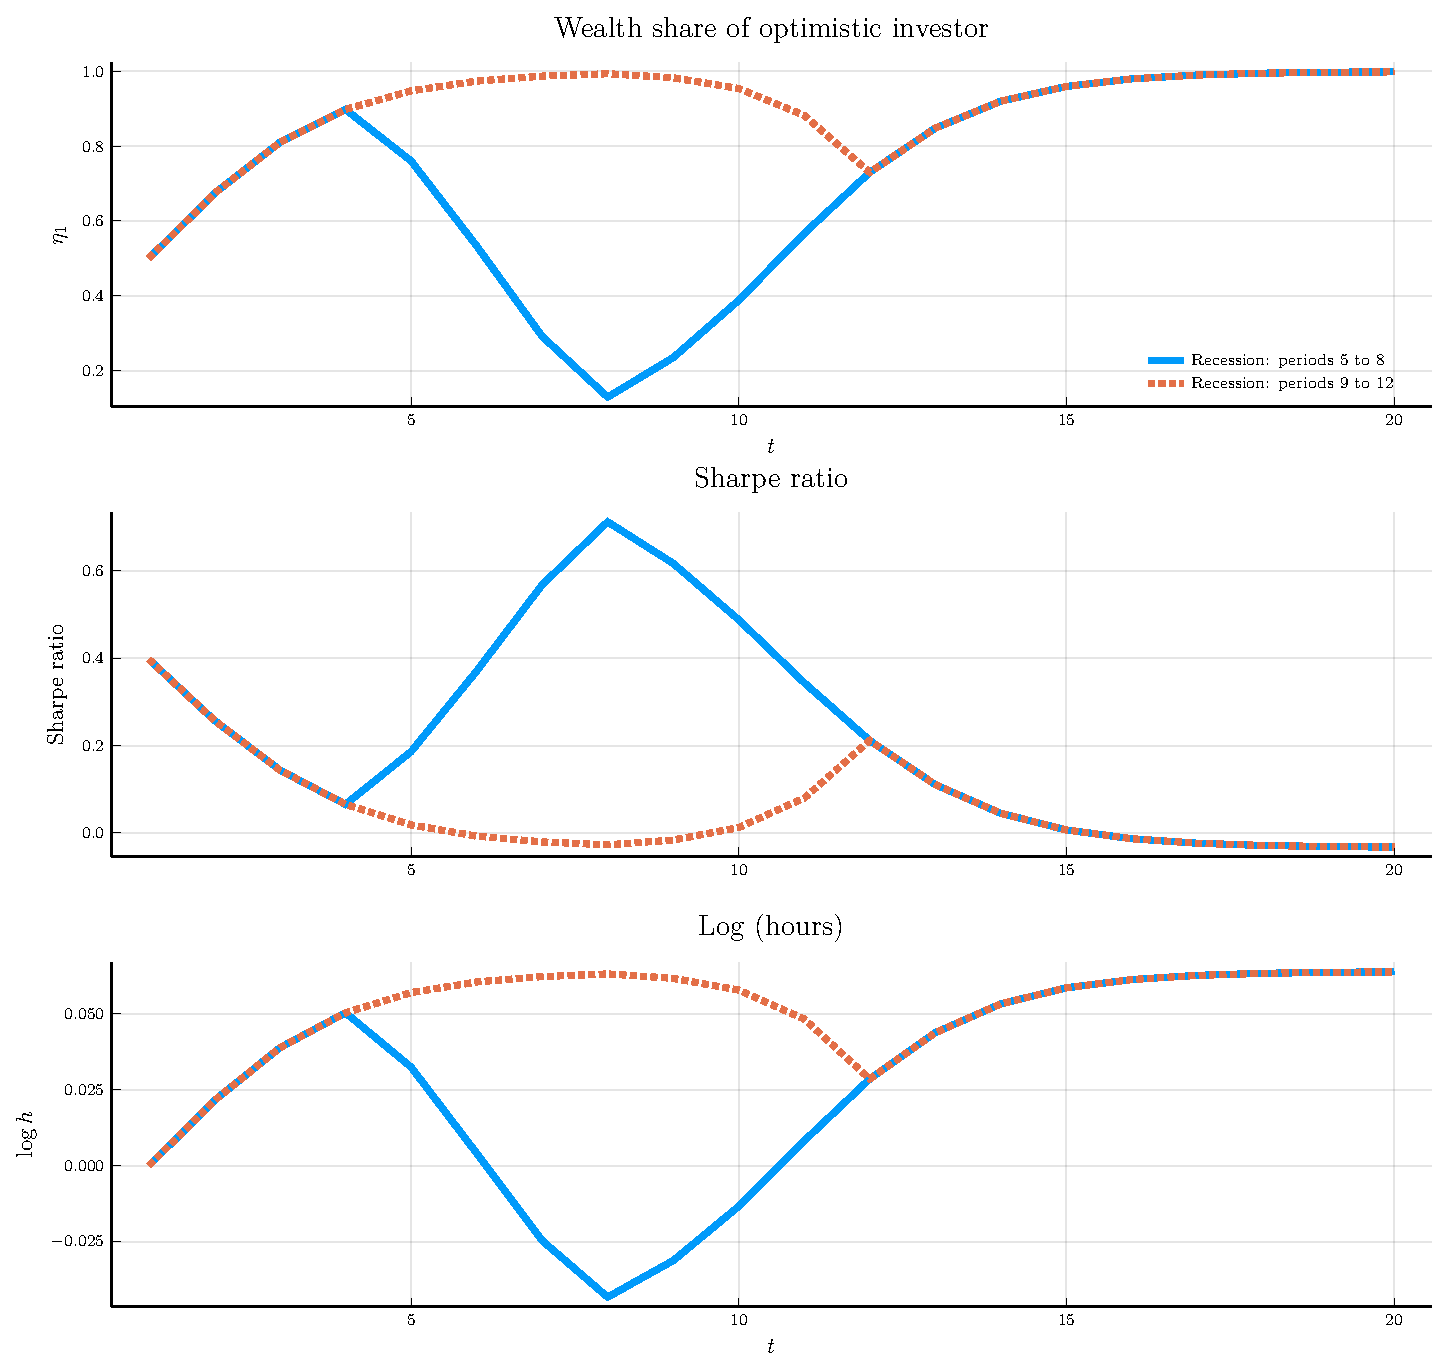
\includegraphics[width=0.75
            \textwidth]{figures/simul_het_beliefs1.pdf}
    \caption{Heterogeneous beliefs: optimistic vs pessimistic}
    \caption*{  \scriptsize 
    Note: examples of cycles (four periods of bad shocks with sixteen periods of expansions) with heterogeneous beliefs: $I=2$ investors, always optimistic and always pessimistic. The top panel shows the wealth share of the optimistic investor, the middle panel shows the Sharpe ratio (under objective beliefs), and the bottom panel shows log labor hours. \par} 
    \vspace{0.0cm}
    \label{fig: het_beliefs1}
\end{figure}

Figure~\ref{fig: het_beliefs1} illustrates this mechanism for the case of rank-preserving
beliefs. The figure shows simulations with two investors, one optimistic and one
pessimistic in all states. The top panel displays the optimist's wealth share, the middle
panel the objective Sharpe ratio, and the bottom panel log labor hours. As the economy
remains longer in the high-growth state, the optimist accumulates more wealth. 
This reduces the Sharpe ratio (i.e., the price of risk), and increases labor demand.
When the
economy eventually transitions to the low-growth state, the greater wealth share of
optimistic investors mitigates the increase in risk premia and attenuates the decline in
hours.

Figure~\ref{fig: het_beliefs2} presents the corresponding case of rank-alternating beliefs,
with one rational and one extrapolative investor. During booms, extrapolative investors
accumulate wealth, but they become pessimistic when the economy transitions to the
low-growth state. As a result, market beliefs turn sharply pessimistic during downturns,
leading to a larger increase in risk premia and a more pronounced contraction in labor
demand.
Hence, the longer the boom, the greater the bust.


\begin{figure}[t!]
    \centering
            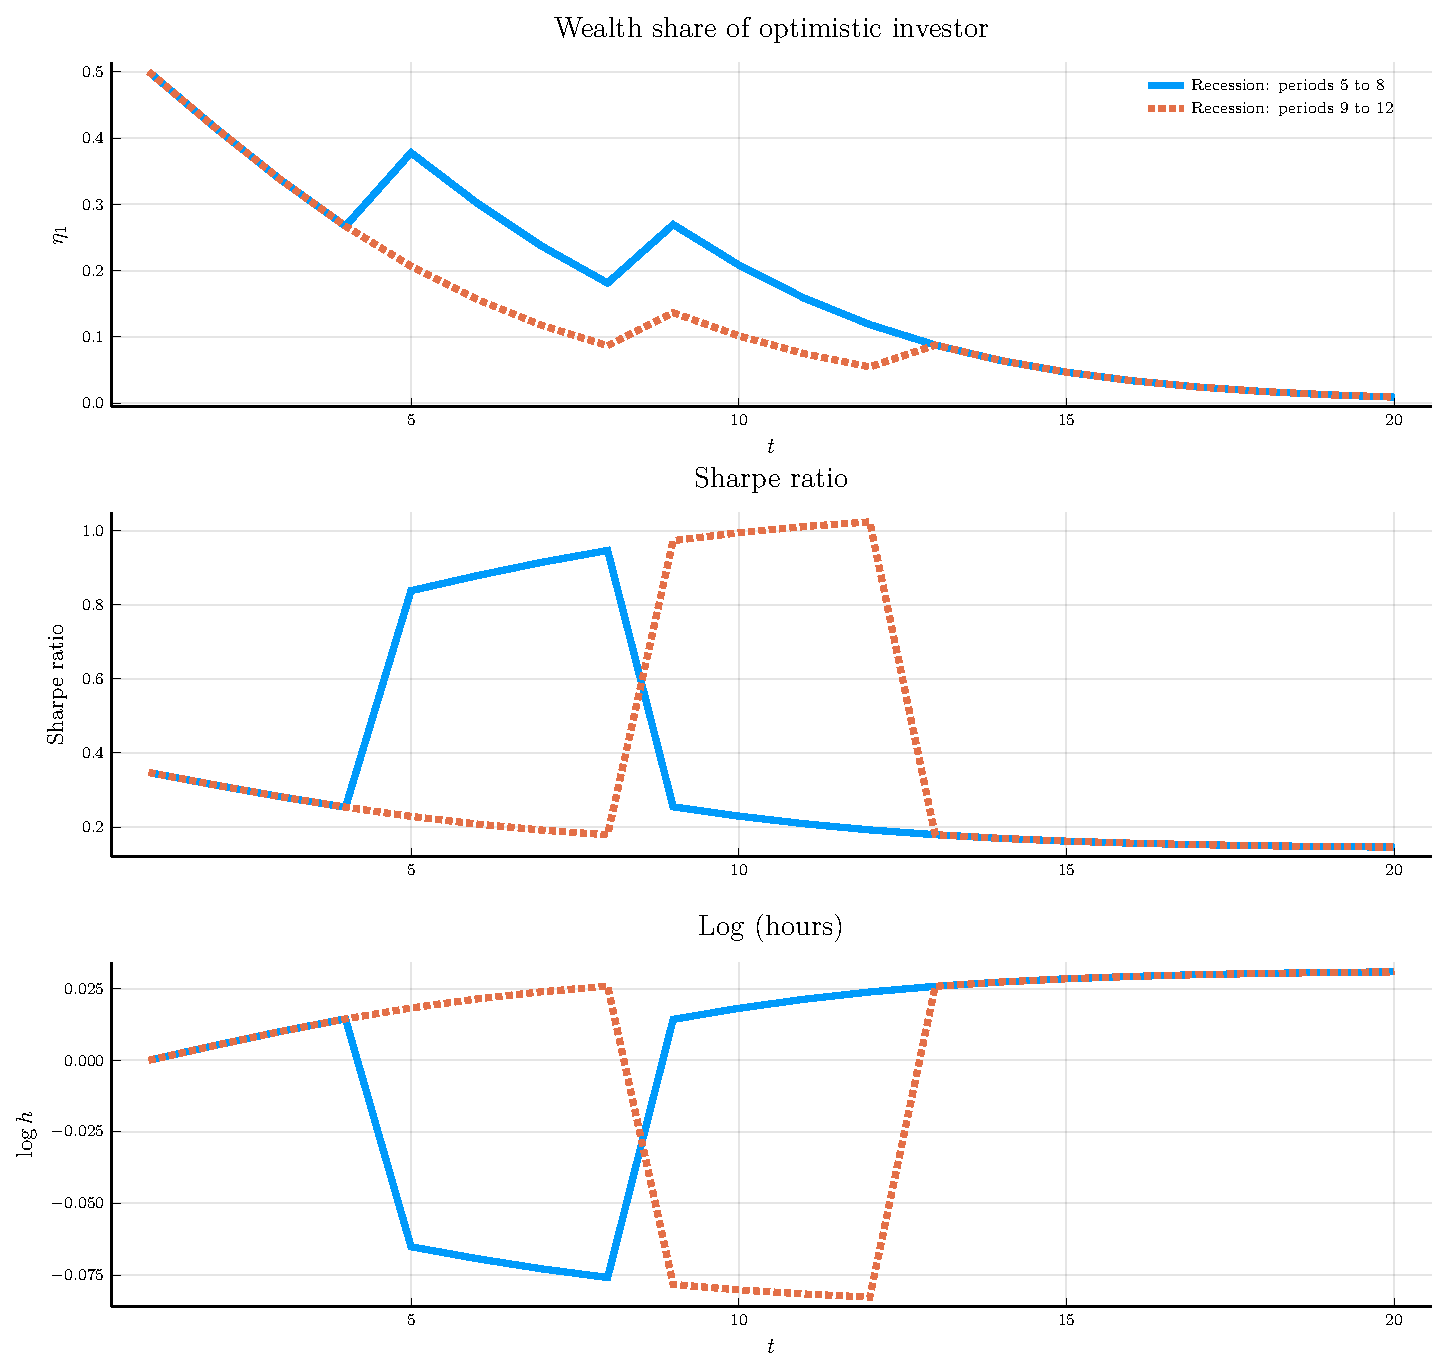
\includegraphics[width=0.75
            \textwidth]{figures/simul_het_beliefs2.pdf}
    \caption{Heterogeneous beliefs: rational vs extrapolative}
    \caption*{  \scriptsize 
    Note: examples of cycles (four periods of bad shocks with sixteen periods of expansions) with heterogeneous beliefs: $I=2$ investors, rational and extrapolative. The top panel shows the wealth share of the optimistic investor, the middle panel shows the Sharpe ratio (under objective beliefs), and the bottom panel shows log labor hours. \par} 
    \vspace{0.0cm}
    \label{fig: het_beliefs2}
\end{figure}

\q{RoleRiskAversion}{
\paragraph{The role of risk aversion.}

The results above rely on two key features of the wealth dynamics. First, the wealth
share of optimistic investors increases during booms and decreases during recessions.
Second, as implied by Proposition~\ref{prop: dynamics_beliefs}, the future wealth share of
any investor is increasing in her current wealth share:
\begin{equation}
\frac{\partial \eta_i'(X,s,s')}{\partial \eta_i}
=
\frac{p^i_{ss'}}{\overline p^m_{ss'}(X,s)}
-\eta_i\,\frac{p^i_{ss'}\bigl(p^i_{ss'}-p^I_{ss'}\bigr)}{\left(\overline p^m_{ss'}(X,s)\right)^2}
=
\frac{p^i_{ss'}}{\left(\overline p^m_{ss'}(X,s)\right)^2}
\left(\sum_{j\neq i}\eta_j p^j_{ss'}+\eta_i p^I_{ss'}\right)
\ge
0,\nonumber
\end{equation}
and it is strictly positive if, e.g., $p^j_{ss'}>0$ for all $j$.

This property contrasts with models featuring risk-neutral investors, in which optimistic
agents are driven to concentrate their wealth in the good state and are wiped
out in the bad state \citep{G10}. With risk-averse investors, by contrast,
agents choose to allocate wealth across both states of the world. As a result, optimistic
investors retain wealth in downturns, allowing the belief-driven amplification mechanism
to operate.

The strength of this mechanism depends on the degree of risk aversion. When optimistic
investors are close to risk-neutral, additional wealth accumulated during a boom is
largely tilted toward the good state, attenuating the amplification of fluctuations in
bad times. Higher risk aversion induces investors to distribute wealth more evenly across
states, increasing the influence of optimistic investors during downturns and thereby
strengthening the amplification of adverse shocks.
}

\q{FrothyMarkets}{\paragraph{Frothy markets and risk build-ups.}

An implication of Corollary~\ref{cor:het_dynamics} is that the risk premium declines
with the length of economic expansions. To the extent that risk premia are reflected
in credit spreads, the model is consistent with the discussion in
\citet{lopez2017credit} and \citet{krishnamurthy2017credit} that economic booms
are characterized by ``frothy'' market conditions driven by credit-market sentiment.

Importantly, the model delivers a joint prediction: as optimism builds during
prolonged expansions, objective risk premia decline while dividend volatility rises.
The compression in spreads reflects the greater risk-bearing capacity of optimistic
investors. At the same time, lower risk premia raise labor demand, increase the labor
share, and amplify operating leverage. Because labor is chosen in advance,
profits, and therefore dividends, become more sensitive to productivity shocks.
This combination implies an endogenous \emph{risk build-up} during booms:
fragility increases precisely when spreads are low.

As emphasized by \citet{krishnamurthy2020dissecting}, generating simultaneously
low spreads and rising risk exposure is challenging in standard macro-finance models,
such as \citet{he2013intermediary} and \citet{brunnermeier2014macroeconomic}.
In contrast, heterogeneous extrapolative beliefs naturally generate this pattern
in our framework.

Each link in this mechanism is supported by existing evidence. First, survey-based
measures of optimism are associated with lower expected returns, consistent with
compressed risk premia (e.g., \citealt{de_la_o_subjective_2021}). Second, measures of
labor demand and labor share predict lower future stock returns
(\citealt{santos2006labor, belo2023drives}), consistent with the link between labor demand
and risk premia. Third, higher labor share is associated with stronger operating leverage
and greater sensitivity of profits to shocks (\citealt{donangelo2019cross}). Taken together,
these findings support the interpretation that periods of elevated optimism are
characterized by compressed spreads and increased fragility.}
% \paragraph{Frothy markets and risk build-ups.} An implication of Corollary \ref{cor:het_dynamics} is that the risk premium declines with the length of economic expansions. 
% To the extent that risk premia drive credit spreads, the model is consistent with the discussions in \citet{lopez2017credit} and \citet{krishnamurthy2017credit} that argue that economic booms are characterized by "froth" market conditions driven by credit-market \textit{sentiments}. 
% Our framework shows that with belief extrapolation, an increase in optimism leads to a reduction in risk premia and an increase in volatility, as shown in Figure \ref{fig: risk_eq}. Under this interpretation, there is endogenous \textit{risk build-up} during booms. 
% As argued by \citet{krishnamurthy2020dissecting}, the combination of risk build-up and low spreads is challenging to generate for standard macro-finance models, such as \citet{he2013intermediary} and \citet{brunnermeier2014macroeconomic}. This observation suggests that heterogeneous extrapolative beliefs explain credit and asset-market dynamics during boom-bust cycles.

% \q{ExogenousBuildUp}{It is worth clarifying that risk-build-up requires heterogeneity only when beliefs about the state are themselves Markovian. If beliefs are history-dependent, for example, if agents become more optimistic as boom states persist but more pessimistic once the economy switches states as boom states persist, the economy can also feature risk build-up. 
%         This risk build-up would not respond to the model's internal propagation through leverage, risk-exposure, and wealth accumulation, though.}

% \paragraph{Discussion: Pareto and Belief-Neutral Welfare.} 

% \q{ParetoEfficiency}{The environment's inherent risk build-up leads to subtle normative implications. 
% It is well known that, under complete markets, the equilibrium is Pareto efficient from a subjective standpoint. 
% The First Welfare Theorem does not distinguish whether trade is driven by differences in preferences over goods or by differences in beliefs across future states--- treating both as equally valid sources of heterogeneity.} 

% \q{NeutralWelfare}{Classic Pareto efficiency is not the only sensible welfare criterion. \citet{BrunnermeierSimsekXiong2014} considers a paternalistic criterion, albeit one that does not presume superior knowledge by the planner. Instead, this belief-neutral criterion only requires the allocation to be efficient for all possible (convex combinations of) the agents' beliefs. Our environment is generically inefficient under this belief-neutral criterion: the simplest way to see this is to assume all agents believe TFP growth is iid but differ in the weights they assign states. In such a case, under all possible belief combinations, TFP growth is iid. Hence, labor fluctuations are inefficient under this criterion. This criterion can be used to justify leaning against the wind policies even though the economy is efficient in a standard sense.}


\q{RiskAversionDiscussion}{\paragraph{Discussion: belief heterogeneity vs. risk aversion.}
As discussed above, rank-alternating beliefs amplify inherent economic fluctuations.
The key distinction is that heterogeneity in beliefs can induce changes in the 
\emph{ranking} of investors' effective risk-taking across states.
In models with heterogeneous risk aversion, differences in risk tolerance can generate
portfolio dispersion and time variation in expected returns. However, the ranking of
agents in terms of risk-taking is fixed: the more risk-tolerant agent always holds
more risky assets in every state of the world. This property is analogous to the
case of rank-preserving beliefs shown in Figure~\ref{fig: het_beliefs1}.
In contrast, under rank-alternating beliefs, the identity of the relatively
risk-taking investor depends on the state. An agent who takes more risk in booms
may take less risk in busts. There is no counterpart to this mechanism in models
with heterogeneous risk aversion alone.
}

\subsection{Belief taxonomy and trading volume}\label{sec: trading_volume}
\q{TradingVolumeTheory}{

Our belief taxonomy also has sharp implications for trading dynamics. As is standard in
models with belief heterogeneity, trading volume is closely related to the degree of
disagreement among investors. We show that not only the level but also the \emph{type} of
disagreement---as classified in Definition~\ref{def: belief_taxonomy}---plays a central role
in shaping the dynamics of trading volume over the business cycle.

\subsubsection{Analytical characterization of turnover}
We adopt \emph{share turnover} as our measure of trading volume, following
\citet{lo2000trading}, defined as
\begin{equation}
    \tau_t \equiv \frac{1}{2}\sum_{i=1}^I \mu_i \big|S_{i,t}-S_{i,t-1}\big|
    = \frac{1}{2}\sum_{i=1}^I \big|\omega_{i,t}\eta_{i,t}-\omega_{i,t-1}\eta_{i,t-1}\big|,
    \nonumber
\end{equation}
where we divide by two to avoid double counting trades, and the second equality uses
$\mu_i S_{i,t}=\omega_{i,t}\eta_{i,t}$.

In the absence of belief heterogeneity, $\omega_{i,t}=1$ and $\eta_{i,t}=\eta_{i,t-1}$, so
$\tau_t=0$. With heterogeneous beliefs, turnover depends on the extent of belief dispersion.
To characterize this dependence analytically, we consider a small deviation from a
homogeneous-beliefs benchmark. Specifically, assume
\begin{equation}
    p_{ss'}^i = p_{ss'}^* + \delta_{ss'}^i \epsilon,\qquad \delta_{sH}^i+\delta_{sL}^i=0,
    \nonumber
\end{equation}
where $p_{ss'}^*$ denotes the common belief in the benchmark and $\epsilon$ controls the
degree of dispersion. For simplicity, we take the benchmark belief to be symmetric and
i.i.d., $p_{ss'}^*=\tfrac{1}{2}$. Appendix~\ref{app: proof_lemma_trading} discusses the general case.

In this neighborhood, the portfolio share and next-period wealth share of investor $i$ admit the expansions\small
\begin{equation}
    \omega_i(X,s) = 1 + \kappa_\omega\!\left[p_{sH}^i-\overline{p}^{\,m}_{sH}(X,s)\right]+\mathcal{O}(\epsilon^2),
    \qquad
    \eta_i'(X,s,s') = \eta_i + \eta_i\frac{p_{ss'}^i-\overline{p}^{\,m}_{ss'}(X,s)}{p_{ss'}^*}
    + \mathcal{O}(\epsilon^2),
    \nonumber
\end{equation}\normalsize
where $\kappa_\omega>0$ and $\overline{p}^{\,m}_{ss'}(X,s)\equiv\sum_{j=1}^I\eta_j p_{ss'}^j$
denotes market beliefs. These expressions highlight how differences in beliefs drive portfolios and wealth dynamics.

To understand the determinants of trading volume, it is useful to decompose individual
trading into two distinct components. The following lemma expresses an investor's net purchases as the sum of a rebalancing motive
and a relative belief-updating motive.

\begin{lemma}\label{lem:trading}
Investor $i$'s net purchases of shares are given by
\begin{equation}\label{eq:trading}
    \mu_i \Delta S_i(X,s,s';\epsilon)
    =
    \underbrace{\Delta \eta_i(X,s,s')}_{\text{rebalancing effect}}
    +
    \underbrace{\Delta \omega_i(X,s,s')\,\eta_i}_{\text{change-in-beliefs effect}}
    + \mathcal{O}(\epsilon^2),
\end{equation}
where\small
\begin{align}
    \Delta \eta_i(X,s,s') &\equiv \eta_i \frac{p_{ss'}^i-\overline{p}^{\,m}_{ss'}(X,s)}{p_{ss'}^*},
    \qquad
    \Delta \omega_i(X,s,s') \equiv \kappa_\omega\!\left[
        \big(p_{s'H}^i-\overline{p}^{\,m}_{s'H}(X,s)\big)
        -\big(p_{sH}^i-\overline{p}^{\,m}_{sH}(X,s)\big)
    \right].
    \nonumber
\end{align}\normalsize
\end{lemma}

Lemma~\ref{lem:trading} shows that individual trading behavior is governed by two distinct forces.
The \emph{rebalancing effect} captures trades required to maintain a constant portfolio share
following changes in relative wealth. This effect occurs because when an optimistic investor gains wealth
after a favorable shock, she must purchase additional shares to keep her portfolio composition unchanged.
The \emph{change-in-beliefs effect} reflects active portfolio reallocation driven by revisions in
relative beliefs across states: if an investor becomes more optimistic in state $s'$ than in state $s$,
she increases her exposure to the risky asset upon the transition.

Whether these two effects reinforce or offset each other depends on how beliefs evolve across states.
This interaction is the key mechanism behind the state-dependent relationship between belief dispersion
and trading volume.


\paratitle{Turnover and belief taxonomy.} As in Section~\ref{sec:environment.sec}, we can express beliefs in terms of a persistence parameter, $\rho_i$, and a bias term, $\Delta_i$:
\begin{equation}\label{eq: beliefs_persistence_bias}
    p_{HH}^i = \frac{1+\rho_i}{2} + \Delta_i, \qquad \qquad p_{LH}^i = \frac{1-\rho_i}{2} + \Delta_i,\nonumber
\end{equation}
which implies that the conditional expectation of productivity growth is given by:
\begin{equation}\label{eq: conditional_expectation}
    \mathbb{E}_{i,t}[x_{t+1}] = \overline{x}_i + \rho_i (x_t - \overline{x}_i),
\end{equation}
where $\overline{x}_i$ is the subjective unconditional mean of $x_t$.

Consider first the case of rank-preserving beliefs, $\rho_i = \rho$, where investors differ on the level of optimism, $\Delta_i$. 
% In this case, beliefs are constant, $p_{HH'}^i = p_{LL'}^i = \frac{1+\rho}{2}$, and turnover is given by:
In this case, the change-in-beliefs effect vanishes and turnover is driven
solely by the rebalancing effect:
\begin{equation}
    \tau(X,s,s';\epsilon)
    =
    \sum_{i=1}^I \eta_i
    \big|p_{ss'}^i-\overline{p}^{\,m}_{ss'}(X,s)\big|
    +\mathcal{O}(\epsilon^2).
    \nonumber
\end{equation}
In this case, turnover is proportional to the average absolute deviation of beliefs, a natural
measure of belief dispersion, so trading volume increases with disagreement.

Consider next the case of rank-alternating beliefs, $\Delta_i = \Delta$, where investors differ on the persistence parameter, $\rho_i$. 
In this case, the change-in-beliefs effect emerges when the economy switches states, $s\neq s'$, and it may either
amplify or dampen the rebalancing effect. 
For instance, suppose the
economy switches from $H$ to $L$. Investors who were relatively
optimistic in the boom lose wealth on impact and, at the same time, become relatively pessimistic in
the downturn. Both forces push toward selling, so turnover rises sharply. By contrast, when the
economy switches from $L$ to $H$, the same investors become relatively optimistic and wish to raise
their risky share, while rebalancing incentives work in the opposite direction because their wealth share decreases. Turnover is therefore more sensitive to disagreement in recessions than in expansions.

% To formalize this asymmetry, consider a rank-alternating specification in which investors agree on the
% unconditional mean of productivity growth, $\overline{x}$, but disagree about persistence, $\theta_i$:
% \begin{equation}\label{eq: persistence}
%     \mathbb{E}_{i,t}[x_{t+1}] - \overline{x} = \theta_i\,(x_t-\overline{x}),
% \end{equation}
% where $\theta_i$ is a function of $p_{ss'}^i$. 
The next proposition formalizes this intuition and delivers the central result of this
section: trading volume is increasing in belief dispersion, and this relationship is asymmetric over the
business cycle under rank-alternating beliefs.

\begin{proposition}\label{prop:turnover}
Suppose investors' beliefs are rank-alternating, that is, they are given by \eqref{eq: beliefs_persistence_bias} with $\Delta_i = \Delta$. Turnover as the economy switches from $s$ to $s'$ is given by
\begin{equation}
    \tau(X,s,s';\epsilon)
    =
    \frac{\zeta(s,s')}{2}\sum_{i=1}^I \eta_i \big|\rho_i-\rho(X)\big|
    +\mathcal{O}(\epsilon^2),
    \nonumber
\end{equation}
where $\rho(X) \equiv \sum_{i=1}^I \eta_i \rho_i$, and
\begin{equation*}
    \zeta(s,s') \equiv
    \left\{
    \begin{array}{ll}
        \kappa_\omega+1, & \text{if } s=H \text{ and } s'=L,\\
        \big|\kappa_\omega-1\big|, & \text{if } s=L \text{ and } s'=H,\\
        1, & \text{if } s=s'.
    \end{array}
    \right.
\end{equation*}
\end{proposition}

The key message from Proposition~\ref{prop:turnover} is that turnover increases with belief dispersion and,
furthermore, that this sensitivity is stronger in downturns. The assumption of rank-alternating beliefs is essential for generating this asymmetry. With rank-preserving beliefs---investors are relatively
optimistic or pessimistic by the same amount in both states---the change-in-beliefs effect is absent, and turnover is driven primarily by rebalancing. Hence, disagreement does not generate a disproportionately strong response of trading volume in bad times. Thus, rank-alternating beliefs are key to inducing state-dependent dynamics of stock market turnover.
}


\subsubsection{Empirical evidence}

\begin{figure}[t!]
    \caption{Disagreement Index and Stock Market Turnover}
    \centering
    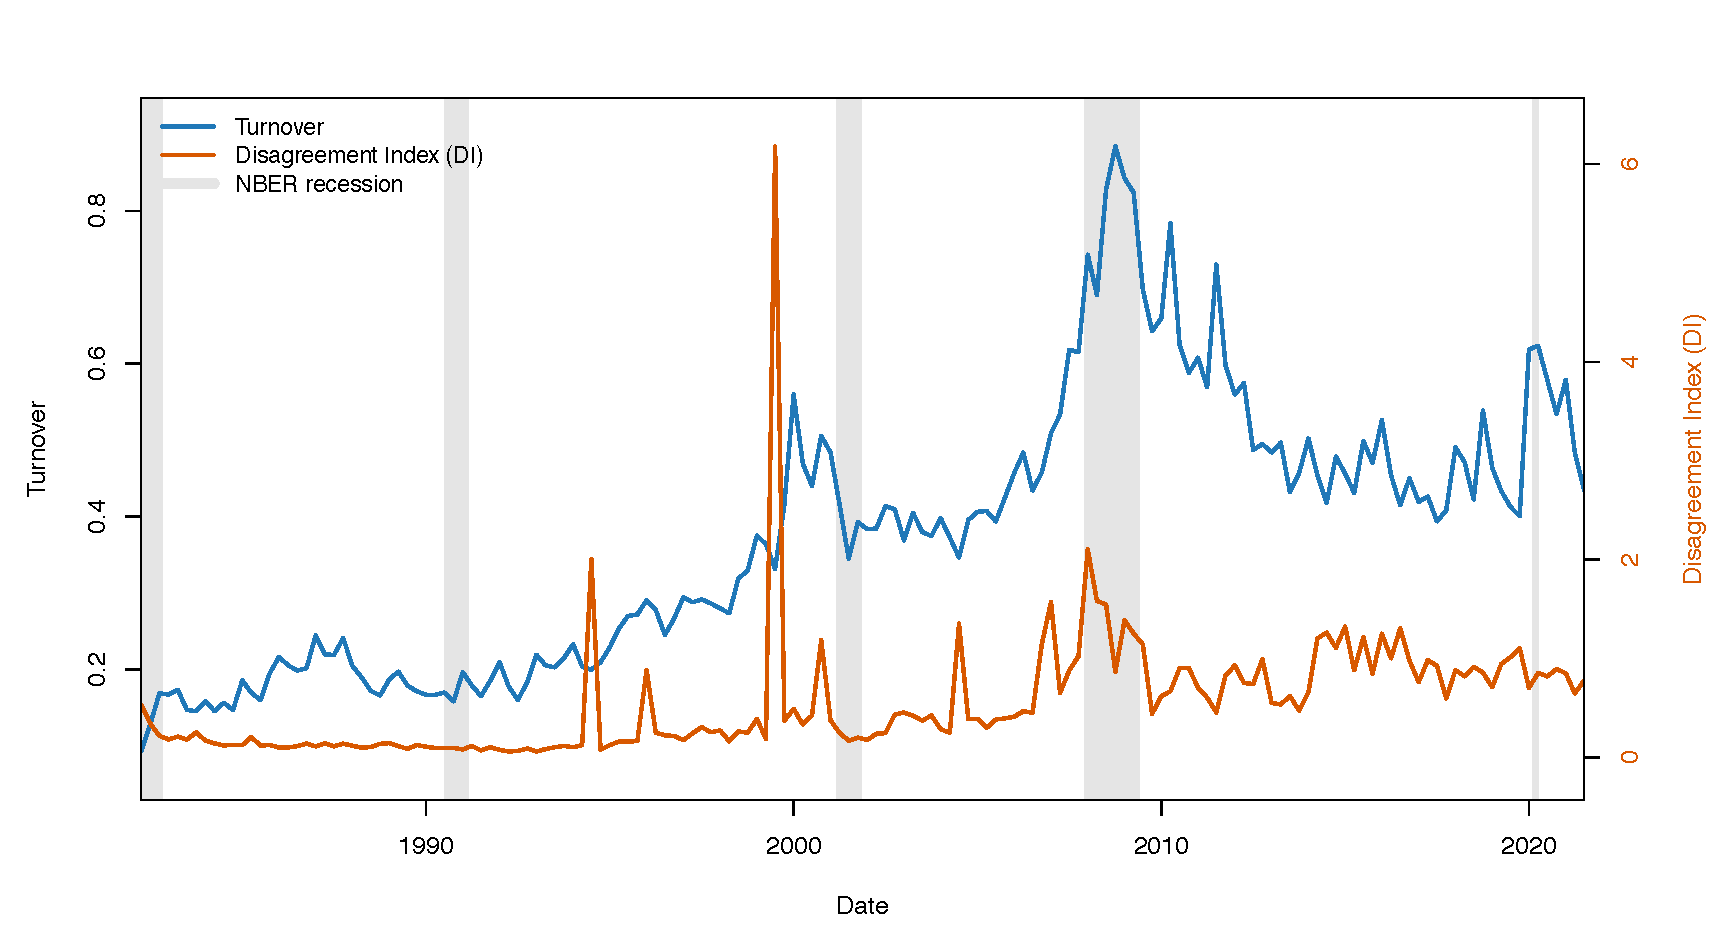
\includegraphics[width=0.9\textwidth]{figures/turnover_vs_disagreement_index.pdf}
    \label{fig: DI_turnover_time_series}
\end{figure}

\q{EmpiricalEvidenceI}{We now test the model's prediction that trading volume increases with belief
dispersion and that this sensitivity is stronger during downturns.

\paragraph{Measuring disagreement and turnover.}

The model links trading dynamics to disagreement about aggregate shocks.
To construct an empirical analogue, we combine analyst forecasts from I/B/E/S
with stock market turnover from CRSP.

Let $\mathbb{E}_{j,t}[\Delta e_{i,t+1}]$ denote analyst $j$'s forecast of
firm $i$'s earnings growth at time $t$, and let $\Delta e_t$
denote realized aggregate earnings growth.
To isolate the analyst-specific component reflecting beliefs about aggregate dynamics,
we estimate
\begin{equation}
    \mathbb{E}_{j,t}[\Delta e_{i,t+1}]
    =
    \alpha_{i,t}
    +
    \beta_{0,j}
    +
    \beta_{1,j} \Delta e_t
    +
    u_{j,i,t},
\end{equation}
where $\alpha_{i,t}$ is a firm--time fixed effect,
$\beta_{0,j}$ is an analyst-specific intercept,
$\beta_{1,j}$ captures the analyst's sensitivity to aggregate earnings growth,
and $u_{j,i,t}$ is an error term.

The firm--time fixed effect absorbs firm-level information common to all analysts.
The remaining analyst-specific terms therefore capture systematic differences in beliefs
about aggregate earnings dynamics.
We interpret the implied aggregate expectation of analyst $j$ as
\[
\mathbb{E}_{j,t}[\Delta e_{t+1}]
=
\beta_{0,j} + \beta_{1,j} \Delta e_t,
\]
which mirrors the model's specification of expected productivity growth
in Equation~\eqref{eq: conditional_expectation}.

We then construct a time-varying \emph{disagreement index} as the cross-sectional
dispersion of these implied aggregate expectations:
\begin{equation}
    DI_t
    =
    \overline{\sigma}_t\!\left[\beta_{0,j} + \beta_{1,j} \Delta e_t \right],
\end{equation}
where $\overline{\sigma}_t[\cdot]$ denotes the cross-sectional standard deviation at time $t$. 

While analyst-specific coefficients are constant over time, time changes in disagreement occur through $\Delta e_t$. This reflects the model's mechanism that dispersion in persistence beliefs interacts
with the current state of the economy.

To measure trading activity, we follow \citet{lo2000trading} and compute
value-weighted stock market turnover from CRSP.\footnote{
Details on construction are provided in Appendix~\ref{app:data_turnover}.}

Figure~\ref{fig: DI_turnover_time_series}
plots the time series of the disagreement index and turnover.
Shaded areas correspond to NBER recessions.
Disagreement rises sharply in downturns,
periods in which turnover is also elevated.}


\begin{table}[!t]\centering
    \caption{Turnover Regressions with Standardized Disagreement}
    \label{tab:turnover_di_5specs_standardized}
    
    \resizebox{\textwidth}{!}{%
    \begin{tabular}{lccccc}
    \hline\hline
     & Baseline & Rec $\times$ DI & Rec $\times$ DI 
     & Early Rec. & Early Rec. \\
     & (1) & (2) & (3) & (4) & (5) \\
    \hline
    Disagreement (z-score) 
        & 0.075 & 0.054 & 0.054 & 0.069 & 0.069 \\
        & (0.047) & (0.039) & (0.039) & (0.047) & (0.047) \\
    
    Recession 
        &  & 0.051 &  &  &  \\
        &  & (0.048) &  &  &  \\
    
    Disagreement $\times$ Recession 
        &  & 0.176*** & 0.188*** &  &  \\
        &  & (0.058) & (0.061) &  &  \\
    
    Early Rec. (first 2 qtrs) 
        &  &  &  & 0.014 &  \\
        &  &  &  & (0.035) &  \\
    
    Disagreement $\times$ Early Rec. 
        &  &  &  & 0.095* & 0.098* \\
        &  &  &  & (0.051) & (0.051) \\
    
    \hline
    Marginal effect of DI in recession 
        &  & 0.230 & 0.242 & 0.164 & 0.167 \\
    
    Constant 
        & 0.311*** & 0.301*** & 0.305*** & 0.309*** & 0.309*** \\
        & (0.023) & (0.022) & (0.020) & (0.023) & (0.022) \\
    
    \hline
    Observations & 158 & 158 & 158 & 158 & 158 \\
    $R^2$ & 0.212 & 0.352 & 0.344 & 0.235 & 0.235 \\
    \hline\hline
    \end{tabular}%
    }
    
    \vspace{0.2em}
    {\begin{flushleft}
        \footnotesize
        Sample period: 1982Q2--2021Q3. Disagreement is standardized within sample.
        Newey--West (lag 4) standard errors in parentheses.
        * $p<0.10$, ** $p<0.05$, *** $p<0.01$.
        \end{flushleft}}
    
    
    \end{table}


\q{EmpiricalEvidenceII}{\paragraph{Regression evidence.}

We formally assess the relationship using time-series regressions of turnover on
the standardized disagreement index $DI_t$.
Table~\ref{tab:turnover_di_5specs_standardized}
reports Newey--West standard errors with four lags: Column (1) shows a positive but statistically insignificant association between
turnover and disagreement.
Column (2) adds an NBER recession indicator and its interaction with disagreement.
The interaction term is positive and highly significant,
indicating that turnover becomes substantially more sensitive to disagreement in recessions.
The implied marginal effect of disagreement during recessions
is economically meaningful: a one-standard-deviation increase in $DI_t$
is associated with an increase in turnover of approximately
$0.23$ (the sum of the main and interaction coefficients),
a sizeable fraction of its sample mean $(0.31)$.
This is exactly what  Proposition~\ref{prop:turnover} predicts: the turnover--disagreement relationship strengthens in recessions.

Column (3) shows that the interaction effect remains substantial when the recession dummy
is excluded, indicating that the result is driven by differences in slopes rather than by shifts in the intercept.

The model emphasizes the role of state transitions in generating this asymmetry.
To proxy for transition periods,
Columns (4) and (5) focus on the first two quarters of NBER recessions.
Although the number of such observations is smaller,
the interaction between disagreement and the transition indicator
remains positive and statistically significant.
This evidence is consistent with the model's prediction that
turnover responds most strongly to disagreement at the onset of downturns.

The results are robust to controlling for aggregate market volatility (VIX)
and market returns; these specifications are reported in Appendix~\ref{app:data_turnover}. Overall, the evidence supports the model's central implication:
while trading volume increases with belief dispersion,
this sensitivity is substantially stronger in recessions,
particularly around state transitions.
}
        
    


% \subsection{Belief heterogeneity and stock market turnover.}  

% Here we present an econometric analysis to measure belief heterogeneity and relate this heterogeneity with stock-market turnover.
  
% \paragraph{A process for realized and expected earnings.}

% % consolidate notation with data explaination above.
% Let $i \in \mathcal{I}$ denote a firm-analyst observation in the I/B/E/S data---we index firm-level outcomes also by $i$. We denote (realized) earnings for $i$ at period $t$ by $e_{i,t}$  and its first-difference by $\Delta e_{i,t} = e_{i,t} - e_{i,t-1}$.\footnote{As $e_{i,t}$ can potentially be negative, we work with first differences instead of proportional differences, $\frac{\Delta e_{i,t}}{e_{i,t}}$, or log-differences, $\Delta \log (e_{i,t})$. By focusing on first differences, we do not have to drop firms which experience negative earnings, which is a significant fraction of our sample.}
% % \todo{maybe we should say why we did not standarize. Would be ideal to introduce notation above once.} In turn, we denote aggregate earnings by $e_t$ and the first-difference of aggregate earnings by $\Delta e_t$. We specify a process for the realized earnings of $i$ in terms of an exposure to the aggregate earnings:
% \begin{equation}\label{eq: realized_earnings}
%     \Delta e_{i,t} = \beta_i \Delta e_t + u_{i,t},
% \end{equation}
% where $u_{i,t} = \rho_i u_{i,t-1} + \epsilon_{i,t}$ and $\epsilon_{i,t} \sim \mathcal{N}(0, \sigma_{\epsilon}^2)$.  The error term $\epsilon_{i,t}$ is i.i.d. and independent of $\Delta e_t$.\footnote{For exposition, we assume that $\Delta e_{i,t}$ and $\Delta e_t$ have already been de-meaned, so we can omit the intercept, and that $\Delta e_{i,t}$ and $\Delta e_t$ have been normalized to have unit variance.}
% Idiosyncratic shocks are captured by $u_{i,t}$. In turn, $\rho_i$ controls the persistence of idiosyncratic shocks. Hence, we assume that all firms are heterogeneous regarding their exposure to the aggregate earnings shock and the persistence of their idiosyncratic shocks. 

% To exploit the cross-section of the data, we focus on disagreement regarding the persistence of the shocks to aggregate earnings. For that, we assume that analysts agree that their stocks' earnings are exposed to the aggregate factor following \eqref{eq: realized_earnings}, but disagree on the process for aggregated earnings. In particular, we assume that analyst $i$ believes (in a  dogmatic fashion) that  $\Delta e_t$ follows:
% \begin{equation}
%     \Delta e_{t} = \theta_i \Delta e_{t-1} + \nu_{i,t}, 
% \end{equation}
% where $\nu_{i,t}$ is an i.i.d. process given by $\nu_{i,t} \sim \mathcal{N}(0, \sigma_\nu^2) $. Analysts agree on the unconditional mean for $\Delta e_t$, which we normalized to zero and  $\Delta e_{t}$ is perfectly observed. Thus, the expected change in aggregate earnings of analyst $i$ is given by
% \begin{equation}
%     \mathbb{E}_{i,t}[\Delta e_{t+1}] = \theta_i \Delta e_{t},
% \end{equation}
% where $\mathbb{E}_{i,t}[\cdot]$ denotes the conditional expectation at $t$ of $i$. Hence, differences in beliefs are exclusively captured by differences regarding $\theta_i$, the mean-reversion of aggregate earnings. For example, the formulation can capture belief extrapolation: a high value for $\theta_i$ implies that $i$ is more optimistic about aggregate earnings after a positive shock and more pessimistic after a negative shock, that an agent with a lower $\theta_j$.   
% % cite evidence? or say, has ben argued that matters. maybe bring up to justify assumption?

% Expectations of changes in \textit{individual} earnings depend on 
% %the degree of persistence of shocks to \textit{aggregate} earnings 
% $\theta_i$:
% \begin{equation}\label{eq: subjective_expectations_individual}
%     \mathbb{E}_{i,t}[\Delta e_{i,t+1} ] = \beta_i \theta_i \Delta e_t + \rho_i u_{i,t}.
% \end{equation}
% Equation \eqref{eq: subjective_expectations_individual} shows that we can infer properties of the unobserved process for subjective beliefs on \textit{aggregate} earnings using the information on observed subjective beliefs about \textit{individual} earnings. 

% We estimate $\{\beta_i, \rho_i, \theta_i\}_{i=1}^I$ using a multi-level Bayesian model. We describe the estimation procedure in detail in Appendix \ref{app:estimation_heterogeneity}.\footnote{The procedure is analogous to a ridge regression, where the estimates are regularized using a L2 penalty (see e.g. \citealp{hastie2009elements}).}  

% \paragraph{A summary series of belief disagreement.}

% To relate belief disagreement with stock turnover, we first construct a measure of the former. Recall that the expectation of analyst of aggregate earnings growth is given by $\mathbb{E}_i[\Delta e_{t+1}] = \theta_i \Delta e_t$. 
% Hence, we use the following \textit{disagreement index} $DI_t$,:
% \begin{equation}
%     DI_t = \underbrace{\overline{\sigma}[\theta_i] \times | \Delta e_t | }_{\overline{\sigma}[\mathbb{E}_i[\Delta e_{t+1}] ] }.
% \end{equation}
% % \begin{figure}[t!]
% %     \caption{Kernel estimate of cross-sectional distribution of the different parameters}
% %     \begin{center}
% %             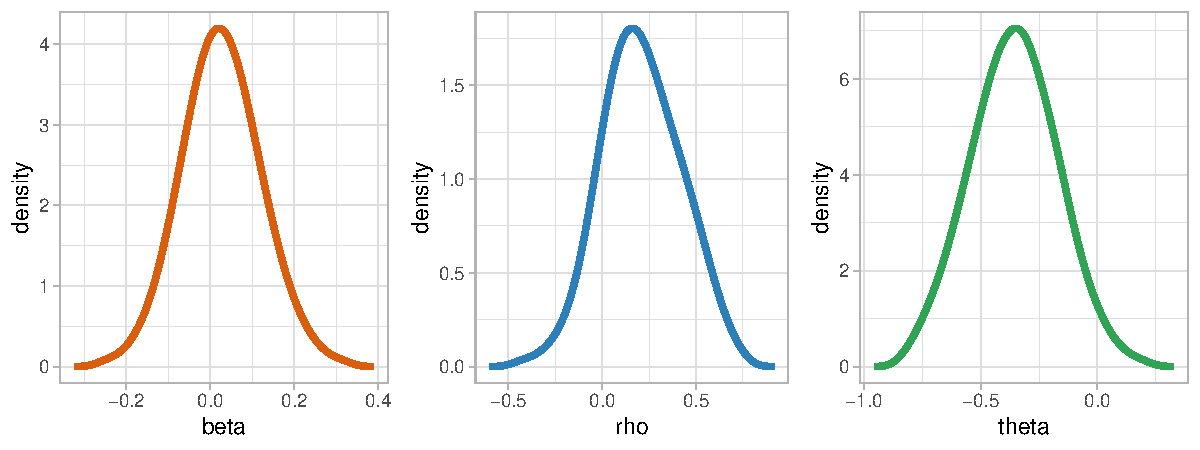
\includegraphics[width=1.0\textwidth]{figures/kernel_densities.pdf}
% %     \end{center}
% %     \caption*{  \scriptsize Note: Posterior mean of the kernel density for the cross-section of $\theta_i$ (left panel), $\rho_i$ (middle panel), and $\theta_i$ (right panel).\par} 
% %     \vspace{0.0cm}
% %     \label{fig: kernel_estimates}
% % \end{figure}
% The disagreement index (DI) has two components: First, the cross-sectional dispersion in $\theta_i$. 
% Second, the absolute value of current aggregate earnings growth, $|\Delta e_t|$. If all analysts agree on the persistence of aggregate earnings growth, such that $\overline{\sigma}[\theta_i] = 0$, then the DI would equal to zero. In turn,given that $\Delta e_t$ has been already de-meaned, $|\Delta e_t|$ captures the distance of aggregate earnings growth to the mean. 
% If aggregate earnings growth is at its average value, $|\Delta e_t| = 0$, there is no disagreement. Thus, the DI depends on the interaction deviations from mean of aggregate earnings and the underlying disagreement about the speed of reversal.  

% The left panel of Figure \ref{fig: DI_turnover_time_series} shows the time series of DI. Disagreement is low during expansions, but spikes in recessions, the periods where earnings growth deviates most from mean. 

% \paragraph{Turnover.} Theories of belief disagreement theories relate to stock-market turnover. We relate the value-weighted stock-market turnover with the DI.
% % \footnote{For a discussion of turnover as a measure of trading volume and its connection with standard portfolio theory, see \citet{lo2010stock}.} 
% \footnote{We measure the stock turnover - shares traded divided by shares outstanding---for individual securities on the New York and American Stock Exchanges from January 1977  to December 2021. We measure turnover at the quarterly frequency and compute an aggregate turnover measure using a value-weighted average (similar results are obtained by using an equal-weight measure).}
% The right panel of Figure \ref{fig: DI_turnover_time_series} shows the time series of turnover. Turnover increased significantly over time, but more importantly for our purposes, shows an important countercyclical behavior.
% % potentially reflecting an increase in market participation, 
% %, as shown by the difference between the turnover and its HP-filtered trend.

% \begin{figure}[t!]
%     \caption{Time series of the disagreement index and stock market turnover}
%     \begin{center}
%             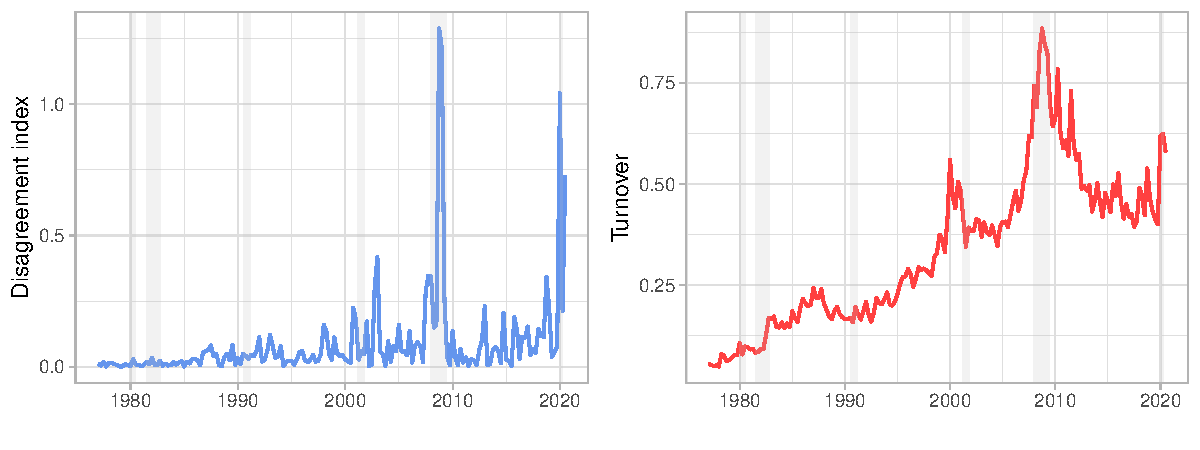
\includegraphics[width=1.0\textwidth]{figures/DI_turnover_time_series.pdf}
%     \end{center}
%     \caption*{  \scriptsize Note: Left panel shows the time series of the disagreement index and the right panel shows the time-series of stock market turnover. The smooth line in the right panel is the HP-filter trend of turnover. The vertical bars represent NBER recessions.\par} 
%     \vspace{0.0cm}
%     \label{fig: DI_turnover_time_series}
% \end{figure}

% Next, we compare the DI with turnover. 
% Table \ref{tab:reg_turnover_DI} shows the result of a time-series regression of turnover against the DI. As shown in Figure \ref{fig: DI_turnover_time_series}, the disagreement DI features outliers particularly during recessions. We thus exclude observations where the DI is below the $2.5\%$ percentile or above the $97.5\%$ percentile. 
% Column (1) shows a strong statistically significant correlation between DI and turnover.
% % SB: ---we compute Newey-West standard-errors with four lags. To bottom of table!
% If the disagreement index increases from the $25\%$ percentile value to its $75\%$ percentile value, turnover increases
% % by $8.0$ percentage points, an increase of 
% by almost $30\%$. 
% Column (2) shows that turnover responds particularly strongly to the DI during downturns. 
% We add an interaction of the DI with a dummy for NBER recessions and find that the coefficient is positive and statistically significant; its magnitude is economically large, the response of turnover to the DI is $70\%$ larger in recessions. 
% Column (3) tests for a nonlinear relationship: we introduce a quadratic term, again excluding outliers. The quadratic term is non significant. %, consistent with a linear relationship---see also Figure \ref{fig: DI_turnover_scatter}, which shows the scatterplot of turnover and the disagreement index for this sample.
% However, Column (4) performs the same non-linear regression but including outliers. In this case, the quadratic term becomes statistically significant, again indicating that the outliers also capture increased disagreement during downturns. 
% % The magnitude of the linear terms in the regressions is similar in all cases. 

% We conclude this analysis a remark: 
% \begin{remark}
% The DI is strongly correlated with turnover, but more so in crises. 
% \end{remark}
% In the theory section, connect this evidence with the predictions of different belief models.

% \begin{table}[t!]
%     	\centering
%     	\caption{Regression of turnover on disagreement index}
%  	\begin{tabular}{lcccc}
%    \tabularnewline \midrule \midrule
%    Dependent Variable: & \multicolumn{4}{c}{$turnover$}\\
%    Model:         & (1)            & (2)            & (3) & (4)\\  
%    \midrule
%    \emph{Variables}\\
%    (Intercept)    & 0.258$^{***}$ & 0.262$^{***}$ & 0.242$^{***}$ & 0.255$^{***}$\\   
%                   & (0.034)      & (0.042)       & (0.044)       & (0.037)\\   
%    $DI$             & 1.239$^{***}$  & 1.066$^{**}$  & 1.798$^{**}$  & 1.260$^{***}$\\   
%                   & (0.228)       & (0.628)       & (0.628)       & (0.290)\\   
%    $DI \times $ recession   &      & 0.742$^{**}$  &          & \\   
%                   &                & (0.253)        &         & \\       
%    $DI^2$            &             &          & -2.068         & -0.688$^{**}$\\   
%                   &                &         & (1.692)        & (0.209)\\   
   
%    \midrule
%    \emph{Fit statistics}\\
%    Observations   & 165            & 165            & 165            & 175\\  
%    R$^2$          & 0.24084        & 0.26430        & 0.24786        & 0.30386\\  
%    Adjusted R$^2$ & 0.23618        & 0.25522        & 0.23857        & 0.29576\\  
%    \midrule \midrule
%    \multicolumn{4}{l}{\emph{Newey-West standard-errors in parentheses (4 lags)}}\\
%    \multicolumn{4}{l}{\emph{Signif. Codes: ***: 0.01, **: 0.05, *: 0.1}}\\
% \end{tabular}
% \caption*{  \scriptsize Note: Columns (1) and (2) .\par} 
%     \label{tab:reg_turnover_DI}
% \end{table}





%%%%%%%%%%%%%%%%%%%%%%%%%%%%%%%%%%%%%%%%%%%%%%%%%%%%%%%%%%%%%%%%%%%%%%%%%%%%%%%%%%%%%%%%%%%%%%%



% \begin{figure}[t!]
%     \caption{Scatterplot of the disagreement index and stock market turnover}
%     \begin{center}
%             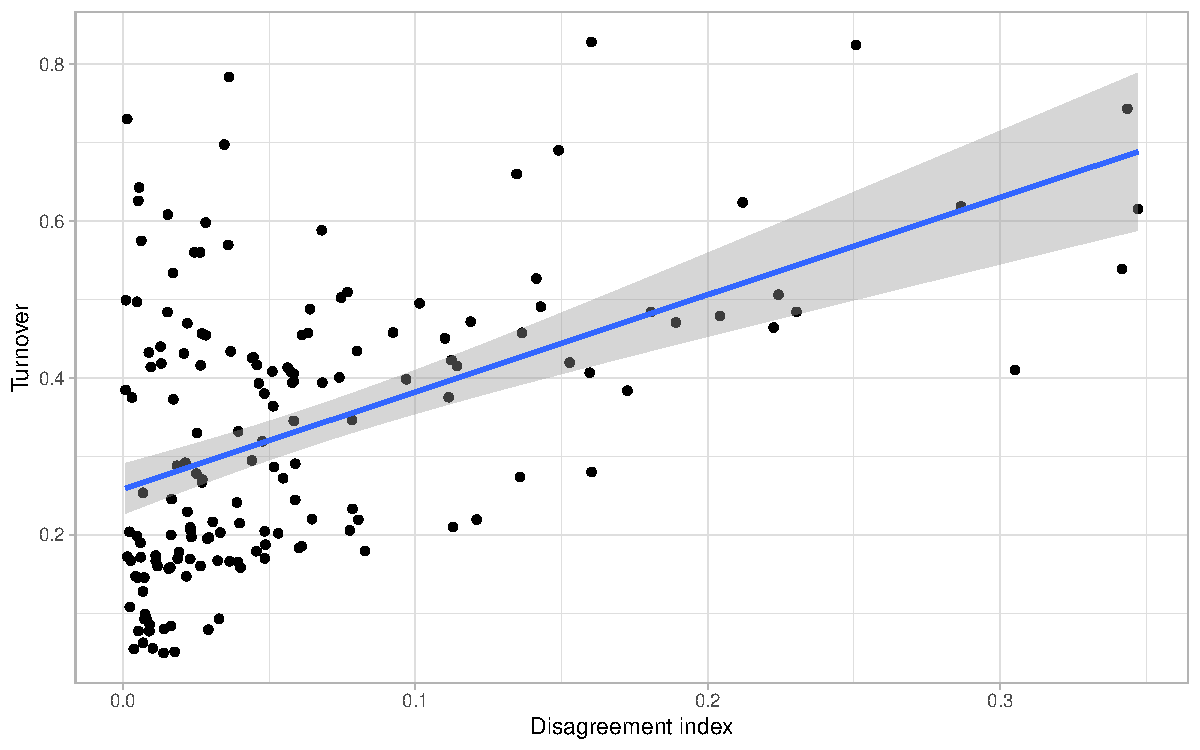
\includegraphics[width=0.8\textwidth]{figures/DI_turnover_scatter.pdf}
%     \end{center}
% %    \caption*{  \scriptsize Note: .\par} 
%     \vspace{0.0cm}
%     \label{fig: DI_turnover_scatter}
%     \caption*{  \scriptsize Note: Scatterplot of disagreement index and turnover for a sample without outliers.\par} 
% \end{figure}



% \paragraph{Connecting with the Turnover Evidence.}
% It is convenient to express heterogeneity in beliefs, $p_{ss}^i$, in terms of heterogeneity in the perceived \textit{persistence} of fundamentals. Assuming investors agree on the unconditional mean of $x_t$, $\overline{x}$, we can write $\mathbb{E}_{i,t}[x_{t+1}] - \overline{x} = \theta_i (x_t - \overline{x})$, where $\theta_i$ is a function of $p_{ss'}^i$.
% % We can recast beliefs about $p_{ss}^i$ into beliefs about mean reversion rates in earning growth, $\theta^i$---as estimated in Section \ref{sec:quantitative}. 
% The following corollary shows heterogeneous beliefs lead to larger turnover rates as the economy switches from booms to recessions.
% \begin{corollary}\label{cor: turnover} Suppose investors agree on the unconditional mean of $x_t$, i.e. $p_{LH}^i / p_{HL}^i = \overline{p}_H / \overline{p}_L$ and that the following condition is satisfied: $p_{ss'}^* = \overline{p}_H = \frac{1}{2}$. Turnover as the economy switches from $s$ to $s'$ is given by
% \begin{equation}
%     \tau(X,H,L;\epsilon) = \frac{\zeta(s,s')}{2}\sum_{i=1}^I \eta_i |\theta_i - \theta(X)| + \mathcal{O}(\epsilon^2),
% \end{equation}
% where
% \begin{equation*}
%     \zeta(s,s') \equiv \left\{ 
%     \begin{matrix}
%     \kappa_\omega + 1, \qquad & \text{if } $s = H$ \text{ and } $s' = L$\\
%     |\kappa_\omega - 1|, \qquad & \text{if } $s = L$ \text{ and } $s'  = H$\\
%     1, \qquad & \text{if } $s = s'$
%     \end{matrix}
%     \right. 
% \end{equation*}
% \end{corollary}
% % The assumption $p_{ss'}^* = \overline{p}_H = \frac{1}{2}$ is made only to simplify the presentation. The general case is considered in the appendix.
%  The key message from Corollary \ref{cor: turnover} is that turnover increases in belief dispersion and, furthermore, that the effect is more pronounced during busts. 
% Both predictions are in line with the evidence discussed in Section \ref{app_disagreement_evidence}. The assumption of rank-alternating beliefs is important to obtain this asymmetric effect. 
% If investors have rank-preserving beliefs, where they are equally optimistic or pessimistic in both states, so $\tilde{\delta}_{s'H}^i = \tilde{\delta}_{sH}^i $ even for $s'\neq s$, then the change-in-beliefs effect will be equal to zero and we would not obtain a stronger response of turnover to disagreement during bad times. Therefore, rank-alternating beliefs are key to capturing the dynamics of stock market turnover. 

% Our taxonomy also has implications for trading dynamics.
% As is typical in models of belief heterogeneity, trading volume increases with the level of belief disagreement.
% More importantly, Appendix~\ref{app:volume} shows that the relationship between trading volume and belief disagreement is amplified during economic downturns under \textit{rank-alternating} beliefs, not under \textit{rank-preserving} beliefs. 
% The intuition is as follows: optimistic investors lose wealth and rebalance their portfolios by selling shares when the economy enters a recession. 
% If their beliefs are rank-alternating, they also become pessimistic, which induces additional selling, further increasing trading volume.
% % Intuitively, optimistic investors lose wealth as the economy switches to the bad state, so they rebalance their portfolios by selling shares. 
% % If they have rank-alternating beliefs, they also become pessimistic, leading to an additional selling of shares, further increasing trading volume.
% Appendix~\ref{app:belief_heterogeneity_estimation} provides empirical support for this prediction. 
% We find that not only does stock market turnover rise with belief disagreement, but this relationship also strengthens during recessions, consistent with the predictions under rank-alternating beliefs.


\section{Quantitative analysis}\label{sec:quantitative}

We now consider the quantitative implications. We extend the baseline formulation in Section \ref{sec:environment.sec}: First, productivity growth $x_t$ now follows a more general process. This is necessary to capture the empirical patterns of dividend growth. Second, we introduce a force that induces a non-degenerate stationary wealth distribution. A force like this is needed so that belief heterogeneity survives in the ergodic distribution of the model.
We do so through Uzawa endogenous discounting for convenience. This specific approach is not indispensable; we can obtain non-degeneracy through birth-death processes for example.  

\paragraph{Belief process with a continuum of states.}

We start by specifying a continuous Markov process for $x_t$ under both objective and subjective beliefs. 
Let $\hat{x}_{t} \equiv \log x_t $ denote log aggregate productivity growth. Under the objective measure, $\hat{x}_t$ follows:
\begin{equation}\label{eq: x_objective}
    \hat{x}_{t+1} = \mu_x +  \sigma_x \epsilon_{x,t+1}.
\end{equation}
where $\epsilon_{x,t+1} \overset{\text{iid}}{\sim} N(0,1)$. Thus, productivity growth is iid under the objective measure. 

In turn, subjective beliefs about $\hat{x}_t$ for household $i \in \mathcal{I} $ are given by:
\begin{align}
    \hat{x}_{t+1} &= \mu_{x,i} + \rho_{x,i} (\hat{x}_{t} - \mu_{x,i}) + v_{i,t} + \sigma_{x,i} \epsilon_{x,i,t+1},
\end{align}
where $\epsilon_{x,i,t+1} \overset{\text{iid}}{\sim} N(0,1)$. 
Beliefs deviate from the process \eqref{eq: x_objective} in two critical ways:
First, the subjective conditional expectation responds to current productivity growth $\hat{x}_t$. This dimension is important to allow 
households to over- or under-react to past information, consistent with Fact 2 in Section \ref{sec:facts.sec}. Overreaction is controlled by $\rho_{x,i}$. For instance, a positive $\rho_{x,i}$ implies the household overreacts to productivity news, given our assumption that productivity growth is iid under the objective measure. 

Second, beliefs are also exposed to a persistent \textit{sentiment shock} $v_{t}$, which evolve according to
\begin{equation}
    v_{i,t+1} = \rho_{v,i} v_{i,t} + \sigma_{v,i} \epsilon_{v,i,t+1}
\end{equation}
where $\epsilon_{v,i,t+1} \overset{\text{iid}}{\sim} N(0,1)$, and $\epsilon_{v,i,t}$ and $\epsilon_{x,i,t}$ are uncorrelated. 

The sentiment is independent of TFP growth. Thus, this shock leads to fluctuations in the degree of optimism unrelated to fundamentals. Introducing this shock is necessary to quantitatively match the volatility of subjective TFP growth expectations relative to the objective one---Fact 1 in Section \ref{sec:facts.sec}. While extrapolation, through higher values of $\rho_{x,i}$, increases the volatility of subjective expectations, it is insufficient, so the sentiment is needed. 

We note that the belief system in this section is a hybrid of the one in our taxonomy. It encompasses both extrapolation and time-dependent optimism through sentiment shock. We let the survey data discipline the strength of each force. 
% Investors' beliefs deviate from the objective process for $\hat{x}_{t+1}$ in two important ways.
% First, investors disagree about the persistence of states. Some investors believe that positive shocks persist, $\theta_i > 0$, while others believe that shocks revert, $\rho_{x,i} < 0$. 
% Second, beliefs are subject to a common sentiment shock, $v_t$. 
% We impose that the unconditional variance of $\hat{x}_t$ under subjective beliefs coincides with the actual unconditional variance, $Var_i[\hat{x}_t] = \sigma_x^2$. 
% Relative to the objective measure, sentiment shocks cause a larger fraction of the variation of $\hat{x}$ to be attributed to movements in expectations. 
% Sentiment shocks allow us to reproduce the observed volatility of expectations in the data. 
% We further assume that investors agree on the transition probabilities of $w_{t+1}$ and observe its current value. Thus, investors understand that earnings have fat tail. Hence, the only source of disagreement is the persistence of shocks $\theta_i$. 

% Appendix \ref{sec:discretization}  discusses the discretization of the process for $\hat{x}_t$. 
% The discretization provides a state space with dimension $S$  for $x_t$, so $x_t \in \mathcal{X}= \{x^1, x^2, \ldots, x^S\}$,  and transition probabilities $\{p_{ss'}^i\}$, for $s, s' \in \mathcal{S} = \{1,2, \ldots, S\}$. Our discretization implies that the grid $\mathcal{X}$ is the same for all investors, so they agree on the state $s$, but they disagree on the transition probabilities $p_{ss'}^i$.

\paragraph{Endogenous discounting.} 
To ensure the wealth distribution is stationary, we assume that households' subjective discount rate responds to their consumption share:
\begin{equation}
    \beta_{i,t} = \beta e^{\kappa \left(1 - \frac{\mu_i \tilde{C}_{i,t}}{\tilde{Y}_t}\right)}. 
\end{equation}
This assumption, a form of \citet{uzawa2017time} preferences, implies that households' marginal propensity to consume increases with their share of consumption, ensuring that no investor type concentrates all the wealth asymptotically.  Following \citet{schmitt2003closing}, we assume that $\beta_{i,t}$ depends on the average consumption share of type-$i$ households, so households take the process for $\beta_{i,t}$ as given.\footnote{This mechanism is often used in small open-economy models to ensure a stationary distribution of external debt.}

% \paragraph{Model solution.} We describe the model characterization with a continuum of states and Uzawa preferences in Appendix~\ref{app:numerical_solution}. 
% Previous results are essentially unchanged. 
% As in the binary case, an exact closed-form solution is unavailable away from log preferences.
% We compute the solution using a third-order perturbation around the non-stochastic steady state, following, e.g., \citet{van2012term}. 
% A third-order perturbation is indispensable to capture time variation in expected returns.\footnote{For a discussion of the accuracy of the perturbation method, see \citealt{caldara2012computing}.} 
% Simulations are performed using a pruned state-space representation of the higher-order solution to avoid spurious explosive dynamics induced by truncation of the perturbation expansion (see \citealt{andreasen2018pruned}).
\paragraph{Model solution.}
Appendix~\ref{app:numerical_solution} describes the characterization of the model with a continuum of states and Uzawa preferences. The qualitative mechanisms discussed in the binary-state case carry over to this richer environment.
Away from log preferences, no closed-form solution is available. We therefore solve the model using a third-order perturbation around the non-stochastic steady state, following, for example, \citet{van2012term}. A third-order approximation is necessary to generate time variation in risk premia and expected returns.\footnote{For evidence on the accuracy of higher-order perturbation methods, see \citealt{caldara2012computing}.}
Simulations are based on the pruned state-space representation of the higher-order solution (see \citealt{andreasen2018pruned}).


\paragraph{Calibration.} \q{CaliStandardBlock}{We use the following calibration, where parameters are expressed in quarterly terms. Preferences and technology parameters are standard.  \textit{Preferences}: We set $\beta = 0.978$ to match an unconditional annualized risk-free rate of $1\%$. 
The risk aversion is set to $\gamma = 10.0$ and the EIS to $\psi = 2.0$, typical values in the macro-finance literature. 
We choose the labor disutility parameter $\xi$ to normalize the average hours to 1 and set the Frish elasticity to one, $\nu = 1$, a standard value in the literature.
\textit{Technology:} We set $\alpha = 0.66$ and choose $\mu_x$ and $\sigma_x$ to match the average and standard deviation of annual consumption growth of $2.1\%$ and $2.7\%$, respectively.} 

\q{CaliBeliefs}{The calibration of the belief processes is novel. 
\textit{Beliefs:} We focus on the case $I = 2$, and assume that households of type $i = 2$ have rational beliefs, which allows for some rational agents in the environment. We set $\mu_{x,1} = \mu_x$ and $\sigma_{x,1} = \sigma_x$, so households agree on the mean and conditional volatility of productivity growth. 
We set $\mu_2 = 0.1$, so the fraction of rational agents in the population is $10\%$, consistent with the fact that average beliefs in surveys of households and analysts show substantial deviations from rational expectations. 
We set $\rho_{v,1}$ and $\sigma_{v,1}$ to match the persistence of subjective dividend growth and the share of variance explained by movements in expectations, based on estimations of \citet{de_la_o_subjective_2021}.
In turn, we set $\rho_{x,1}$ to match the correlation between subjective expectations and current productivity growth observed in the data. This calibration is agnostic about the relevant belief system: the subjective belief moments pin down these parameters, determining whether non-rational beliefs are extrapolation or rank-preserving. Finally, we set $\kappa = 0.5\%$, consistent with the mean-reversion in consumption shares in \citet{garleanu2015young}.} 

\subsection{Biases in productivity growth expectations}
\label{sec:biases_expectations.sec}
\q{ProdExpectationI}{
In the model, investors hold distorted beliefs about productivity growth.
These distortions propagate to other variables --- such as dividends and returns ---
through the likelihood-ratio representation:
\begin{equation}
    \mathbb{E}_{i,t}[Z_{t+1}]
    =
    \mathbb{E}_t[\ell_{i,t+1} Z_{t+1}],
\end{equation}
where $\ell_{i,t+1}$ is the likelihood-ratio between subjective and objective beliefs.
Hence, a single distortion in productivity growth beliefs induces distortions
in expectations of all equilibrium objects.\footnote{
\citet{cui_subjective_2024} estimate an empirical counterpart to the likelihood ratio
and show that it explains a large fraction of cross-sectional variation in survey expectations.
}

It is therefore important to verify that the model is consistent with the empirical
properties of subjective productivity growth expectations.

\paragraph{Coibion--Gorodnichenko regressions.}

We assess this using Coibion--Gorodnichenko (CG) regressions
\citep{coibion2015information}, which test for systematic forecast biases by regressing
forecast errors on forecast revisions:
\begin{equation}
    \Delta prod_{t+h} - \mathbb{E}_{i,t}[\Delta prod_{t+h}]
    =
    c + \beta_{CG}
    \left(
        \mathbb{E}_{i,t}[\Delta prod_{t+h}]
        -
        \mathbb{E}_{i,t-1}[\Delta prod_{t+h}]
    \right)
    + u_{t+h}.
\end{equation}

Under full-information rational expectations, $\beta_{CG}=0$.
A negative estimate indicates over-extrapolation: agents revise forecasts too strongly
in the direction of recent news.

\paragraph{Empirical implementation.}

As direct survey data on TFP growth expectations are limited, we consider two alternative measures of productivity growth
using quarterly data from the Survey of Professional Forecasters (SPF):
\begin{align}
    \Delta prod^{LP}_{t+1} &= \Delta \hat y_{t+1} - \Delta \hat n_{t+1}, \\
    \Delta prod^{TFP}_{t+1} &= \Delta \hat y_{t+1} - \alpha\,\Delta \hat n_{t+1},
\end{align}
where $\Delta \hat y$ is GDP growth, $\Delta \hat n$ is employment growth, and we set $\alpha=2/3$.

The first measure corresponds to labor productivity growth, and the second is a TFP proxy consistent with how TFP growth is defined in the model.
Table~\ref{tab:cg_productivity_h1} reports the results.
For labor productivity, we estimate
$\hat{\beta}_{CG} = -0.63$,
and for the TFP proxy,
$\hat{\beta}_{CG} = -0.50$,
both statistically significant.

\paragraph{Model comparison.}

We perform the same CG regression using simulated data from the calibrated model.
The model implies
\[
\hat{\beta}_{CG}^{\text{model}} = -0.695.
\]
This value is very close to the empirical estimate for labor productivity
and lies within one standard error of the estimate for the TFP proxy.
}
\begin{table}[!t]
    \centering
    \caption{Coibion--Gorodnichenko Regressions for Productivity Measures}
    \label{tab:cg_productivity_h1}
    \begin{threeparttable}
    \begin{tabular}{lcc}
    \toprule
     & Labor Productivity & TFP Proxy \\
    \midrule
    Forecast revision coefficient $\beta_{CG}$ 
    & -0.63$^{***}$ 
    & -0.50$^{**}$ \\
    & (0.030) & (0.198) \\
    Constant 
    & -0.15 
    & -0.25 \\
    & (0.289) & (0.259) \\
    \midrule
    Observations 
    & 86 & 86 \\
    $R^2$ 
    & 0.3697 & 0.0579 \\
    Adj. $R^2$ 
    & 0.3622 & 0.0467 \\
    \bottomrule
    \end{tabular}
    \begin{tablenotes}[flushleft]
    \footnotesize
    \item Notes: Each column reports OLS estimates of
    $\text{FE}_t = c + \beta \,\text{Revision}_t + u_t$, where $h=1$ quarter.
    Reported standard errors (in parentheses) are Newey--West HAC with lag 4.
    Labor productivity uses $\Delta y - \Delta n$.
    TFP proxy uses $\Delta y - \alpha \Delta n$ with $\alpha=2/3$.
    Sample: 2004Q1--2025Q2.
    Significance: $^{*} p<0.10$, $^{**} p<0.05$, $^{***} p<0.01$ (based on HAC $p$-values).
    \end{tablenotes}
    \end{threeparttable}
    \end{table}

    
    \q{ProdExpectationII}{
    These results support the model's mechanism.
    The same distortions that drive endogenous movements in labor demand
    and risk premia also generate empirically realistic forecast biases
    in productivity growth.
    
    Overall, even though the model is not directly calibrated to productivity-expectations moments, it reproduces the key bias pattern observed in the data.
    }

\subsection{Unconditional moments}\label{sec:unconditional_moments.sec}

Next, we study the model's ability to match unconditional moments. 
To isolate the role of each ingredient, we start from a stripped-down version of the model and progressively add features until we reach the complete model. 
This progression allows us to discuss the role of each ingredient in the model. Table \ref{tab:uncond_moments} presents the results under each formulation.
The table also reports $\pm 2$ standard-error intervals for the data moments.

\q{QuantTable}{
% In preamble:
% \usepackage{booktabs}
% \usepackage{graphicx}

\begin{table}[t]
    \centering
    \caption{Unconditional moments}
    \label{tab:uncond_moments}
    \resizebox{\textwidth}{!}{%
    \renewcommand{\arraystretch}{1.75} % try 1.15-1.3
    \begin{tabular}{@{}lcccccccccccc@{}}
    \toprule\toprule
    & \multicolumn{4}{c}{\textbf{Rational Beliefs}}
    & \multicolumn{6}{c}{\textbf{Subjective Beliefs}}
    & \multicolumn{2}{c}{} \\
    \cmidrule(lr){2-5}\cmidrule(lr){6-11}
    & \multicolumn{2}{c}{\textbf{Endowment}}
    & \multicolumn{2}{c}{\textbf{Production}}
    & \multicolumn{2}{c}{\textbf{Homogeneous}}
    & \multicolumn{2}{c}{\textbf{Heterogeneous}}
    & \multicolumn{2}{c}{\textbf{High elast.}}
    & \multicolumn{2}{c}{\textbf{Data (\(\pm 2\) s.e.)}} \\
    \cmidrule(lr){2-3}\cmidrule(lr){4-5}\cmidrule(lr){6-7}\cmidrule(lr){8-9}\cmidrule(lr){10-11}\cmidrule(lr){12-13}
    \textbf{Variables}
    & \textbf{Mean} & \textbf{Std}
    & \textbf{Mean} & \textbf{Std}
    & \textbf{Mean} & \textbf{Std}
    & \textbf{Mean} & \textbf{Std}
    & \textbf{Mean} & \textbf{Std}
    & \textbf{Mean} & \textbf{Std} \\
    \midrule
    Interest rate           & 10.2 & 0.0 & 10.0 & 0.7 & 10.1 & 1.3 & 1.3 & 6.4 & 1.2 & 6.4 & [0.6, 3.0] & [3.7, 6.0] \\
    Excess returns (equity) &  0.7 & 2.7 & 1.2 & 7.2 & 1.2 & 8.3 & 5.6 &16.8 & 5.7 &16.7 & [3.5, 9.3] & [15.6, 21.4] \\
    \midrule
    Consumption growth      &  2.1 & 2.7 & 2.1 & 2.7 & 2.1 & 2.8 & 2.1 & 2.8 & 2.1 & 3.0 & [1.2, 3.1] & [2.0, 3.4] \\
    Dividend growth         &  2.1 & 2.7 & 2.1 & 9.3 & 2.1 &10.0 & 2.1 &10.0 & 2.1 & 9.8 & [-0.3, 3.4] & [6.9, 11.2] \\
    \midrule
    Log hours               &  0.0 & 0.0 &  0.2 & 0.0 &  0.2 & 1.3 &  0.2 & 1.2 & 0.6 & 1.9 & --  & [1.7, 2.7] \\
    \bottomrule\bottomrule
    \end{tabular}%
    }
    \vspace{0.35em}
    \parbox{\textwidth}{\scriptsize
    \vspace{0.7em}
    \textit{Note:} The table reports annualized unconditional moments in percentage points. Column 1 is the endowment benchmark with rational beliefs; Column 2 adds production with labor chosen in advance under rational beliefs; Column 3 is the homogeneous-beliefs version of the production model; Column 4 is the heterogeneous-beliefs benchmark calibration; Column 5 is the high-labor-elasticity robustness. The data columns report point estimate \(\pm 2\) bootstrap standard errors. Detailed data construction, sample windows, and bootstrap methodology are provided in the Data Appendix (Appendix~\ref{app:data_table5_moments}).
    }
    \end{table}

    
% \begin{table}[t]
% \centering
% \footnotesize
% \setlength{\tabcolsep}{2.5pt}
% \begin{threeparttable}
% \caption{Unconditional moments}
% \label{tab:uncond_moments}

% \begin{tabular}{@{}l*{12}{c}@{}}
% \toprule\toprule
% & \multicolumn{4}{c}{\textbf{Rational Beliefs}}
% & \multicolumn{6}{c}{\textbf{Subjective Beliefs}}
% & \multicolumn{2}{c}{} \\
% \cmidrule(lr){2-5}\cmidrule(lr){6-11}
% & \multicolumn{2}{c}{\textbf{Endowment}}
% & \multicolumn{2}{c}{\textbf{Production}}
% & \multicolumn{2}{c}{\textbf{Homogeneous}}
% & \multicolumn{2}{c}{\textbf{Heterogeneous}}
% & \multicolumn{2}{c}{\textbf{High elast.}}
% & \multicolumn{2}{c}{\textbf{Data}} \\
% \cmidrule(lr){2-3}\cmidrule(lr){4-5}\cmidrule(lr){6-7}\cmidrule(lr){8-9}\cmidrule(lr){10-11}\cmidrule(lr){12-13}
% \textbf{Variables}
% & \multicolumn{1}{c}{\textbf{Mean}} & \multicolumn{1}{c}{\textbf{Std}}
% & \multicolumn{1}{c}{\textbf{Mean}} & \multicolumn{1}{c}{\textbf{Std}}
% & \multicolumn{1}{c}{\textbf{Mean}} & \multicolumn{1}{c}{\textbf{Std}}
% & \multicolumn{1}{c}{\textbf{Mean}} & \multicolumn{1}{c}{\textbf{Std}}
% & \multicolumn{1}{c}{\textbf{Mean}} & \multicolumn{1}{c}{\textbf{Std}}
% & \multicolumn{1}{c}{\textbf{Mean}} & \multicolumn{1}{c}{\textbf{Std}} \\
% \midrule
% Interest rate           & 10.0 & 0.0 & 9.7 & 0.7 & 9.7 & 1.4 & 1.0 & 6.4 & 0.8 & 6.5 & 0.8 & 5.7 \\
% Excess Returns (equity) &  0.9 & 3.0 & 1.4 & 7.9 & 1.5 & 9.3 & 5.8 &17.3 & 6.0 &17.1 & 6.2 &16.5 \\
% \midrule
% Consumption growth      &  1.8 & 3.0 & 1.8 & 3.0 & 1.8 & 3.1 & 1.8 & 3.1 & 1.8 & 3.3 & 1.8 & 3.0 \\
% Dividend growth         &  1.8 & 3.0 & 1.8 &10.3 & 1.8 &11.2 & 1.8 &11.1 & 1.8 &10.9 & \multicolumn{1}{c}{--} &11.5 \\
% \midrule
% Log hours               &  0.0 & 0.0 &-0.1 & 0.0 &-0.1 & 1.5 &-0.1 & 1.3 & 0.0 & 2.1 & \multicolumn{1}{c}{--} & 2.4 \\
% \bottomrule\bottomrule
% \end{tabular}

% \begin{tablenotes}[flushleft]
% \scriptsize
% \item Note: ...
% \end{tablenotes}
% \end{threeparttable}
% \end{table}



% \begin{table}[t!]
% \resizebox{\textwidth}{!}{
% \begin{tabular}{@{}l||ll|ll||ll|ll|ll||ll@{}} \toprule\toprule
%                          & \multicolumn{4}{c||}{\textbf{Rational Beliefs}}                                                         & \multicolumn{6}{c||}{\textbf{Subjective Beliefs}}                    & \multicolumn{2}{c}{} \\
%                          & \multicolumn{2}{c|}{\textbf{Endowment}} & \multicolumn{2}{c||}{\textbf{Production}} & \multicolumn{2}{c|}{\textbf{Homogeneous}} & \multicolumn{2}{c|}{\textbf{Heteregeneous}} & \multicolumn{2}{c||}{\textbf{High elast.}} & \multicolumn{2}{c}{\textbf{Data}}          \\ \midrule
%                          &&&&&&&&&&&\\[-0.7em]
% \textbf{Variables}       & \textbf{Mean}   & \textbf{Std}   & \textbf{Mean}   & \textbf{Std}   & \textbf{Mean}   & \textbf{Std}   & \textbf{Mean}   & \textbf{Std}   & \textbf{Mean}   & \textbf{Std}   & \textbf{Mean}        & \textbf{Std}       \\ 
% &&&&&&&&&&&\\[-0.7em]
% \midrule
% &&&&&&&&&&&\\[-0.7em] 
% Interest rate            & 10.0            & 0.0              & 9.7            & 0.7           & 9.7            & 1.4           & 1.0            & 6.4           & 0.8            & 6.5           & 0.8                 & 5.7               \\
% &&&&&&&&&&&\\[-0.7em]
% Excess Returns (equity)  & 0.9            & 3.0            & 1.4            & 7.9           & 1.5            & 9.3           & 5.8             & 17.3           & 6.0            & 17.1           & 6.2                 & 16.5              \\
% &&&&&&&&&&&\\[-0.7em] \midrule
% &&&&&&&&&&&\\[-0.7em] 
% Consumption growth       & 1.8               & 3.0           & 1.8            & 3.0           & 1.8            & 3.1            & 1.8            & 3.1           & 1.8            & 3.3           & 1.8                 & 3.0               \\
% &&&&&&&&&&&\\[-0.7em]
% Dividend growth          & 1.8               & 3.0           & 1.8            & 10.3           & 1.8            & 11.2           & 1.8            & 11.1           & 1.8            & 10.9            & -                 & 11.5                \\
% &&&&&&&&&&&\\[-0.7em] \midrule
% &&&&&&&&&&&\\[-0.7em] 
% Log hours                & 0.0               & 0.0              & -0.1           & 0.0              & -0.1           & 1.5              & -0.1           & 1.3           & 0.0           & 2.1           & -                & 2.4               \\ \bottomrule\bottomrule
% \end{tabular}}
% \caption{Unconditional moments}\label{tab:uncond_moments}
% \caption*{  \scriptsize 
%     Note: The table reports annualized unconditional moments in percentage points. 
%     Column 1 shows results for the endowment economy limit with rational beliefs. 
%     Column 2 introduces production with the labor friction. 
%     Column 3 shows the case of homogeneous subjective beliefs. 
%     Column 4 presents the case of heterogeneous beliefs with our calibration.
%     Column 5 presents results for an alternative calibration with a higher labor supply elasticity. 
%     The last set of columns shows the corresponding values in the data.
%     Mean and standard deviation of the interest rate and excess equity returns are from \citet{MP85}. Average consumption growth and the volatility of consumption and dividend growth are from \citet{bansal2004risks}. The standard deviation of total hours is obtained from Table 5 in \citet{ohanian2012aggregate}: total hours include changes in employment and hours worked for 1985Q1:2007Q4. Standard deviations in that paper are reported as deviations from an HP-filter. We convert their quarterly figure to annual rates. \par} 
% \end{table}
}

\q{QuantCol1}{
Column 1 presents the stripped-down version of the model with a single representative rational investor, for which hiring is done after TFP is known and labor supply is inelastic. 
This economy behaves as an Epstein-Zin version of the endowment economy studied by \citet{MP85}. The model fails to generate a sizeable equity premium and excess stock volatility. 
Moreover, without the hiring friction, the volatility of consumption and dividends coincide.
Given that rational beliefs are iid, the price-dividend ratio is constant, so return volatility equals dividend volatility.}
% Given the absence of fluctuations in risk premia, there are no labor fluctuations. 

% The first column presents the stripped-down version with a single representative rational investor, for which hiring is done after TFP is known. 
% As explained in Section \ref{sec:environment.sec}, this economy behaves as an Epstein-Zin version of the endowment economy studied by \citet{MP85}.\footnote{We obtain this limit by making $\alpha$ and $\xi$ go to zero, while $\alpha/\xi$ converges to a positive number. In this case, hours equal a positive constant, but wages and labor disutility are equal to zero.} The model fails to generate a sizeable equity premium and excess stock volatility. Moreover, without hiring risk, the volatility of consumption and dividends coincide, and the price-dividend ratio remains constant. Because the price-dividend ratio is constant, dividend growth exactly equals the excess return on equity, leading to constant risk premia and no endogenous labor fluctuations. 


% This seems like a digression -> let's discuss, they are curious about this in letter.
% Near i.i.d. TFP growth plays a critical role in preventing fluctuations in risk premia, hours, and the price-dividend ratio in this classic setting. This is not true away from iid growth, unlike a setting with log preference where the price-dividend ratio is constant regardless of the dividend growth process. Indeed, under log preferences, the price-dividend ratio is constant even though households supply labor: because the labor share is constant, the price and dividends of stocks are proportional to those of human capital. This indicates that, because we are in a setting with a EIS different from 1, i.i.d. dividend growth places limitations to match asset pricing moments and movements in labor. 

\q{QuantCol2}{Column 2 introduces the timing of hires assumption and the elastic labor supply. 
The operating leverage channel endogenously generates differences in volatility between consumption and dividends in line with the data, even though this is not a targeted moment. 
With iid beliefs, there is no time variation in the price of risk, so the model fails to generate fluctuations in hours.
Moreover, the hiring friction implies that dividend growth follows a mean-reverting process.\footnote{
    For models with mean-reverting dividend process, see e.g. \citet{menzly2004understanding} and \citet{santos2006labor}.} 
Without time-varying risk premia, mean-reversion in dividends causes the price-dividend ratio to negatively correlate with realized returns.
This counterfactual behavior dampens return volatility relative to dividend volatility.}

% Column 2 introduces the timing assumption with elastic labor supply. 
% Hiring risk increases the excess return of equity and its volatility. Moreover, this timing enables us to endogenously generate the differences in volatility between consumption and dividend growth observed in the data. This is because the labor share is no longer constant but countercyclical. Quantitatively, the model matches the volatility of dividends, although this was not a target moment. 

% With pre-set labor, the price-dividend ratio is no longer constant. Dividend growth is not iid even though productivity is: periods with higher than expected TFP lead to an increase in dividends, but because TFP growth is iid, on average, dividends are expected to fall after a surprise increase. Movements in the price-dividend ratio are induced by the timing of hires. 
% In fact, even under log, %where the P/E ratio is constant for non-iid dividend processes, 
% the P/E ratio will move. 
% This is because with log, the P/E ratio of the surplus claim is constant, but the returns of human capital and stocks are no longer correlated.   

% While the timing of hires allows the price-dividend ratio to move, it does so in the opposite direction: high TFP periods are associated with high dividends and low prices, leading to pro-cyclical price-dividend ratios. Furthermore, notice that this version of the model cannot generate any movements in hours. This is because even though risk premia increases with the timing assumption---and hours fall on average, risk-premia is not time-varying, given the assumption of rational expectations and iid productivity growth. 

\q{QuantCol3}{Column 3 considers the role of non-rational beliefs calibrated to match the survey data, while abstracting from differences in beliefs. 
In this case, the model does generate movements in hours, given that subjective beliefs are volatile, consistent with the discussion in Section~\ref{sec:analysis.sec4}. 
However, deviations from rational expectations are insufficient to generate an equity premium and stock return volatility in line with the data. 
Movements in subjective beliefs only attenuate the negative correlation between returns and the price-dividend ratio, so return volatility is still dampened relative to dividend volatility.}   
% Column 3 considers the role of non-rational beliefs calibrated to match the survey data, while abstracting from differences in beliefs. In this case, the model does generates movements in hours, given that subjective beliefs are volatile. However, deviations from rational expectations are not enough to generate an equity premium and stock return volatility in line with the data. Furthermore, the direction of movement in the P/E ratio remains problematic. 

\begin{figure}[t!]
    \centering
            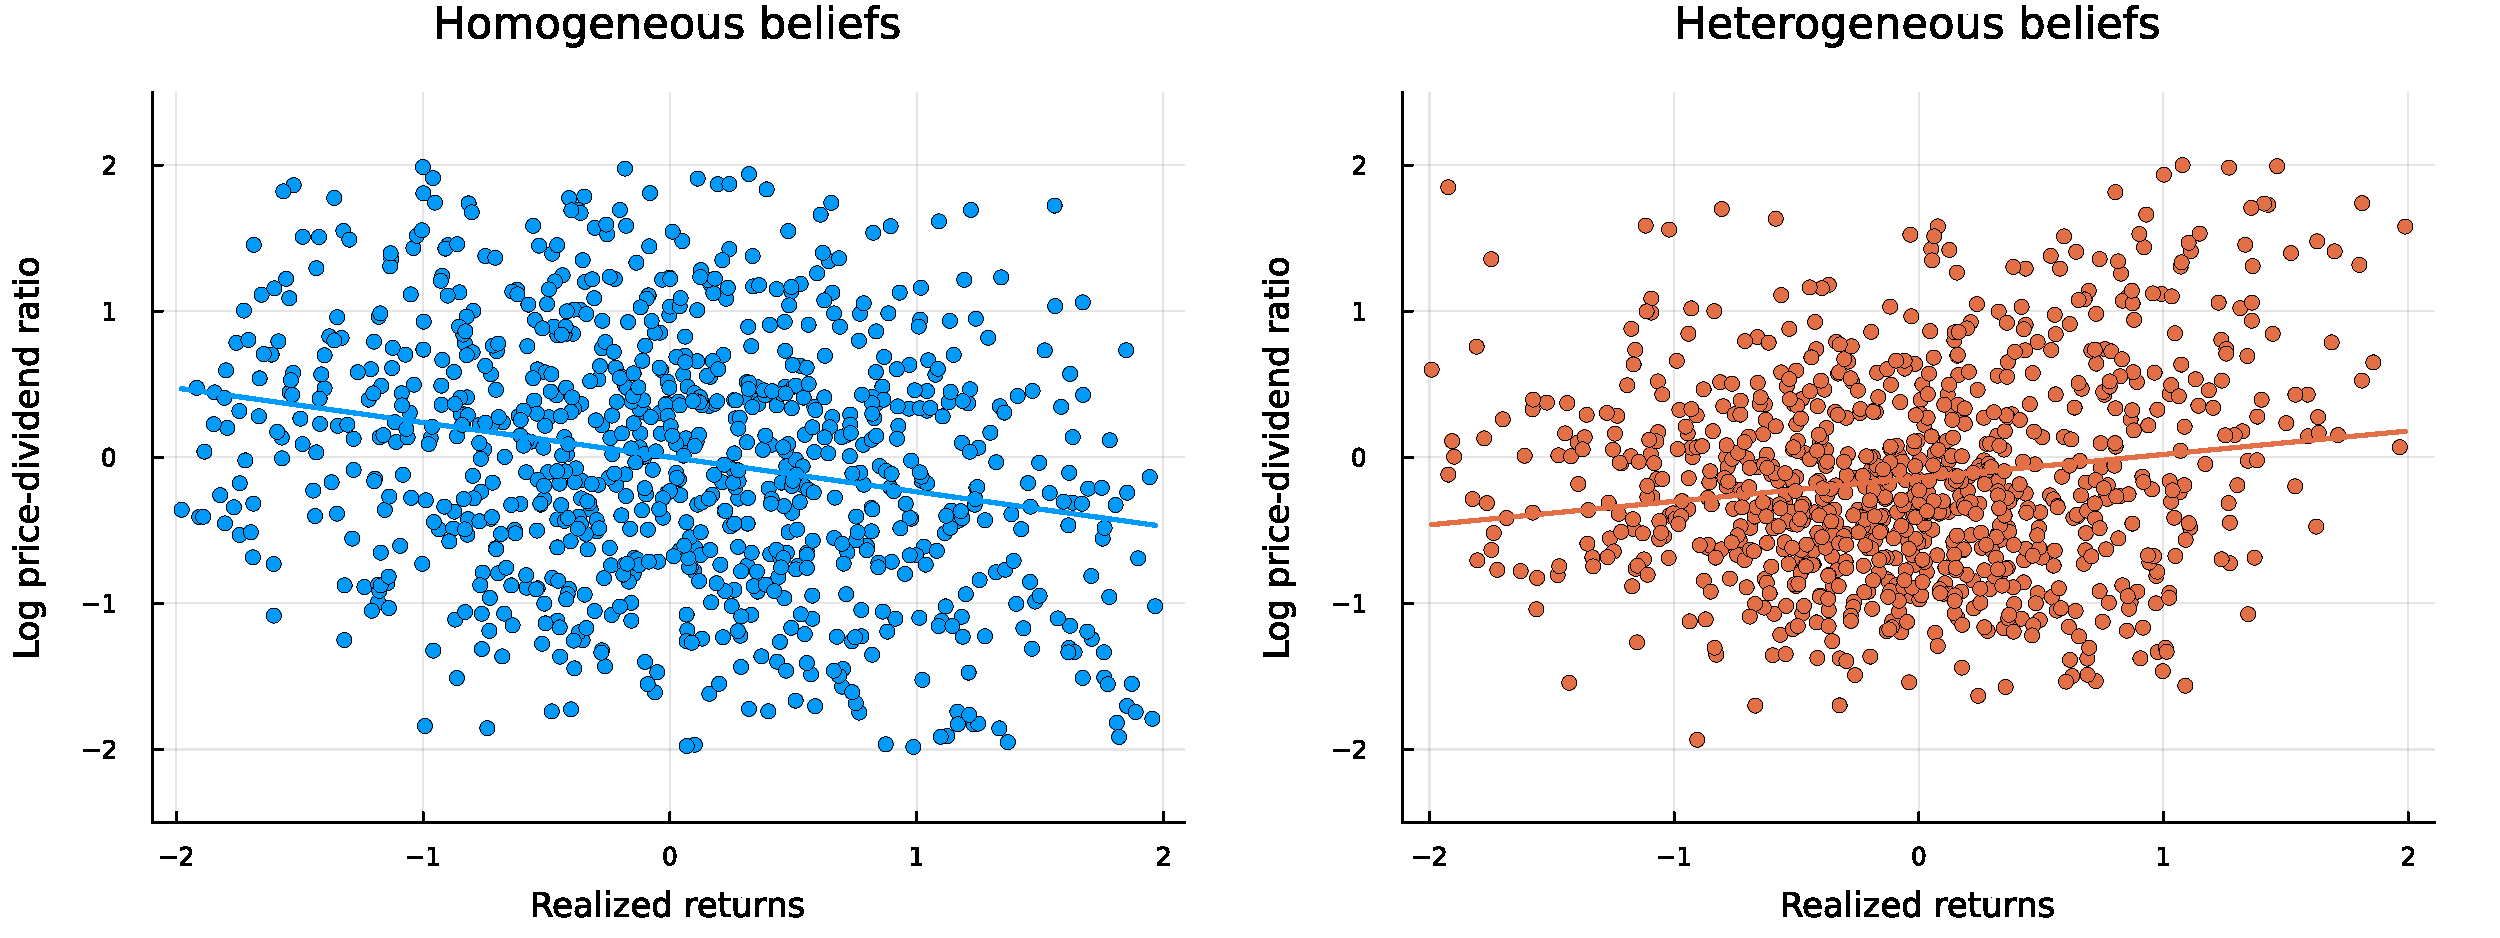
\includegraphics[width=0.99
            \textwidth]{figures/scatter_belief_comparison.pdf}
    \caption{Price amplification: homogeneous vs. heterogeneous beliefs}
    \caption*{  \scriptsize 
    Note: Figure shows a scatterplot of the log price-dividends and realized log returns in a 1,000-period simulation of the model. 
    The left panel shows the simulation for the model with homogeneous beliefs, and the right panel shows the simulation for the model with heterogeneous beliefs. 
    We standardized both variables and removed outliers to improve the visualization.\par} 
    \vspace{0.0cm}
    \label{fig: returns_pd_scatter}
\end{figure}

\q{QuantCol4}{Column 4 introduces heterogeneity in beliefs. 
It brings along rational investors and investors with distorted beliefs. 
The model now generates the level and volatility of asset prices consistent with the evidence, with significant volatility in hours.
To obtain a high equity premium, it is crucial to generate excess volatility of returns. 
This requires the price-dividend ratio to have the right comovement with returns. 
Figure~\ref{fig: returns_pd_scatter} shows that this is the case for the model with heterogeneous beliefs, but not for the model with homogeneous beliefs. 
This success is explained by the time-varying movements in the relative wealth of investors.}

\q{LaborSupplyElasticity}{Column 5 considers an alternative calibration with a higher labor supply elasticity, increasing it from 1.0 to 2.0, the upper limit of the estimates of the macro labor supply elasticity in \citet{keane2012micro}. 
Increasing the labor supply elasticity is motivated by the presence of unmodeled frictions: it is akin to increasing the real wage rigidities. 
While asset-price figures do not change substantially, the volatility of hours almost doubles, aligning the volatility of hours with that of the data.} 

Overall, aside from a modest overprediction of risk-free-rate volatility, the model with heterogeneous beliefs matches key asset-pricing and business-cycle moments.

\q{SV_Extension}{
    \paragraph{Extension with stochastic volatility.}
Appendix~\ref{app:sv_extension} extends the model to allow for stochastic volatility, following \citet{bansal2004risks}. Introducing volatility shocks modestly increases the equity premium and return volatility, while leaving macroeconomic moments largely unchanged. The qualitative conclusions of Table~\ref{tab:uncond_moments} remain intact.
}

\subsection{Excess volatility and return predictability}\label{sec:excess_volatility.sec}

The model's version with heterogeneous beliefs successfully generates empirically relevant levels of excess volatility, i.e., returns that are more volatile than cash flows.
Following \citet{cochrane1992explaining}, we can use a Campbell-Shiller approximation to decompose the variance of the price-dividend ratio into a cash-flow and a discount-rate component:
\begin{equation}\label{eq:var_decomposition}
    Var[pd_t] = Cov\left[ \sum_{k=1}^\infty \rho^k \Delta d_{t+k}, pd_t \right] - Cov\left[ \sum_{k=1}^\infty \rho^k r_{t+k}, pd_t \right],
\end{equation}
where $pd_t$ is the log price-dividend ratio, $\Delta d_{t+1}$ denotes log dividend growth, and $r_{t+1}$ denotes realized log returns.
Expression~\eqref{eq:var_decomposition} connects volatility and predictability. 
It shows that movements in the price-dividend ratio either predict changes in dividend growth or future returns. 
To quantify the relative importance of movements in discount rates, consider the share of variance explained by movements in expected returns, defined as $\beta_{r} \equiv -\frac{Cov\left[ \sum_{k=1}^\infty \rho^k r_{t+k}, pd_t \right]}{Var[pd_t]}$.
As shown, e.g., in \citet{cochrane2011presidential}, empirical evidence suggests that $\beta_{r} \approx 1$, so
discount rates explain most of the price-dividend ratio variance. 

\begin{table}[t!]
    \begin{minipage}[t!]{\textwidth}
      \begin{minipage}[b]{0.5\textwidth}
        \centering 
            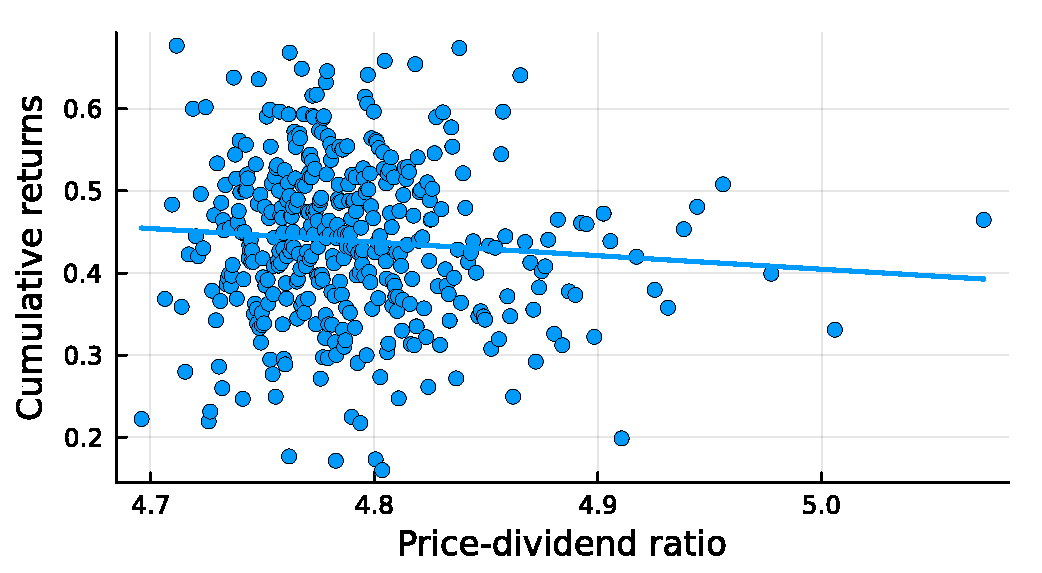
\includegraphics[width=0.99\textwidth]{figures/pd_forecast_binscatter.pdf}
        \captionof{figure}{Return predictability}\label{fig:pd_scatter}
        \end{minipage}
        \hfill
      \begin{minipage}[b]{0.5\textwidth}
        \centering
            \scriptsize
    \begingroup
    \centering\scalebox{0.99}{
    \begin{tabular}{lcccc}
       \tabularnewline \midrule \midrule
       Dependent Variable: & \multicolumn{4}{c}{cum\_ex\_returns}\\
       Model:         & (1)           & (2)            & (3)            & (4)\\  
       \midrule
       \emph{Variables}\\
       labor\_income    &   -2.07   &           & 0.33      &           \\   
                        &   (0.94)  &           & (1.31)    &           \\
       p/d              &           & -0.29     &           & -0.04     \\   
                        &           & (0.12)    &           & (0.17)    \\   
       \midrule
       Observations   & 4,000           & 4,000            & 4,000            & 4,000\\  
       \midrule \midrule
       %\multicolumn{5}{l}{\emph{Heteroskedasticity-robust standard-errors in parentheses}}\\
       \multicolumn{5}{l}{\emph{\textcolor{white}{Signif. Codes: ***: 0.01, **: 0.05, *: 0.1}}}\\
    \end{tabular}}
    \par\endgroup
          \captionof{table}{Labor and p/d ratio regressions}\label{table:pred_regression}
      \end{minipage}
      
      \end{minipage}    
          \caption*{\scriptsize 
        Note: The left panel shows a binscatter plot based on model simulations of the price-dividend ratio and a measure of future cumulative returns, $\sum_{k=1}^T \rho^{k-1} r_{t+k}$, for $T = 60$ quarters. We sort the first 4,000 observations by the price-dividend ratio into 400 equal-count bins and plot bin averages. The right panel shows the regression coefficients of future cumulative excess returns for $T = 60$ on the price-dividend ratio and labor income. 
        The data for the first two columns was simulated under the objective measure, while the data for the last two columns was simulated under subjective beliefs. Entries report Monte Carlo mean coefficients, and parentheses report the standard deviation across simulations.
         }
    \end{table}


    Given that $\beta_r$ corresponds to the slope of a regression of cumulative returns on the price-dividend ratio, the importance of discount rates to explain return volatility is tightly connected to the ability of the price-dividend ratio in predicting future long-run returns. 
    Figure~\ref{fig:pd_scatter} shows that the model with heterogeneous beliefs can capture the predictability patterns observed in the data. 
    The figure shows a strong negative association between the price-dividend ratio and cumulative returns in model-simulated data. 
    Moreover, the coefficient $\beta_r$ in models (4) and (5), as defined in Table~\ref{tab:uncond_moments}, is given by $\beta_r = 0.86$ and $\beta_r = 0.89$, respectively.
    In contrast, we have $\beta_r = -0.15$ for model (2), so the price-dividend ratio predicts returns with the wrong sign, and $\beta_r = 0.26$ for model (3), which has the correct sign but movements in cash flows drive the majority of the fluctuations in the price-dividend ratio. 
    Hence, only versions of the model with belief heterogeneity generate a degree of return predictability that aligns with the data.

    \paragraph{Labor income and return predictability.} 
    \q{OperationalLeverageQuant}{
    Time variation in risk premia generates fluctuations in hours worked in our setting. 
    As a result, in addition to the price-dividend ratio, movements in labor income should also predict excess returns.
    Table~\ref{table:pred_regression} reports the results of a regression of cumulative excess returns on the price-dividend ratio and labor income in our simulated data.
    Column 1 shows that periods of high labor income are associated with lower future returns.
    This finding is consistent with the evidence from \citet{santos2006labor}, who show that a high labor income share predicts lower aggregate stock returns.
    Similarly, \citet{belo2023drives} document that the aggregate hiring rate of publicly traded firms negatively predicts stock market excess returns.\footnote{
        \citet{belo2014labor} and \citet{favilukis2016does} show similar patterns for the cross-section of stock returns and U.S. states.
        For recent evidence using administrative data, see \citet{meeuwis2024time}.
    }    
    Our model links this evidence to fluctuations in subjective beliefs. 
    As discussed in Section~\ref{sec:analysis.sec4}, waves of optimism lead to both an increase in labor income and a compression of risk premia, jointly generating predictability from labor income and the price-dividend ratio. 
    }

    \paragraph{Subjective vs. objective predictability.} 
    The predictability results above are from the perspective of an econometrician. 
    Recent work by \citet{nagel2023dynamics} shows that return predictability looks very different under subjective beliefs: the standard predictors of returns are only weakly associated with survey-based measures of subjective risk premia. 
    While expected excess returns are countercyclical under the objective measure, they appear acyclical under subjective beliefs.
    
    Table~\ref{table:pred_regression} shows that the model replicates these empirical patterns.
    Columns 1 and 2 report predictability regressions using labor income and the price-dividend ratio as predictors under the objective measure. 
    In contrast, Columns 3 and 4 present the same regressions when the model is simulated under subjective beliefs.
    Consistent with \citet{nagel2023dynamics}, standard predictors are only weakly associated with future returns under subjective beliefs. The coefficient on labor income has the wrong sign and is statistically insignificant, while the coefficient on the price-dividend ratio is near zero.
    Thus, our model generates subjective risk premia that are essentially acyclical, which aligns with survey evidence. 
    As discussed in Section~\ref{sec:analysis.sec4}, this acyclicity arises because subjective expectations of future cash flows closely track asset price movements, dampening fluctuations in perceived risk premia.

% \subsection{Return predictability and excess volatility}
% % \paragraph{Connection with classic asset pricing tests.}
% The main postulate of the paper is that differences in beliefs regarding firm earnings growth rates amplify business cycles by affecting firm valuations. Campbell-Shiller, \citep{CampbellShiller88}, offer the following decomposition of the price-dividend ratio:
% \begin{equation}
% pd_{t}=\kappa + \sum^{\infty}_{\tau=0} \rho^{\tau} \mathbb{E}_{t}^{m}[g_{t+\tau}-r_{t+\tau}],
% \end{equation}
% where $pd_{t}$ stands for the log price dividend ratio, $g_{t}$ the growth of dividends and $r_{t+\tau}$ a subjective discount factor. Critically, $\mathbb{E}_{t}^{m}$ is the expectation of the representative market participant. This decomposition is the cornerstone of empirical asset pricing. 

% Because market expectations $\mathbb{E}_{t}^{m}$ are unobservable, we approximate expectations $\mathbb{E}_{t}^{s}[g_{t+\tau}]$ where $\mathbb{E}_{t}^{s}$ is a statistical expectation constructed from econometric models. A challenge put forth by \citet{CochraneDog} is that since aggregate dividends are difficult to forecast with price dividend ratios, the bulk of the movement in stock values must be attributed to changes in discounting. At face value, this conclusion would seem to leave little room for earnings beliefs driving asset prices. However, using $\mathbb{E}_{t}^{s}$ to proxy for $\mathbb{E}_{t}^{m}$, assumes rational expectations. 

% We can recast the Campbell-Shiller decomposition in terms of $\mathbb{E}_{t}^{s}$, $\mathbb{E}_{t}^{i}$ and $\mathbb{E}_{t}^{m}$ to decompose beliefs into deviations from rational expectations and the representativeness of survey data. 
% \begin{align}
% pd_{t}&=\kappa + 
% \overbrace{\sum^{\infty}_{\tau=0} \rho^{\tau} \left[ \mathbb{E}_{t}^{m}[g_{t+\tau}]-\mathbb{E}_{t}^{i}[g_{t+\tau}] \right]}^{\hbox{survey representativeness}}
% +\overbrace{\sum^{\infty}_{\tau=0} \rho^{\tau} \left[\mathbb{E}_{t}^{i}[g_{t+\tau}]-\mathbb{E}_{t}^{s}[g_{t+\tau}]\right]}^{\hbox{belief errors}}
% \\* &+\overbrace{
% \sum^{\infty}_{\tau=0} \rho^{\tau} \left[ \mathbb{E}_{t}^{s}[g_{t+\tau}]
% - \mathbb{E}_{t}^{m}[r_{t+\tau}]\right]}^{\hbox{rational expectations}},
% \end{align}
% Under rational expectations, $\mathbb{E}_{t}^{m}=\mathbb{E}_{t}^{s}$, in which case beliefs do not impact substantially asset prices.
% If beliefs are irrational, $\mathbb{E}_{t}^{m}\not=\mathbb{E}_{t}^{s}$, leaving room for a substantial contribution of beliefs in the volatility of asset prices.  In particular, this contribution will be captured by forecast errors. Let's use this decomposition to see what ingredients of our model are consistent with this classic decomposition.

% \begin{comment}
% \paragraph{Campbell-Shiller Decomposition.}

% The Campbell-Shiller decomposition expresses the log price-dividend ratio as a function of expected future dividend growth and discount rates:
% \begin{equation}
%     p_t - d_t = const. + \sum_{k=1}^T \rho^{k-1} \left[ \Delta d_{t+k}  - r_{t+k}\right] + \rho^T (p_{T} -d_T),
% \end{equation}
% where $\rho$ is a linearization constant. Taking the covariance of this expression with itself, following \citet{cochrane1992}, we obtain:
% \begin{equation}
%     var(p_t - d_t) = cov\left(\sum_{k=1}^T \rho^{k-1} d_{t+k}, p_{t} - d_t \right) - 
%      cov\left(\sum_{k=1}^T \rho^{k-1} r_{t+k}, p_{t} - d_t \right) +\rho^T cov(p_T-d_T,p_t-d_t).\nonumber
% \end{equation}
% \end{comment}

% A variance decomposition of the formula above leads to:
% \begin{equation}
%     1 = \frac{cov\left(\sum_{k=1}^T \rho^{k-1} d_{t+k}, pd_t \right)}{var(pd_t)}
%     -\frac{cov\left(\sum_{k=1}^T \rho^{k-1} r_{t+k}, pd_t \right)}{var(pd_t)} 
%     + \rho^T \frac{cov(pd_T,pd_t)}{var(pd_t)},\nonumber
% \end{equation}
% for large $T$. This equation highlights three possible explanations for variations in the price-dividend ratio: (i) it predicts future dividend growth, (ii) it predicts future returns, or (iii) there exists a rational bubble.

% Empirical evidence, as noted by \citet{cochrane2011presidential}, suggests that the second term is nearly one, meaning that the price-dividend ratio exhibits little predictive power for future dividends, while there is no strong evidence of a rational bubble. This pattern indicates that most of the variation in the price-dividend ratio is driven by fluctuations in discount rates rather than changes in expected future dividends.

% Our model is consistent with this empirical pattern. It generates limited predictability of future cash flows while ensuring that the bulk of price-dividend fluctuations are driven by discount rates. Defining $\omega_{ret}$ as:
% \begin{equation}
%     \omega_{ret} = -\frac{cov\left(\sum_{k=1}^T \rho^{k-1} r_{t+k}, pd_t \right)}{var(pd_t)}
% \end{equation}
% and setting $T = 15 \times 4$ (corresponding to 15 years), we find that $\omega_{ret}$ is approximately one in the data. 

% % \begin{table}[t!]
% % \begin{minipage}[t!]{\textwidth}
% %   \begin{minipage}[b]{0.5\textwidth}
% %     \centering 
% %     	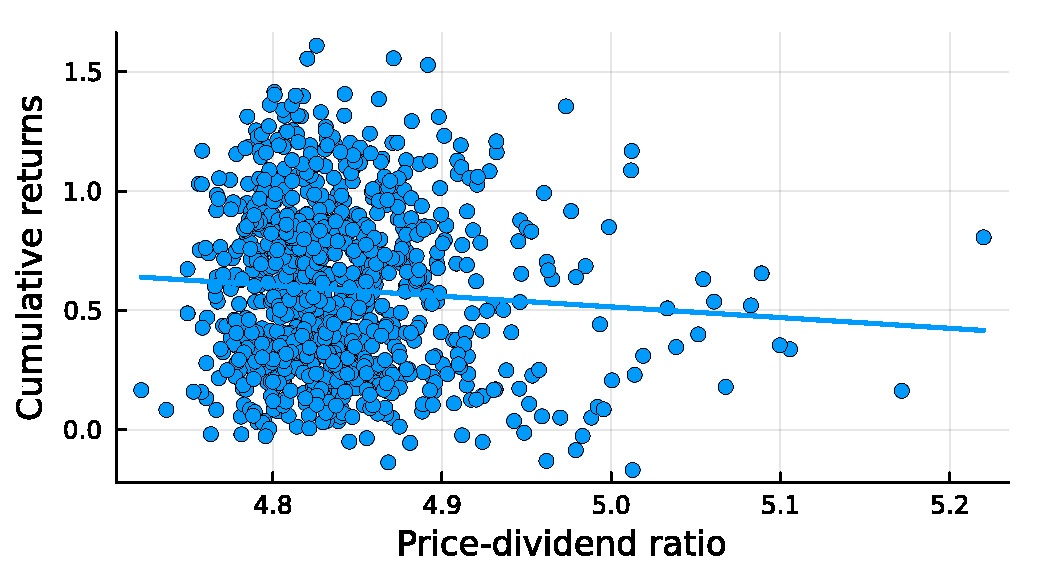
\includegraphics[scale=0.45]{figures/pd_forecast.pdf}
% %     \captionof{figure}{Return predictability}\label{fig:pd_scatter}
% %     \end{minipage}
% %     \hfill
% %   \begin{minipage}[b]{0.5\textwidth}
% %     \centering
% %     	\scriptsize
% % \begingroup
% % \centering\scalebox{0.9}{
% % \begin{tabular}{lcccc}
% %    \tabularnewline \midrule \midrule
% %    Dependent Variable: & \multicolumn{4}{c}{cum\_returns}\\
% %    Model:         & (1)           & (2)            & (3)            & (4)\\  
% %    \midrule
% %    \emph{Variables}\\
% %    p/d    & -0.91       &  & -0.95        & \\   
% %                   & (0.04)      &        & (0.04)       & \\   
% %    labor\_income           &  &   -0.71             & & -0.72\\   
% %                   &      &   (0.19)             &   & (0.20)\\
% %    \midrule
% %    \emph{Fit statistics}\\
% %    Observations   & 4,000           & 4,000            & 4,000            & 4,000\\  
% %    R$^2$          & 0.138       & 0.003        & 0.131        & 0.003\\   
% %    \midrule \midrule
% %    %\multicolumn{5}{l}{\emph{Heteroskedasticity-robust standard-errors in parentheses}}\\
% %    \multicolumn{5}{l}{\emph{\textcolor{white}{Signif. Codes: ***: 0.01, **: 0.05, *: 0.1}}}\\
% % \end{tabular}}
% % \par\endgroup
% %       \captionof{table}{Labor and p/d ratio regressions}\label{table:pred_regression}
% %   \end{minipage}
  
% %   \end{minipage}    
% %   	\caption*{\scriptsize 
% % 	Note: The left panel shows a scatter plot based on model simulations of the price-dividend ratio and a measure of cumulative future returns, $\sum_{k=1}^T \rho^{k-1} r_{t+k}$, for $T = 60$ quarters. The right panel shows the regression coefficients of future cumulative returns for $T = 60$ (first two columns) and $T = 120$ (last two columns) on the price-dividend ratio and labor income. }
% % \end{table}

% This outcome is not mechanical, in the scenario of column (1) where the price-dividend ratio does not vary, $\omega_{ret}$ is undefined. Introducing non-rational beliefs, in column (3), we obtain $\omega_{ret} = -0.16$, which suggests that the model initially dampens return volatility instead of amplifying it, moving in the wrong direction relative to empirical observations. Allowing for richer belief heterogeneity improves the fit, yielding $\omega_{ret} = 0.40$, meaning predictability shifts in the correct direction but still places too much volatility on the cash-flow channel. With further refinements, our preferred specifications reach $\omega_{ret} = 0.93$ and $\omega_{ret} = 0.97$, successfully capturing the empirical finding that most fluctuations in the price-dividend ratio stem from changes in discount rates rather than in expected dividends.
% % , even though the data generating process includes non-rational behavior. 
% This can be seen in Figure~\ref{fig:pd_scatter}, which shows a scatter plot of the price-dividend ratio and future expected returns, as measured by $\sum_{k=1}^T \rho^{k-1} r_{t+k}$. 
% The figure shows how the model with subjective beliefs leads to time-variation in expected returns from the point of view of an econometrician. 


% Importantly, our model avoids the critique raised by \citet{beeler2012long}. 
% Long-run risk models typically predict that the price-dividend ratio should forecast future consumption and dividend growth, a pattern not supported by the data. In contrast, our model does not rely on this channel, sidestepping this issue. Furthermore, our framework aligns well with recent empirical findings by \citet{nagel2023dynamics}, which document that objective discount rates are more cyclical than subjective ones. The model also captures the empirical relationship identified by \citet{santos2006labor}, who provide evidence that labor income predicts future returns.
% Table~\ref{table:pred_regression} shows the result of regressions in simulated data of future cumulative returns on the price-dividend and also labor income. 
% We can see that periods of high labor income predict low future returns, consistent with the connection between labor income and risk premia discussed in Section~\ref{sec:analysis.sec4}. 

% The mechanism underlying these results is straightforward: The model introduces belief heterogeneity, leading to fluctuations in risk premia that impact firm hiring and investment decisions. These movements in discount rates, rather than cash flows, drive asset price fluctuations, aligning our model with the dominant explanation observed in the data. This connection between labor markets, asset prices, and belief heterogeneity provides a unified framework for understanding business cycles and financial markets.












\begin{comment}
\paragraph{Discussion: Beliefs and the Operating Leverage Channel.}

We also know that the labor share would be constant if labor were chosen after productivity was known. Thus, operating leverage, defined as the ratio of revenues minus contemporary variable costs---zero in our setting---to profits would be constant. Yet, there is evidence of xxx correlation, see, e.g., \citet{novy2010operating} and \citet{donangelo2019cross}.\footnote{The relationship between return risk and operating leverage initially appears in \citet{lev1974association}.}. In turn, TFP shocks disproportionately impact dividends relative to consumption; a pattern of more volatile dividends than consumption is consistent with the data  (see, e.g., \citealt{campbell2003consumption}) but inconsistent with models in which hiring is not risky.

%\footnote{This channel is analogous to how changes in the cost of capital, the sum of the interest rate and the firm's risk premium, affects investment decisions.
%The key difference is that the costs and benefits of hiring an additional worker are incurred at the same time, so it is the risk premium, instead of the cost of capital, that affects the hiring decision.
%}
\end{comment}

 


\section{Conclusion}\label{sec:conclusion}
% When asked about the nature of business cycles, Thomas Sargent\footnote{Hyman Minsky was Thomas Sargent's undergraduate advisor. Whereas Sargent departs methodologically and calls for a quantitative approach to economic research, there is an agreement in their views regarding nature of business cycles.}, a rational expectations pioneer, answered:\footnote{Interview with Thomas Sargent, \emph{The Region}, August 26, 2010. Available at https://www.minneapolisfed.org/article/2010/interview-with-thomas-sargent.}  
% \begin{quote}
% ``[...] economists have been working hard to refine rational expectations theory. [...] An influential example of such work is the 1978 QJE paper by Harrison and Kreps. [...], for policymakers to know whether and how they can moderate bubbles, we need to have well-confirmed quantitative versions of such models up and running."
% \end{quote} 
% This response embraces the idea that ``belief heterogeneity" matters but also calls for quantitative models that link beliefs with the real economy. 

% This paper responds to that call and adapts a standard real business cycle and asset pricing model to fit the narrative that waves of optimism and pessimism drive the business cycle. We argue that a combination of heterogeneity in beliefs, with substantial extrapolation, coupled with an operating leverage channel, can successfully reproduce business cycle, asset pricing and survey data patterns. Extrapolative beliefs and heterogeneity deliver the amplification that is key for this success. Extrapolation adds to risk build up. 

% We foresee that our framework can be extended to study the interaction with other forms of amplification. 
%         Namely, nominal rigidities open the door to amplification through aggregate demand externalities. 
%         Additional financial frictions, such as margin calls or short-selling constraints, can amplify asset prices through fire-sale and pecuniary externalities that impact wealth and risk-taking capacity. 
%         We expect our conclusions to remain relevant in contexts with these additional frictions.


\q{Conclusion}{When asked about the nature of business cycles, Thomas Sargent emphasized that
progress requires quantitative models that discipline deviations from rational
expectations and confront them with the data:\footnote{Interview with Thomas Sargent, \emph{The Region}, August 26, 2010.}
\begin{quote}
"[...] economists have been working hard to refine rational expectations theory. [...] An influential example of such work is the 1978 QJE paper by Harrison and Kreps. [...], for policymakers to know whether and how they can moderate bubbles, we need to have well-confirmed quantitative versions of such models up and running."
\end{quote}

This paper responds to that call. We develop a tractable macro-finance framework
in which heterogeneous and extrapolative beliefs interact with production and labor
demand to generate endogenous movements in risk premia, asset prices, and real
activity.

Quantitatively, the model matches a wide range of empirical patterns in survey expectations,
trading volume, return predictability, and business-cycle dynamics. These results
arise from the interaction between belief dispersion, wealth dynamics, and operating
leverage.

Although our benchmark specification is deliberately parsimonious, with a simple
productivity process and two investor types, the framework is substantially more
general. The Markov structure accommodates richer technology dynamics, stochastic
volatility, alternative belief processes, and additional investor types or frictions.
The simplicity of the baseline clarifies the mechanism; it does not limit the model's
scope.

Our framework provides a disciplined way to embed waves of optimism and pessimism
into a standard macroeconomic environment while remaining flexible enough to
incorporate additional amplification mechanisms. We view this as a step toward
quantitatively credible models in which confidence fluctuations are measurable
forces with testable implications.}

\singlespace
\bibliography{../utils/references/references,../utils/references/references_empirical}


\newpage
\appendix
\part*{Online Appendix}\label{appendix}
\numberwithin{equation}{section}
\setcounter{page}{1}
\onehalfspace
\section{Proofs}\label{app: proofs}

\subsection{Derivation of the investor's modified problem}\label{app: proof_investor_problem}

We start by providing a derivation of the investor's modified problem. 
\begin{proof}
    First, we adopt a change of variables and write the investor's problem as follows
    \begin{equation}\label{eq: app_investor_problem}
        V_{i,t} = \max_{\{\tilde{C}_{i,t}, h_{i,t}, B_{i,t}, S_{i,t}\}} (1-\beta) U\left(\tilde{C}_{i,t} \right) + \beta U\left( \Psi^ {-1}\left( \mathbb{E}_{i,t}\left[ \Psi\left( U^ {-1}(V_{i,t+1}\right)\right] \right)  \right),
    \end{equation}
    subject to 
    \begin{equation}\label{eq: app_flow}
            \tilde{C}_{i,t} + Q_t S_{i,t} + B_{i,t} = R_{e,t} Q_{t-1} S_{i,t-1} + R_{b,t} B_{i,t-1} + W_t h_{i,t} -\xi_t \frac{h_{i,t}^{1+\nu}}{1+\nu},
    \end{equation}
    and the natural borrowing
    \begin{equation}\label{eq: app_natural_limit}
        (Q_t+\pi_t) S_{i,t-1} + R_{b,t} B_{i,t-1} + W_t h_{i,t} -\xi_t \frac{h_{i,t}^{1+\nu}}{1+\nu} \geq -\mathcal{H}_{i,t}
    \end{equation}
    It is immediate that the optimal value of $h_{i,t}$ satisfies
    \begin{equation}\label{eq: app_optimal_h}
        W_t = \xi_t h_{i,t}^\nu.
    \end{equation}
    
    We show next that, given $h_{i,t}$ satisfying \eqref{eq: app_optimal_h}, if the sequence $(\tilde{C}_{i,t},B_{i,t}, S_{i,t})$ satisfies \eqref{eq: app_flow} and \eqref{eq: app_natural_limit}, then     there exists $(N_{i,t}, \omega_{i,t})$ such that $(\tilde{C}_{i,t}, N_{i,t}, \omega_{i,t}) $ satisfies \eqref{eq:lom_N} and $N_{i,t} \geq 0$. 
    Conversely, if $(\tilde{C}_{i,t}, N_{i,t}, \omega_{i,t}) $ satisfies \eqref{eq:lom_N} and $N_{i,t} \geq 0$, there exists $(B_{i,t}, S_{i,t})$ such that  $(\tilde{C}_{i,t},B_{i,t}, S_{i,t})$         satisfies \eqref{eq: app_flow} and \eqref{eq: app_natural_limit}.
    
    From the definition of the return on human wealth, we have that $W_t h_{i,t} -\xi_t \frac{h_{i,t}^{1+\nu}}{1+\nu} = R_{h,t-1} \mathcal{H}_{i,t-1} - \mathcal{H}_{i,t}$, which allow us to write \eqref{eq: app_flow} and \eqref{eq: app_natural_limit} as follows:
    \begin{equation}\label{eq: app_flow_N}
        \tilde{C}_{i,t} + Q_t S_{i,t} + B_{i,t} + \mathcal{H}_{i,t} = N_{i,t}, \qquad \qquad N_{i,t} \geq 0.
    \end{equation}
    
    % As hours are equalized across investors, then the return on human wealth is same for all investors, allowing us to write $R_{h_i,t} = R_{h,t}$.
    We consider next the law of motion of total wealth:\small
    \begin{align}
        N_{i,t+1} =\left[ R_{e,t+1} \frac{Q_{t} S_{i,t}}{Q_{t} S_{i,t}+B_{i,t}+\mathcal{H}_{i,t}} + R_{b,t+1} \frac{B_{i,t}}{Q_{t} S_{i,t}+B_{i,t}+\mathcal{H}_{i,t}}+ R_{h_i,t+1} \frac{\mathcal{H}_{i,t}}{Q_{t} S_{i,t}+B_{i,t}+\mathcal{H}_{i,t}}\right] \left( N_{i,t} -\tilde{C}_{i,t}\right).
    \end{align}\normalsize
    
    As markets are dynamically complete, there exists replicating portfolios $(\omega_{h_i,t}, \omega_{e,t})$ such that 
    \begin{equation}
        R_{k,t+1} = \omega_{k,t} R_{r,t+1} + (1-\omega_{k,t}) R_{b,t+1},
    \end{equation}
    for $k\in\{h_i,e\}$.
    
    Combining the previous two conditions, we obtain\small
    \begin{align}
        N_{i,t+1} =\left[ R_{r,t+1} \frac{\omega_{e,t} Q_{t} S_{i,t}+\omega_{h_i,t} \mathcal{H}_{i,t}}{N_{i,t}-\tilde{C}_{i,t}} + R_{b,t+1} \frac{B_{i,t}+(1-\omega_{e,t}) Q_t S_{i,t}+(1-\omega_{h_i,t}) \mathcal{H}_{i,t}}{N_{i,t}-\tilde{C}_{i,t}}\right] \left( N_{i,t} -\tilde{C}_{i,t}\right).
    \end{align}\normalsize
    
    Using the first condition in \eqref{eq: app_flow_N} to solve for $B_{i,t}$, we obtain
    \begin{equation}
        N_{i,t+1} =\left[ \left(R_{r,t+1} - R_{b,t+1}\right) \omega_{i,t} + R_{b,t+1} \right] \left( N_{i,t} -\tilde{C}_{i,t}\right),
    \end{equation}
    where $\omega_{i,t} \equiv \frac{\omega_{e,t} Q_{t} S_{i,t}+\omega_{h_i,t} \mathcal{H}_{i,t}}{N_{i,t}-\tilde{C}_{i,t}}$.
    
    
    
    \end{proof}

\subsection{Proof of Lemma~\ref{lemma: policy_functions}} \label{app: proof_policy_functions}

The next lemma characterizes the value function, the consumption function, and the Euler equations of each investor.

\begin{lemma}[Consumption and Euler equations]\label{lemma: policy_functions}
The household's value function takes the form: 
$V_{i}(N,X,s)=U\left(v_{i}(X,s)N\right),$
where $v_{i}(X,s)$ denotes the \textit{wealth multiplier}. The consumption-wealth
ratio $c_{i}(X,s)=\frac{\tilde{C}_{i}(N,X,s)}{N}$ and Euler equations
for investor $i\in\mathcal{I}$ are given by
\begin{enumerate}[(i)]
\item Consumption-wealth ratio:
\begin{equation}
c_{i}(X,s)=\frac{(\beta^{-1}-1)^{\psi}\mathcal{R}_{i}(X,s)^{1-\psi}}{1+(\beta^{-1}-1)^{\psi}\mathcal{R}_{i}(X,s)^{1-\psi}},\label{eq: c_n}
\end{equation}
where $\mathcal{R}_{i}(X,s)\equiv\Psi^{-1}\left(\mathbb{E}_{i}\left[\Psi\left(v(X',s')R_{i}(X,s,s')\right)|X\right]\right)$.
\item Euler equation for an asset $j\in\{r,b\}$: 
\begin{equation}
1=\mathbb{E}_{i}\left[\left.\Lambda_{i}(X,s,s')R_{j}(X,s,s')\right.\right],\label{eq: eulers_app}
\end{equation}
where, for $\theta\equiv\frac{1-\gamma}{1-\psi^{-1}}$, the investor's SDF is given by 
\begin{equation}
\Lambda_{i}(X,s,s')=\beta^{\theta}\left(\frac{c_{i}(\chi(X,s,s'),s')N'}{c_{i}(X,s)N}\right)^{-\frac{\theta}{\psi}}R_{i}(X,s,s')^{-(1-\theta)}.
\end{equation}
\item The wealth multipliers satisfy:
\begin{equation}
v_{i}(X,s)=U^{-1}\left[U\left(c_{i}(X,s)\right)+\beta U\left(\mathcal{R}_{i}(X,s)\left(1-c_{i}(X,s)\right)\right)\right].\label{eq:value.recursion}
\end{equation}
\end{enumerate}
\end{lemma}
% The value function here equals the static utility evaluated at $v_{i}(X,s)N$.\footnote{
%     The wealth multiplier $v_{i}(X,s)$ is a measure of welfare: $v_{i}(X,s)N$ corresponds to the constant consumption level that achieves the investor's expected utility. 
%     This term is analogous to \cite{lucas1987models} measure of the welfare cost of business cycles.}
%     % ---the constant level of consumption that achieves the same utility as in the original stochastic economy.} 
% The consumption-wealth ratio in (\ref{eq: c_n})
% coincides with the consumption-wealth ratio of a deterministic problem
% with return $\mathcal{R}_{i}(X,s)$. In turn, $\mathcal{R}_{i}(X,s)$
% is a risk-adjusted portfolio return with states weighted by a multiplier,
% $v(X',s')$, that solves the recursion in Equation (\ref{eq:value.recursion}). The effect of $\mathcal{R}_{i}$ on consumption depends
% only on the EIS coefficient, $\psi$, that captures substitution and
% income effects. When $\psi=1$, income and substitution effects cancel
% out; the consumption-wealth ratio is $c_{i}(X,s)=1-\beta$. The following
% section derives several results under this parameterization.


\begin{proof}
First, we verify that the value function takes the form \eqref{eq: value_function}. Given the conjecture about the value function, the Bellman equation for investor $i$ can be written as
\begin{equation}
    \frac{(v_i(X,s) N)^{1-\psi^{-1}}-1}{1-\psi^{-1}} = \max_{\tilde{c}_{i},\omega_{i}}  (1-\beta) \frac{(\tilde{c}_i N)^{1-\psi^{-1}}-1}{1-\psi^{-1}} + \beta \frac{\mathbb{E}_i\left[ (v_i(X',s')N')^{1-\gamma}\right]^{\frac{1-\psi^{-1}}{1-\gamma}}-1}{1-\psi^{-1}},
\end{equation}
subject to $N' = R_{i}(X,s,s') (1-\tilde{c}_i) N$ and $N'\geq 0$.

The first-order conditions for the consumption-wealth ratio and the portfolio share are given by 
\begin{align}
    (1-\beta) \tilde{c}_i^{-\psi^{-1}} &= \beta \mathcal{R}_i(X,s)^{1-\psi^{-1}} (1-\tilde{c}_i)^{-\psi^{-1}}\\
    0& = \mathbb{E}_i\left[ (v_i(X',s') R_{i,n}(X,s,s'))^{-\gamma} v_i(X') (R_{r}(X,s,s') - R_b(X,s))  \right]
\end{align}
where $\mathcal{R}_i(X,s) = \mathbb{E}_i\left[ (v_i(X',s') R_{i}(X,s,s'))^{1-\gamma} |X,s\right]^{\frac{1}{1-\gamma}}$.

Given $\mathcal{R}_i(X,s)$, we can solve for the consumption-wealth ratio:
\begin{equation}
    \tilde{c}_i(X,s) = \frac{ (\beta^{-1}-1)^{\psi} \mathcal{R}_i(X,s)^{1-\psi}}{1+ (\beta^{-1}-1)^{\psi} \mathcal{R}_i(X,s)^{1-\psi}}.
\end{equation}

The envelope condition with respect to $N$ is given by
\begin{equation}\label{eq: app_envelope}
    v_i(X)^{1-1/\psi} = \beta \mathcal{R}_i(X) ^{1-1/\psi}  (1-\tilde{c}_i(X))^{-1/\psi} \Rightarrow 
    \tilde{c}_i(X) = (1-\beta)^{\psi} v_i(X)^{1-\psi}.
\end{equation}

From the optimality condition for the risky asset, we obtain 
\begin{equation}\label{eq: app_optimality_omega}
    \mathbb{E}_i\left[  (v_i(X',s') R_{i}(X,s,s'))^{1-\gamma}  \right] = \mathbb{E}_i\left[  v_i(X',s')^{1-\gamma} R_{i}(X,s,s')^{-\gamma} R_j(X,s,s') \right],
\end{equation}
for $j \in \{r,b\}$.

Raising the envelope condition \eqref{eq: app_envelope} to the power $\theta \equiv \frac{1-\gamma}{1-\psi^{-1}}$, using the definition of $\mathcal{R}_i(X)$ and condition \eqref{eq: app_optimality_omega}, we obtain
\begin{equation}
    1 = \mathbb{E}_i\left[ \beta^\theta \left(\frac{v_i(X',s')}{v_i(X,s')}\right)^{1-\gamma} R_{i}(X,s,s')^{-\gamma} R_j(X,s,s') (1-\tilde{c}_i(X,s))^{-\theta/\psi } \right].
\end{equation}

Using the condition $v_i(X) = (1-\beta)^{\frac{1}{1-\psi^{-1}}} \tilde{c}_i(X)^{-\frac{\psi^{-1}}{1-\psi^{-1}}}$, we obtain the Euler equations
\begin{equation}
    1 = \mathbb{E}_i\left[ \beta^\theta \left(\frac{\tilde{c}_i(X',s') N'}{\tilde{c}_i(X,s) N}\right)^{-\frac{\theta}{\psi}} R_{i}(X,s,s')^{-(1-\theta)} R_j(X,s,s') \right].
\end{equation}

This concludes the derivation of the consumption-wealth ratio and the Euler equations for the two assets. It remains to check that the value function takes the form \eqref{eq: value_function}, which amounts to show that $v_i(X)$ indeed does not depend on $N$. Notice that $\tilde{c}_i(X,s)$ and $\omega_i(X,s)$ do not depend on $N$. We can then write the Bellman equation as follows:
\begin{equation}
    v_i(X,s)^{1-\psi^{-1}} =  (1-\beta) \tilde{c}_i(X,s)^{1-\psi^{-1}} + \beta \mathbb{E}_i\left[ (v_i(X',s')R_{i}(X,s,s')(1-\tilde{c}_i(X)))^{1-\gamma}\right]^{\frac{1-\psi^{-1}}{1-\gamma}},
\end{equation}
for $\psi \neq 1$ and
\begin{equation}
    \log v_i(X,s) = (1-\beta) \log \tilde{c}_i(X,s) + \beta \log \mathbb{E}_i\left[ (v_i(X',s')R_{i}(X,s,s')(1-\tilde{c}_i(X,s)))^{1-\gamma}\right]^{\frac{1}{1-\gamma}}.
\end{equation}
which is independent of $N$, which confirms our conjecture for the value function \eqref{eq: value_function}.


\end{proof}


\subsection{Proof of Lemma \ref{lemma: portfolio_share}}\label{app: proof_portfolio_share}
    
The following lemma characterizes households' portfolio
weight in terms of the economy-wide SDF, the market
prices, and their beliefs.

\begin{lemma}[Portfolio share]\label{lemma: portfolio_share} The
shares of total wealth invested in the risky asset are 
\begin{equation}
\omega_{i}(X,s)=\frac{1}{\Delta R_{r}(X,s)}\left[\frac{\tilde{p}_{i}(X,s,H)}{p_{s,H}\Lambda(X,s,H)}-\frac{\tilde{p}_{i}(X,s,L)}{p_{s,L}\Lambda(X,s,L)}\right],\label{eq: portfolio_share}
\end{equation}
where $\tilde{p}_{i}(X,s,s')$ is 
\[
\tilde{p}_{i}(X,s,s')=\frac{(p_{ss'}^{i})^{\frac{1}{\gamma}}\left[v_{i}(\chi(X,s,s'),s')|R_{r}^{e}(X,s,s')|\right]^{\frac{1}{\gamma}-1}}{\sum_{\tilde{s}'\in\{L,H\}}(p_{s\tilde{s}'}^{i})^{\frac{1}{\gamma}}\left[v_{i}(\chi(X,s,\tilde{s}'),\tilde{s}')|R_{r}^{e}(X,s,\tilde{s}')|\right]^{\frac{1}{\gamma}-1}}.
\]
\end{lemma}
Lemma \ref{lemma: portfolio_share}, describes how portfolio shares
depend on distorted probabilities, $\tilde{p}_{i}(X,s,s')$, and
$p_{ss'}\times\Lambda(X,s,s')$. 
The portfolio share $\omega_{i}(X,s)$ in (\ref{eq: portfolio_share}) is increasing in $p_{sH}^{i}$. 
This means that relatively optimistic investors hold more of the risky asset. 

\begin{proof}
Let $X' =\chi(X,s,s')$. 
The optimal portfolio share satisfies the condition
\begin{equation}
    \frac{p_{sL}^i}{p_{sH}^i} \frac{v_i(\chi(X,s,L), L)^{1-\gamma} }{v_i(\chi(X,s,H), H)^{1-\gamma} }\left( \frac{\omega_i(X,s) R_r^e(X,s,L) + 1  }{\omega_i(X,s) R_r^e(X,s,H) + 1  }\right)^{-\gamma}\frac{|R_r^e(X,s,L)|}{R_r^e(X,s,H)} = 1
\end{equation}

Raising both sides to $-\frac{1}{\gamma}$, we obtain
\begin{equation}
    \left(\frac{p_{sL}^i}{p_{sH}^i}\right)^{-\frac{1}{\gamma}} \frac{v_i(\chi(X,s,L), L)^{1-\frac{1}{\gamma}} }{v_i(\chi(X,s,H), H)^{1-\frac{1}{\gamma}} } \frac{\omega_i(X,s) R_r^e(X,s,L) + 1  }{\omega_i(X,s) R_r^e(X,s,H) + 1 }\frac{|R_r^e(X,s,L)|^{-\frac{1}{\gamma}}}{R_r^e(X,s,H)^{-\frac{1}{\gamma}}} = 1
\end{equation}

Rearranging the expression above, we obtain
\begin{equation}\label{app:omega_returns}
\omega_{i}(X,s) =  \frac{\tilde{p}_i(X,s,H)}{|R_r^e(X,s,L)|} -  \frac{\tilde{p}_i(X,s,L)}{R_r^e(X,s,H)}, 
\end{equation}
where
\begin{equation}
    \tilde{p}_{i}(X,s,s') = \frac{(p_{ss'}^i)^{\frac{1}{\gamma}} \left[ v_{i}(\chi(X,s,s'),s') |R_r^e(X,s,s')| \right]^{\frac{1}{\gamma}-1}}{\sum_{s'\in \{L,H\} } (p_{ss'}^i)^{\frac{1}{\gamma}} \left[ v_{i}(\chi(X,s,s'),s') |R_r^e(X,s,s')| \right]^{\frac{1}{\gamma}-1} }.
\end{equation}

The SDF in this economy is given by
\begin{align}
    \Lambda(X,s,s') &= \frac{1}{p_{ss'}} \frac{1}{R_f(X,s)} \frac{|R_r(X,s,-s')-R_f(X,s)|}{\Delta R_{r}(X,s)},
\end{align}
where $\Delta R_r(X,s) = R_r(X,s,H) - R_r(X,s,L)$.

We can then write $\omega_{i}(X,s)$  as follows
\begin{equation}
    \omega_i(X,s) = \frac{1}{\Delta R_r(X,s)} \left[\frac{\tilde{p}_i(X,s,H)}{p_{s,H} \Lambda(X,s,H)}  -\frac{\tilde{p}_i(X,s,L)}{p_{s,L}\Lambda(X,s,L)} \right].
\end{equation}

\paragraph{Log utility.} The formula above simplifies under the case of log utility. 
First, we obtain $\tilde{p}_i(X,s,s') = p_{ss'}^i$. This allows us to write the portfolio share as follows:
\begin{equation}
    \omega_i(X,s) = \frac{p_{s,H}^i}{|R_r^e(X,s,L)|}  -\frac{p_{s,L}^i}{R_r^e(X,s,H)},
\end{equation}
using the expression for $\Lambda(X,s,s')$ and the fact that $R_r^e(X,s,L) < 0 < R_r^e(X,s,H)$ under log utility.

We can rewrite the expression above as follows:
\begin{equation}
    \omega_i(X,s) = \frac{p_{s,H}^i R_r^e(X,s,H) + p_{s,L}^i R_r^e(X,s,L)}{|R_r^e(X,s,L)|R_r^e(X,s,H)} = \frac{\mathbb{E}_{i,s}[R_r^e(X,s,s')]}{|R_r^e(X,s,L)|R_r^e(X,s,H)}.
\end{equation}

The denominator in the expression above can be written as follows:
\begin{align}
    |R_r^e(X,s,L)|R_r^e(X,s,H) = \frac{\mathcal{L}'(X,s) - x_L}{(1-\alpha)\mathcal{L}'(X,s) } \frac{x_H - \mathcal{L}'(X,s)}{(1-\alpha)\mathcal{L}'(X,s) }.
\end{align}

The risk-neutral expectation of productivity growth can be written as follows:
\begin{equation}
    \mathcal{L}'(X,s) = p_{sH}^{RN}(X,s) x_H + p_{sL}^{RN}(X,s) x_L.
\end{equation}
where $p_{ss'}^{RN}(X,s)$ is the risk-neutral probability of state $s'$ given state $s$.

Combining the previous two expressions we obtain:
\begin{equation}
    |R_r^e(X,s,L)|R_r^e(X,s,H)= p_{sH}^{RN}(X,s) p_{sL}^{RN}(X,s) \Delta R_r^e(X,s)^2,
\end{equation}
where $\Delta R_r^e(X,s) = R_r^e(X,s,H) - R_r^e(X,s,L) = \frac{\Delta x}{(1-\alpha) \mathcal{L}'(X,s)} $. 
The expression above is the variance of the excess return on the risky asset under risk-neutral probabilities.

The risk-neutral probability of state $s'$ given state $s$ is given by
\begin{equation}
    p_{ss'}^{RN}(X,s) =\frac{p_{ss'} \Lambda(X,s,s')}{\mathbb{E}_s[\Lambda(X,s,s')]} = \frac{R_r^e(X,s,-s')}{\Delta R_r^e(X,s)}.
\end{equation}

We can then write the risk-neutral probabilities as follows:
\begin{equation}
    p_{sL}^{RN}(X,s) = \frac{R_r^e(X,s,H)}{\Delta R_r^e(X,s)} = \frac{x_H - \mathcal{L}'(X,s)}{\Delta x }, \qquad 
    p_{sH}^{RN}(X,s) = \frac{R_r^e(X,s,L)}{\Delta R_r^e(X,s)} = \frac{\mathcal{L}'(X,s)-x_L}{\Delta x }.
\end{equation}

\paragraph{Diffusion-like approximation.} To better interpret the expression for the portfolio share, it is useful to consider an approximation analogous to the continuous-time limit for diffusion processes. Given $R_{r}(X,s,s')$,  probabilities $p_{ss'}^i$ for household $i$, and a small parameter $\epsilon >0$, we can find $\mu_{i,r}(X,s)$ and $\sigma_{i,r}(X,s)$ that satisfies the conditions\small
\begin{equation}
    R_{r}^e(X,s,H) = \mu_{i,r}(X,s) \epsilon + \sqrt{\frac{p_{sL}}{p_{sH}}} \sigma_{i,r}(X,s) \sqrt{\epsilon}, \qquad 
    R_{r}^e(X,s,L) = \mu_{i,r}(X,s) \epsilon - \sqrt{\frac{p_{sH}}{p_{sL}}} \sigma_{i,r}(X,s) \sqrt{\epsilon}, 
\end{equation}\normalsize
which gives us the expected value and variance for household $i$:
\begin{equation}
    \mathbb{E}_i[R_r^e(X,s,s')|X,s] = \mu_{i,r}(X,s) \epsilon, \qquad \qquad 
    Var_i[R_r^e(X,s,s')|X,s] = \sigma^2_{i,r}(X,s) \epsilon.
\end{equation}
Similarly, we can write $R_b(X,s) = 1 + r_b(X,s) \epsilon$. 

From Equation \eqref{app:omega_returns}, and assuming $\gamma = 1$, we obtain
\begin{align}
    \omega_{i}(X,s) &= R_b(X,s) \frac{p_{s,H}^i R_r^e(X,s,H) + p_{s,L}^i R_r^e(X,s,L)}{|R_r^e(X,s,L)|R_r^e(X,s,H)}\nonumber\\
    &=(1+r_b(X,s) \epsilon) \frac{\mu_{i,r}(X,s) \epsilon}{\left(\sqrt{\frac{p_{sH}}{p_{sL}}} \sigma_{i,r}(X,s) \sqrt{\epsilon}- \mu_{i,r}(X,s) \epsilon\right)\left(\mu_{i,r}(X,s) \epsilon + \sqrt{\frac{p_{sL}}{p_{sH}}} \sigma_{i,r}(X,s) \sqrt{\epsilon} \right)},
\end{align}
where we used the fact that $R_r^e(X,s,L) < 0$ by no-arbitrage. 

In general, $(\mu_{i,r}(X,s),\sigma_{i,r}(X,s))$ and $p_{ss'}^i$ are functions of $\epsilon$. 
Assuming that $\mu_{i,r}(X,s) = \mathcal{O}(1)$, $\sigma_{i,r}(X,s)) = \mathcal{O}(1)$, and $p_{ss'}^i = \mathcal{O}(1)$, we can write the expression $\omega_{i}(X,s)$ as follows:\footnote{These assumptions are analogous to the ones used by e.g. \citet{merton1992continuous} to derive the continuous-time limit with diffusion processes. Allowing for rare events, $p_{ss'}^i = \mathcal{O}(\epsilon)$ for some $s'$, would lead to a jump-diffusion process.  }
\begin{equation}
    \omega_{i}(X,s) =  \frac{\mu_{i,r}(X,s)}{\sigma_{i,r}^2(X,s)} + \mathcal{O}(\epsilon).
\end{equation}

\end{proof}


\subsection{Proof of Proposition \ref{prop:E_sharpe}}\label{app: proof_E_sharpe}
\begin{proof}

First, we compute the Sharpe ratio on the risky asset. 
We will compute expectations using the objective measure, but a similar calculation gives the Sharpe ratio using the investors' subjective beliefs.
The expected excess return is given by
\begin{equation}
    \mathbb{E}\left[ R^e_r(X,s,s') \right] = p_{sL} R^e_r(X,s,L) + p_{sH} R^e_r(X,s,H).
\end{equation}

The variance of excess returns is given by
\begin{equation}
    Var[R^e_r(X,s,s')] = p_{sL} p_{sH} \Delta R^e_r(X,s)^2.
\end{equation}

The Sharpe ratio in the risky asset is then given by
\begin{equation}
    \frac{\mathbb{E}[R^e_r(X,s,s')]}{\sqrt{Var[R^e_r(X,s,s')]}} = \sqrt{\frac{p_{sL}}{p_{sH}}} \frac{R_r^e(X,s,L)}{\Delta R_r^e(X,s)} + \sqrt{\frac{p_{sH}}{p_{sL}}} \frac{R_r^e(X,s,H)}{\Delta R_r^e(X,s)}.
\end{equation}

We can write the expression above in terms of the economy's SDF.
The SDF under the objective measure can be written as
\begin{align}
    \Lambda(X,s,L) &= \frac{\mathbb{E}[\Lambda(X,s,s')]}{p_{sL}}  \frac{R_r^e(X,s,H)}{\Delta R_{r}^e(X,s)}, \qquad 
    \Lambda(X,s,H)  = -\frac{\mathbb{E}[\Lambda(X,s,s')]}{p_{sH}} \frac{R_r^e(X,s,L)}{\Delta R_{r}^e(X,s)}.
\end{align}

Combining the expressions above, we obtain
\begin{equation}
    \frac{\mathbb{E}[R^e_r(X,s,s')]}{\sqrt{Var[R^e_r(X,s,s')]}} = \sqrt{p_{sL} p_{sH}} \frac{\Lambda(X,s,L) - \Lambda(X,s,H)}{\mathbb{E}[\Lambda(X,s,s')]}.
\end{equation}

We consider next how the Sharpe ratio affects the risk-neutral expectation of future productivity growth.
The risk-neutral expectation of productivity is given by
\begin{equation}
    \mathbb{E}^Q\left[ x_{t+1} \right] = p_{sL} \frac{\Lambda(X,s,L)}{\mathbb{E}[\Lambda(X,s,s')]} x_L + p_{sH} \frac{\Lambda(X,s,H)}{\mathbb{E}[\Lambda(X,s,s')]} x_H.
\end{equation}

The difference between the expected value of productivity under the physical measure and the risk-neutral measure is given by
\begin{equation}
    \mathbb{E}[x_{t+1}] - \mathbb{E}^Q[ x_{t+1} ] =  p_{sL} \frac{\mathbb{E}[\Lambda(X,s,s')]-\Lambda(X,s,L)}{\mathbb{E}[\Lambda(X,s,s')]} x_L + p_{sH} \frac{\mathbb{E}[\Lambda(X,s,s')]-\Lambda(X,s,H)}{\mathbb{E}[\Lambda(X,s,s')]} x_H.
\end{equation}

Rearranging the expression above, we obtain
\begin{equation}
    \mathbb{E}[x_{t+1}] - \mathbb{E}^Q[ x_{t+1} ] = p_{sL}p_{sH} \frac{\Lambda(X,s,L)-\Lambda(X,s,H)}{\mathbb{E}[\Lambda(X,s,s')]} \Delta x,
\end{equation}
where $\Delta x = x_H-x_L$.

Using the expression for the Sharpe ratio, we obtain
\begin{equation}
    \mathbb{E}^Q[x_{t+1}] = \mathbb{E}[x_{t+1}] - \sqrt{p_{sL}p_{sH}}     \frac{\mathbb{E}[R^e_r(X,s,s')]}{\sqrt{Var[R^e_r(X,s,s')]}} \Delta x.
\end{equation}
Using the fact that $\mathcal{L}'(X_t, s_t) = \mathbb{E}^Q_t[x_{t+1}]$ and $\sigma_s[x_{t+1}] = \sqrt{p_{sL}p_{sH}} \Delta x$, we obtain the result of Proposition \ref{prop:E_sharpe}.
\end{proof}

\subsection{Proof of Proposition \ref{prop:asset_prices}}\label{app: proof_asset_prices}

\begin{proof} We start by deriving the process for returns.  From the market clearing condition for goods, we obtain
\begin{equation}
    \frac{x_s h(\mathcal{L})^\alpha - \xi \frac{h(\mathcal{L})^{1+\nu}}{1+\nu} }{P(X,s)} = 1-\beta
\end{equation}

The return on the surplus claim is given by
\begin{equation}
    R_{p}(X,s,s') = \frac{x_s P(\chi(X,s,s'),s')}{P(X,s) - \left( x_s h(\mathcal{L})^\alpha - \xi \frac{h(\mathcal{L})^{1+\nu}}{1+\nu}\right)} =
    \frac{x_s}{\beta} \frac{x_{s'} h(\mathcal{L}'(X,s))^\alpha - \xi \frac{h(\mathcal{L}'(X,s))^{1+\nu}}{1+\nu} }{x_{s} h(\mathcal{L})^\alpha - \xi \frac{h(\mathcal{L})^{1+\nu}}{1+\nu}}.
\end{equation}

Using the conditions in \eqref{eq: hours_wages}, we can rewrite the expression as follows
\begin{equation}
    R_{p}(X,s,s') = \frac{x_s}{\beta} \frac{x_{s'} \mathcal{L}'(X,s)^\frac{\alpha}{1+\nu-\alpha} - \frac{\alpha}{1+\nu} \mathcal{L}'(X,s)^{\frac{1+\nu}{1+\nu-\alpha}}}{x_{s} \mathcal{L}^\frac{\alpha}{1+\nu-\alpha} - \frac{\alpha}{1+\nu} \mathcal{L}^{\frac{1+\nu}{1+\nu-\alpha}} }.
\end{equation}

Note that the denominator in the expression above is positive if and only if $\mathcal{L} < \frac{1+\nu}{\alpha} x_s$. 
A sufficient condition is given by $\alpha x_H < x_L$, as shown below
\begin{equation}
    \mathcal{L} \leq x_H < \frac{x_L}{\alpha} < \frac{1+\nu}{\alpha} x_s,
\end{equation}
and, similarly, this condition guarantees that the numerator is also positive.

\paragraph{Interest rate.} The interest rate satisfies the condition $R_b(X,s) = \mathbb{E}\left[ \frac{\Lambda(X,s,s')}{\mathbb{E}[\Lambda(X,s,s')]} R_p(X,s,s') \right]$, so $R_b(X,s)$ is given by 
\begin{equation}
    R_{b}(X,s) = \left(1 - \frac{\alpha}{1+\nu}\right)\frac{x_s}{\beta} \frac{ \mathcal{L}'(X,s)^{\frac{1+\nu}{1+\nu-\alpha}}}{x_{s} \mathcal{L}^\frac{\alpha}{1+\nu-\alpha} - \frac{\alpha}{1+\nu} \mathcal{L}^{\frac{1+\nu}{1+\nu-\alpha}} },
\end{equation}
using the fact that $\mathbb{E}\left[ \frac{\Lambda(X,s,s')}{\mathbb{E}[\Lambda(X,s,s')]} x_{s'} \right] = \mathcal{L}'(X,s)$.

The expression above is increasing in $\mathcal{L}'(X,s)$, decreasing in $x_s$, and it is increasing in $\mathcal{L}$ for $s = L$.

\paragraph{Risk premium.} The risk asset's excess return is given by
\begin{equation}
    \frac{R_p(X,s,s')}{R_b(X,s)} = \frac{1}{1-\frac{\alpha}{1+\nu}} \frac{x_{s'} - \frac{\alpha}{1+\nu} \mathcal{L}'(X,s)}{\mathcal{L}'(X,s)}.
\end{equation}

The conditional risk premium is then given by
\begin{equation}
    \mathbb{E}_s[R_{p}^e(X,s,s')] = 
     \frac{1}{1-\frac{\alpha}{1+\nu}} \frac{\mathbb{E}_s[x_{s'}] -\mathcal{L}'(X,s)}{\mathcal{L}'(X,s)},
\end{equation}
given the definition $R_p^e(X,s,s') \equiv \frac{R_p(X,s,s') - R_b(X,s)}{R_b(X,s)}$.

\end{proof}

\subsection{Proof of Proposition \ref{prop: risk} and Corollary \ref{cor: Eprime}}\label{app: proof_risk}

\begin{proof} 
    We start by deriving the expression for the SDF. From the no-arbitrage conditions, we obtain
\begin{equation}
    \Lambda(X,s,s') = \frac{1}{p_{ss'}} \frac{|R_r^e(X,s,-s')|}{\Delta R_r(X,s)}.
\end{equation}

The excess return on the risky asset and the return difference are given by
\begin{equation}
    R_r^e(X,s,s') = \frac{x_{s'} -\mathcal{L}'(X,s)}{(1-\alpha)\mathcal{L}'(X,s)}, \qquad \qquad
    \Delta R_r(X,s)  = \frac{R_f(X,s) \Delta x}{(1-\alpha) \mathcal{L}'(X,s)}.
\end{equation}

Combining the previous two expressions, we obtain
\begin{equation}
    \Lambda(X,s,s') = \frac{1}{p_{ss'}} \frac{|x_{-s'} - \mathcal{L}'(X,s)|}{R_f(X,s) \Delta x}.
\end{equation}

\paragraph{Portfolio share.} Under log utility, the SDF for investor $i$ is given by
\begin{equation}
    \Lambda_i(X,s,s') = \beta \left( R_{i}(X,s,s') (1- (1-\beta)) \right)^{-1} = R_i(X,s,s')^{-1},
\end{equation}
using the fact that consumption growth equals the growth rate of the household's net worth. 

Using the fact that $R_i(X,s,s') = R_f(X,s) \left[1 + \omega_i(X,s) R_r^e(X,s,s') \right]$, and the expression linking the individual and economy-wide SDFs, we obtain
\begin{equation}
    \frac{1}{R_f(X,s)} \frac{1}{1+\omega_i(X,s) R_r^e(X,s,s')} = \frac{1}{p_{ss'}^i} \frac{|x_{-s'} - \mathcal{L}'(X,s)|}{R_f(X,s) \Delta x}.
\end{equation}

Taking the ratio for $s' = H$ and $s' = L$, we obtain
\begin{equation}
    \frac{1+\omega_i(X,s) R_r^e(X,s,L)}{1+\omega_i(X,s) R_r^e(X,s,H)} = \frac{p_{sL}^i}{p_{sH}^i} \frac{\mathcal{L}'(X,s) - x_L}{x_H-\mathcal{L}'(X,s)}.
\end{equation}

Rearranging the expression above, we obtain
\begin{equation}
    p_{sH}^i(x_H-\mathcal{L}'(X,s))\left[1+\omega_i(X,s) R_r^e(X,s,L)\right] = \left[ 1+\omega_i(X,s) R_r^e(X,s,H)\right]p_{sL}^i(\mathcal{L}'(X,s) - x_L).
\end{equation}
Solving for $\omega_i(X,s)$, we obtain
\begin{equation}
    \omega_i(X,s) = \frac{p_{sH}^i(x_H-\mathcal{L}'(X,s)) +p_{sL}^i(x_L - \mathcal{L}'(X,s))}{        p_{sH}^i(\mathcal{L}'(X,s) - x_H) R_r^e(X,s,L) + 
    p_{sL}^i(\mathcal{L}'(X,s) - x_L) R_r^e(X,s,H)} 
\end{equation}

Using the expression for $R_r^e(X,s,s')$, we obtain
\begin{equation}
    \omega_i(X,s) = \frac{p_{sH}^i \frac{x_H-\mathcal{L}'(X,s)}{(1-\alpha) \mathcal{L}'(X,s)} +p_{sL}^i \frac{x_L - \mathcal{L}'(X,s)}{(1-\alpha) \mathcal{L}'(X,s)} }{
        \frac{x_H-\mathcal{L}'(X,s)}{(1-\alpha) \mathcal{L}'(X,s)} \frac{\mathcal{L}'(X,s)-x_L}{(1-\alpha) \mathcal{L}'(X,s)} 
} = \frac{\mathbb{E}_{i,s}[R_r^e(X,s,s')]}{Var_{RN,s}[R_r^e(X,s,s')]}.
\end{equation}

We can write the portfolio share as follows:
\begin{equation}
    \omega_i(X,s) = (1-\alpha) \mathcal{L}'(X,s) \frac{p_{sH}^i(x_H-\mathcal{L}'(X,s)) +p_{sL}^i(x_L - \mathcal{L}'(X,s))}{(x_H - \mathcal{L'}(X,s)) (\mathcal{L}'(X,s) - x_L)}
\end{equation}




\paragraph{Demand for risk.} The demand for risk in this economy is given by
\begin{equation}
    \sum_{i=1}^I \eta_i \sigma_s[R_{i,n}(X,s,s')] =     \sqrt{p_{sL} p_{sH}} \left[\frac{p_{sH}(X,s)}{p_{sH}\Lambda(X,s,H)}  -\frac{p_{sL}(X,s)}{p_{sL}\Lambda(X,s,L)} \right],
\end{equation}
where $p_{ss'}(X,s) = \sum_{i=1}^I \eta_{i,t} p_{ss'}^i$, using the fact that $\sigma_s[R_r(X,s,s')] = \sqrt{p_{sH} p_{sL}} \Delta R_r(X,s)$ and the results in Lemma~\ref{lemma: portfolio_share}.

Using the expression for the SDF, the demand for risk can be written as\small
\begin{equation}
\sum_{i=1}^I \eta_i \sigma_s[R_{i,n}(X,s,s')] = \sigma_s[x_{s'}]\frac{\frac{1+\nu-\alpha}{1+\nu}\frac{x_s}{\beta} }{x_{s} \mathcal{L}^\frac{\alpha}{1+\nu-\alpha} - \frac{\alpha}{1+\nu} \mathcal{L}^{\frac{1+\nu}{1+\nu-\alpha}} } \left[\frac{p_{sH}(X,s) \mathcal{L}'(X,s)^{\frac{1+\nu}{1+\nu-\alpha}}}{\mathcal{L}'(X,s) - x_L}  -\frac{p_{sL}(X,s)\mathcal{L}'(X,s)^{\frac{1+\nu}{1+\nu-\alpha}}}{x_H-\mathcal{L}'(X,s)} \right],    
\end{equation}\normalsize
given $\sigma_s[x_{s'}] = \sqrt{p_{sL} p_{sH}} \Delta x$.

The first term inside brackets in the expression above is decreasing in $\mathcal{L}'(X,s)$ if and only if the following condition holds
\begin{equation}
    \frac{1+\nu}{1+\nu-\alpha} \mathcal{L}'(X,s)^{\frac{1+\nu}{1+\nu-\alpha}-1} (\mathcal{L}'(X,s)-x_L) - \mathcal{L}'(X,s)^{\frac{1+\nu}{1+\nu-\alpha}} < 0 \iff \mathcal{L}'(X,s) < \frac{x_L}{\alpha},
\end{equation}
which holds, given that $\mathcal{L}'(X,s) \leq x_H < \frac{x_L}{\alpha}$.

Therefore, the demand for risk is decreasing in $\mathcal{L}'(X,s)$. 
As $\mathcal{L}'(X,s)$ is decreasing in the Sharpe ratio of the risky asset, then the demand for risk is increasing in the Sharpe ratio.

\paragraph{Supply of risk.} The volatility of returns is given by
\begin{equation}
    \sigma_s[R_p(X,s,s')] = \frac{x_s}{\beta} \frac{\sigma_s[x_{s'}] \mathcal{L}'(X,s)^\frac{\alpha}{1+\nu-\alpha}}{x_{s} \mathcal{L}^\frac{\alpha}{1+\nu-\alpha} - \frac{\alpha}{1+\nu} \mathcal{L}^{\frac{1+\nu}{1+\nu-\alpha}} },
\end{equation}
which is increasing in $\mathcal{L}'(X,s)$ and decreasing in $x_s$. 

% Note that we can write the coefficient of variation of returns as follows:
% \begin{equation}
%     \frac{\sigma_s[R_p(X,s,s')]}{\mathbb{E}_s[R_p(X,s,s')]} = \frac{\sigma_s[x']}{\mathbb{E}_s[x_{s'}]} \frac{\mathbb{E}_s[x_{s'}] \mathcal{L}'(X,s)^\frac{\alpha}{1+\nu-\alpha} }{\mathbb{E}_s[x_{s'}] \mathcal{L}'(X,s)^\frac{\alpha}{1+\nu-\alpha} - \frac{\alpha}{1+\nu} \mathcal{L}'(X,s)^{\frac{1+\nu}{1+\nu-\alpha}} },
% \end{equation}
% so the presence of labor amplifies the volatility of returns. 

\paragraph{Equilibrium.} Combining supply and demand for risk, we obtain\small
\begin{equation}
 \frac{x_s}{\beta} \frac{\sigma_s[x_{s'}] \mathcal{L}'(X,s)^\frac{\alpha}{1+\nu-\alpha}}{x_{s} \mathcal{L}^\frac{\alpha}{1+\nu-\alpha} - \frac{\alpha}{1+\nu} \mathcal{L}^{\frac{1+\nu}{1+\nu-\alpha}} } =  
 \frac{1+\nu-\alpha}{1+\nu}\frac{x_s}{\beta} \frac{\sigma_s[x_{s'}]\mathcal{L}'(X,s)^{\frac{1+\nu}{1+\nu-\alpha}}}{x_{s} \mathcal{L}^\frac{\alpha}{1+\nu-\alpha} - \frac{\alpha}{1+\nu} \mathcal{L}^{\frac{1+\nu}{1+\nu-\alpha}} } \left[\frac{p_{sH}(X,s) }{\mathcal{L}'(X,s) - x_L}  -\frac{p_{sL}(X,s)}{x_H-\mathcal{L}'(X,s)} \right].
\end{equation}\normalsize

The left-hand side is strictly increasing in $\mathcal{L}'(X,s)$, while the right-hand side is strictly decreasing in $\mathcal{L}'(X,s)$ in the interval $x_L < \mathcal{L}'(X,s) < x_H$. 
The right-hand side converges to $+\infty$ as $\mathcal{L}'(X',s)$ approaches $x_L$ from above, and it converges to $-\infty$ as $\mathcal{L}'(X,s)$ approaches $x_H$ from below. 
Therefore, there exists a unique value of $\mathcal{L}'(X,s)$ solving the equation above in this interval. 
Note that the two curves intersect again for $\mathcal{L}'(X,s) > x_H$, which can be seen by noticing that the right-hand is decreasing in $\mathcal{L}'(X,s)$ for $\mathcal{L}'(X,s) > x_H$ and converges to $+\infty$ as $\mathcal{L}'(X,s)$ approaches $x_H$ from above.
Therefore, the economically relevant solution corresponds to the smallest of the two points of intersection.


Rearranging the expression above, we obtain
\begin{equation}
    1 = \frac{1+\nu-\alpha}{1+\nu} \mathcal{L}'(X,s) \frac{p_{sH}(X,s) (x_H-\mathcal{L}'(X,s))- p_{sL}(X,s)(\mathcal{L}'(X,s) - x_L) }{(\mathcal{L}'(X,s) - x_L) (x_H-\mathcal{L}'(X,s))}.
\end{equation}

We then obtain a quadratic equation for $\mathcal{L}'(X,s)$:\small
\begin{equation}
    \frac{\alpha}{1+\nu} \mathcal{L}'(X,s)^2  - \left[ \left( 1 - \frac{1+\nu-\alpha}{1+v} p_{sH}(X,s) \right) x_H + \left( 1 - \frac{1+\nu-\alpha}{1+v} p_{sL}(X,s) \right) x_L  \right] \mathcal{L}'(X,s) + x_L x_H = 0
\end{equation}\normalsize

The equilibrium value is given by the smallest root of the equation above. 

\end{proof}

\subsection{Proof of Proposition~\ref{prop:real_effects_beliefs}}

\begin{proof}
Consider the case where labor can be chosen conditional on the current productivity level.
In this case, hours and detrended profits are given by
\begin{equation}
    h(X,s) = \left( \frac{\alpha x_s}{\xi} \right)^{\frac{1}{1-\alpha}},\qquad
    \pi(X,s) = (1-\alpha) \left( \frac{\alpha}{\xi} \right)^{\frac{\alpha}{1-\alpha}} x_s^{\frac{1}{1-\alpha}}.
\end{equation}
Notice that hours and profits are independent of beliefs. 

Under log utility, returns for the risky asset and the risk-free asset are given by
\begin{equation}
    R_r(X,s,s') = \frac{x_s}{\beta} \frac{\tilde{x}_{s'}}{\tilde{x}_s}, \qquad \qquad 
    R_f(X,s) =\frac{x_s}{\beta}\frac{\tilde{\mathcal{L}}'(X,s)}{\tilde{x}_{s}},
\end{equation}
where $\tilde{\mathcal{L}}'(X,s) \equiv \mathbb{E}\left[ \tilde{x}_{s'} \right]$ and $\tilde{x}_{s} = x_{s'}^{\frac{1}{1-\alpha}}$.

The excess return on the risky asset is then given by
\begin{equation}
    R_r^e(X,s,s') = \frac{\tilde{x}_{s'} - \tilde{\mathcal{L}}(X,s)}{\tilde{\mathcal{L}}(X,s)}.
\end{equation}

The portfolio share is given by
\begin{equation}
    \omega_i(X,s) = p_{sH}^i\frac{\tilde{\mathcal{L}}'(X,s)}{\tilde{\mathcal{L}}'(X,s) - \tilde{x}_L}  -p_{sL}^i\frac{\tilde{\mathcal{L}}'(X,s)}{x_H-\tilde{\mathcal{L}}'(X,s)}.
\end{equation}

The market clearing for the risky asset implies
\begin{equation}
    \overline{p}_{sH}^m \frac{\tilde{\mathcal{L}}'(X,s)}{\tilde{\mathcal{L}}'(X,s) - \tilde{x}_L} = 1 + \overline{p}_{sL}^m\frac{\tilde{\mathcal{L}}'(X,s)}{x_H-\tilde{\mathcal{L}}'(X,s)}.
\end{equation}
The left-hand side is strictly decreasing in $\tilde{\mathcal{L}}'(X,s)$, it approaches $+\infty$ as $\tilde{\mathcal{L}}'(X,s)$ approaches $x_L$ from above, and it approaches $\frac{\overline{p}_{sH}^m x_H}{x_H - x_L}$ as $\tilde{\mathcal{L}}'(X,s)$ approaches $x_H$ from below.
The right-hand side is strictly increasing in $\tilde{\mathcal{L}}'(X,s)$, it approaches $+\infty$ as $\tilde{\mathcal{L}}'(X,s)$ approaches $x_H$ from below, and it approaches $\frac{\overline{p}_{sL}^m x_L}{x_H - x_L}$ as $\tilde{\mathcal{L}}'(X,s)$ approaches $x_L$ from above.
Hence, there exists a unique value of $\tilde{\mathcal{L}}'(X,s)$ solving the equation above.

Therefore, as market beliefs become more optimistic, the interest rate increases and the risk premium decreases.
However, there is no effect on labor demand or return volatility. 
\end{proof}

\subsection{Proof of Proposition \ref{prop: dynamics_beliefs}}\label{app: proof_dynamics_beliefs}

\begin{proof} The portfolio share of investor $i$ is given by
    \begin{equation}
        \omega_i(X,s) = \frac{p_{s,H}^i}{|R_r^e(X,s,L)|}  -\frac{p_{s,L}^i}{R_r^e(X,s,H)},
    \end{equation}
    The return on the investor's portfolio is given by
    \begin{align}
        R_{i}(X,s,s') &= R_f(X,s) \left[ 1 + \omega_i(X,s) R_r^e(X,s,s') \right] \\
        &= R_f(X,s) \left[1 + (x_{s'} - \mathcal{L}'(X,s)) \left( \frac{p_{sH}^i}{\mathcal{L}'(X,s)-x_L}  -\frac{p_{sL}^i}{x_H-\mathcal{L}'(X,s)} \right) \right].
    \end{align}
    
We can write the expression above as follows 
\begin{equation}
    R_i(X,s,L) = \frac{\Delta x R_f(X,s)}{x_H - \mathcal{L}'(X,s)} p_{sL}^i, \qquad  \qquad 
    R_i(X,s,h) = \frac{\Delta x R_f(X,s)}{\mathcal{L}'(X,s) - x_L} p_{sH}^i.
\end{equation}

\paragraph{Wealth share dynamics.} The share of wealth of investor $i$ is given by
\begin{equation}
    \eta_i'(X,s,s') = \frac{\eta_i R_{i,n}(X,s,s')}{\sum_{j=1}^I\eta_j R_{j,n}(X,s,s')} = \frac{\eta_i p_{ss'}^i}{\sum_{j=1}^I \eta_j p_{ss'}^j} = \eta_i \frac{p^i_{ss'}}{p_{ss'}(X)}.
\end{equation}

\paragraph{The case of arbitrary risk aversion.} Consider the case of unit-EIS, so the consumption-wealth ratio is still given by $c_i(X,s) = 1-\beta$, but arbitrary risk aversion $\gamma > 0$. 
In this case, Propostion~\ref{prop: risk} still holds. 
Moreover, $\tilde{\eta}_i(X,s) = \eta_i$. 

As shown in Appendix~\ref{app: proof_portfolio_share}, the portfolio share of investor $i$ is given by
\begin{equation}
    \omega_{i}(X,s) =  \frac{\tilde{p}_i(X,s,H)}{|R_r^e(X,s,L)|} -  \frac{\tilde{p}_i(X,s,L)}{R_r^e(X,s,H)}, 
    \end{equation}
    where
    \begin{equation}
        \tilde{p}_{i}(X,s,s') = \frac{(p_{ss'}^i)^{\frac{1}{\gamma}} \left[ v_{i}(\chi(X,s,s'),s') |R_r^e(X,s,s')| \right]^{\frac{1}{\gamma}-1}}{\sum_{s'\in \{L,H\} } (p_{ss'}^i)^{\frac{1}{\gamma}} \left[ v_{i}(\chi(X,s,s'),s') |R_r^e(X,s,s')| \right]^{\frac{1}{\gamma}-1} }.
    \end{equation}    

A derivation similar to the one above shows that the wealth share of investor $i$ evolves according to
\begin{equation}
    \eta_i'(X,s,s') = \eta_i \frac{\tilde{p}^i_{ss'}}{\tilde{p}^m_{ss'}(X,s)},
\end{equation}
where $\tilde{p}^m_{ss'}(X,s) \equiv \sum_{j=1}^I \eta_j \tilde{p}^j_{ss'}(X,s)$.
Hence, $\frac{\partial \eta_i'(X,s,s')}{\partial \eta_i}  > 0$.

% \paragraph{Long-run wealth dynamics.} Note that the wealth share is a (bounded) martingale under market beliefs:
% \begin{equation}
%     p_{sH}(X) \eta_{i}'(X,s,H) + p_{sL}(X) \eta_{i}'(X,s,L) = \eta_i (p_{sH}^i + p_{sL}^i) = \eta_i.
% \end{equation}

% Therefore, from the martingale convergence theorem, the wealth share of investor $i$ converges.
% This implies that, for every $\epsilon$, there exits $T$ such that 
% \begin{equation}
%     |\eta_{i,T+1} - \eta_{i,T}| < \epsilon \iff \eta_{i} \left| \frac{p_{ss'}^i - p_{ss'}(X)  }{p_{ss'}(X)} \right| < \epsilon,
% \end{equation}
% almost surely, where the economy is at the state $(X,s)$ at period $T$.

% This implies that either $\eta_i$ converges to zero or $p_{ss'}^i$ converges to $p_{ss}(X)$.
% If $p_{ss'}^i \neq p_{ss'}^j$ for any $i,j\in \mathcal{I}$, $i\neq j$, then the wealth share of a single investor converges to one.  



% By definition, $p_{sH}^i > p_{sH}(X)$ for an optimistic investor in state $(X,s)$, then the wealth share of optimists increase in the good state and decline in the bad state. 
% This implies that market beliefs evolve according to
% \begin{equation}
%     p_{s'H}(X') =\sum_{i=1}^I \eta_i' p_{s'H}^i = \sum_{i=1}^I \eta_i \frac{p^i_{ss'}}{p_{ss'}(X)} p_{s'H}^i,
% \end{equation}
% where
% \begin{equation}
%     p_{HH}(X') =\sum_{i=1}^I \eta_i \frac{p_{sH}^i}{p_{sH}(X)} p_{HH}^i \geq p_{sH}(X), \qquad
%     p_{LH}(X') =\sum_{i=1}^I \eta_i \frac{p_{sL}^i}{p_{sL}(X)} p_{LH}^i \leq p_{sH}(X).
% \end{equation}

% This implies that the relative wealth share for investors $i$ and $j$ is given by
% \begin{equation}
%     \frac{\eta_i'(X,s,s')}{\eta_j'(X,s,s')} = \frac{\eta_i}{\eta_j} \frac{p_{ss'}^i}{p_{ss'}^j}.
% \end{equation}

% Suppose investor $j$ beliefs coincides with the objective measure. Then, the ratio above is a martingale:
% \begin{equation}
%     \mathbb{E}_s\left[ \frac{\eta_i'}{\eta_j'} \right] = p_{sL} \frac{\eta_i}{\eta_j} \frac{p_{sL}^i}{p_{sL}} + p_{sH} \frac{\eta_i}{\eta_j} \frac{p_{sH}^i}{p_{sH}} = \frac{\eta_i}{\eta_j}.
% \end{equation}

% If the wealth of investor $j$ is bounded away from zero, then the above martingale is bounded and, from the martingale convergence theorem, it converges almost surely. 
\end{proof}

\subsection{Proof of Corollary \ref{cor:het_dynamics}}\label{app: proof_cor_het_dynamics}
\begin{proof}
Consider an economy that starts at $s = H$ with wealth distribution $\{\eta_i\}_{i=1}^I$ which switches to the low state after either one period (early transition) or two periods (late transition). 
To simplify notation, we write $p_{ss'}(X)$ to denote $\overline{p}^m_{ss'}(X,s)$.

Market beliefs on the low state in the case of an early transition are given by
\begin{equation}
    p_{LH}(X') = \sum_{i=1}^I \eta_i' p_{LH}^i = \sum_{i=1}^I \eta_i \frac{p_{HL}^i}{p_{HL}(X)} p_{LH}^i,
\end{equation}
and market beliefs on the low state in the case of a late transition are given by
\begin{equation}
    p_{LH}(X'') = \sum_{i=1}^I \eta_i'' p_{LH}^i = \sum_{i=1}^I \eta_i' \frac{p_{HL}^i}{p_{HL}(X')} p_{LH}^i,
\end{equation}
where $\eta_i' = \eta_i \frac{p_{HH}^i}{p_{HH}(X)}$. 


Note that if investor $i$ is optimistic,  $p_{HH}^i > p_{HH}(X)$, then $\eta_i' > \eta_i$ and $p_{HL}^{-i}(X') \leq p_{HL}^{-i}(X) $, where $p_{HL}^{-i}(X) \equiv \frac{1}{1-\eta_i}\sum_{j\neq i} \eta_j p_{HL}^j$. 
Hence, the following inequality holds:
\begin{equation}
  \eta_i' \frac{p_{HL}^i}{p_{HL}(X')} =  \frac{\eta_i' p_{HL}^i}{\eta_i' p_{HL}^i + (1-\eta_i') p_{HL}^{-i}(X') } > 
  \frac{\eta_i p_{HL}^i}{\eta_i p_{HL}^i + (1-\eta_i) p_{HL}^{-i}(X) } =  \eta_i \frac{p_{HL}^i}{p_{HL}(X)}. 
\end{equation}

Therefore, there is more weight on the beliefs of investors who were optimistic in the original state in the case of a late transition. In the case of rank-preserving beliefs, these agents are also optimistic in the low state, so the market is more optimistic under a late transition:
\begin{equation}
    p_{LH}(X'') > p_{LH}(X'). 
\end{equation}

Alternatively, the market is now more pessimistic after a late transition in the case of rank-alternating beliefs:
\begin{equation}
    p_{LH}(X'') < p_{LH}(X'). 
\end{equation}

A similar argument shows that, under rank-preserving beliefs, the market is more pessimistic after a late transition when the economy starts at state $s = L$:
\begin{equation}
    p_{HH}(X'') = \sum_{i=1}^I \eta_i' \frac{p_{LH}^i}{p_{LH}(X')} p_{HH}^i < \sum_{i=1}^I \eta_i \frac{p_{LH}^i}{p_{LH}(X)} p_{HH}^i= p_{HH}(X),
\end{equation}
where $\eta_i' = \eta_i \frac{p_{LL}^i}{p_{LL}(X)}$. Alternatively, the market is more optimistic under a late transition in the case of rank-alternating beliefs.

\end{proof}


\subsection{Proof of Lemma~\ref{lem:trading}}\label{app: proof_lemma_trading}
\begin{proof}    
    Turnover is given by
    \begin{equation}
        \tau(X,s, s') = \frac{1}{2} \sum_{i=1}^I | \omega_i(X', s') \eta_i'(X,s,s')  - \omega_i(X,s) \eta_i |,
    \end{equation}
    where $X' = \chi(X,s,s')$ and $\eta'_i(X,s,s') = \eta_i \frac{p_{ss'}^i}{\overline{p}_{ss'}^m(X,s)} $.
    
    \paragraph{Solving for the portfolio share.} Using the expression for the economy-wide SDF and Equation \eqref{eq: portfolio_share}, we can write the portfolio share as follows
    \begin{equation}\label{app:omega_returns}
    \omega_{i}(X,s) =  \frac{p^i_{sH}}{|R_r^e(X,s,L)|} -  \frac{p^i_{sL}}{R_r^e(X,s,H)}. 
    \end{equation}

    The excess return on the risky asset can be written as follows:\small
    \begin{equation}
        R_{r}^e(X,s,s') =  \frac{x_{s'} -\mathcal{L}'(X,s)}{(1 - \alpha) \mathcal{L}'(X,s) }.
    \end{equation}\normalsize

    Combining the previous expressions, we obtain
    \begin{equation}
    \omega_{i}(X,s) = (1-\alpha) \left[p_{sH}^i \frac{ \mathcal{L}'(X,s)}{\mathcal{L}'(X,s) - x_L}- p_{sL}^i \frac{\mathcal{L}'(X,s)}{x_H - \mathcal{L}'(X,s)} \right],
    \end{equation}
    which is strictly decreasing in $\mathcal{L}'(X,s)$ and $\omega_{i}(X,s)  > 1$ if and only if $p_{sH}^i > \overline{p}^m_{sH}(X,s)$. 


    Turnover is then given by
    \begin{equation}\footnotesize
        \tau(X,s,s') = (1-\alpha) \sum_{i=1}^I \eta_i \left\lvert \left(  \frac{ p_{s'H}^i \mathcal{L}'(X',s')}{\mathcal{L}'(X',s') - x_L}-  \frac{p_{s'L}^i\mathcal{L}'(X',s')}{x_H - \mathcal{L}'(X',s')}\right) \frac{p_{ss'}^i}{\overline{p}_{ss'}^m(X,s)}   - \left(  \frac{p_{sH}^i \mathcal{L}'(X,s)}{\mathcal{L}'(X,s) - x_L}-  \frac{p_{sL}^i\mathcal{L}'(X,s)}{x_H - \mathcal{L}'(X,s)}\right)  \right\rvert 
    \end{equation}\normalsize    

    \paragraph{Perturbation.} It is useful to parameterize the dispersion in beliefs as follows:
\begin{equation}
    p_{ss'}^i = p_{ss'}^* + \epsilon \delta_{ss'}^i,
\end{equation}
where $\delta_{sH}^i + \delta_{sL}^i = 0$. 

Notice that all equilibrium variables now depend on $\epsilon$. For instance, the average probability of the high state can be written as
\begin{equation}
    \overline{p}_{sH}^m(X;\epsilon) = p_{sH}^* + \delta_{sH}(X,s) \epsilon  + \mathcal{O}(\epsilon^2),
\end{equation}
where $\delta_{sH}(X,s) \equiv \sum_{i=1} ^I\eta_i \delta_{sH}^i$. 

The risk-neutral expectation of productivity growth is a function of market beliefs, $\mathcal{L}'(X,s; \epsilon) = f(\overline{p}^m_{sH}(X))$, where $f(p)$ satisfies the condition\small
\begin{equation}
    1 = (1-\alpha) \left[ p \frac{f(p)}{f(p)-x_L} - (1-p) \frac{f(p)}{x_H - f(p)}  \right] \Rightarrow 
    f'(p) = \frac{\frac{f(p)}{f(p)-x_L} + \frac{f(p)}{x_H - f(p)}}{p \frac{x_L}{(f(p) - x_L)^2} + (1-p) \frac{x_H}{(x_H-f(p))^2}}.
\end{equation}\normalsize

Let $\mathcal{L}^*(X,s) \equiv \mathcal{L}'(X,s;0)$ denote the value of $\mathcal{L}'(X,s)$ when $\epsilon = 0$. In this case, we can drop the dependence on $X$ and simply write $\mathcal{L}^*(s)$, as $\mathcal{L}'(X,s)$ would only depend on the state $s$. We can then expand $\mathcal{L}'(X,s;\epsilon)$ in $\epsilon$ to obtain:
\begin{equation}
    \mathcal{L}'(X,s;\epsilon) = \mathcal{L}^*(s) + \tilde{\mathcal{L}}(X,s) \epsilon + \mathcal{O}(\epsilon^2),
\end{equation}
where $\tilde{\mathcal{L}}(X,s) = f'(p_{sH}^*) \sum_{i=1}^I \eta_i \delta_{sH}^i$, where $f'(\cdot) > 0$. 

We can then write the portfolio share of investor $i$ as follows
\begin{equation}
    \omega_{i}(X,s; \epsilon) = 1 +\left[ \theta_{\omega,1}(s) \delta_{sH}^i - \theta_{\omega,2}(s) \delta_{sH}(X) \right] \epsilon + \mathcal{O}(\epsilon^2),
\end{equation}
where $\theta_{\omega,1}(s) > 0$ and $\theta_{\omega,2}(s) > 0$
\begin{align}
    \theta_{\omega,1}(s) &\equiv (1-\alpha)\left(  \frac{\mathcal{L}^*(s)}{\mathcal{L}^*(s) - x_L} + \frac{\mathcal{L}^*(s)}{x_H-\mathcal{L}^*(s)} \right)\\
    \theta_{\omega,2}(s) &\equiv (1-\alpha) \left[\frac{ p_{sH}^* x_L}{(\mathcal{L}^*(s) - x_L)^2}+  \frac{p_{sL}^*x_H}{(x_H - \mathcal{L}^*(s))^2} \right] f'(p_{sH}^*).
\end{align}

Using the expression for $f'(\cdot)$, we obtain that $\theta_{\omega,1} = \theta_{\omega,2}$. We can then write $\omega_{i}(X,s;\epsilon)$ as follows:
\begin{equation}
    \omega_{i}(X,s; \epsilon) = 1 +\theta_{\omega,1}(s) \left[ \delta_{sH}^i - \delta_{sH}(X) \right] \epsilon + \mathcal{O}(\epsilon^2),
\end{equation}

The evolution of wealth is given by 
\begin{equation}
    \eta_i'(X,s,s';\epsilon) = \eta_i + \eta_i \frac{\delta_{s s'}^i - \delta_{ss'}(X)}{p_{ss'}^*} \epsilon + \mathcal{O}(\epsilon^2)
\end{equation}

Let $p_H(X,s,s';\epsilon) = \sum_{i=1}^I \eta_i'(X,s,s';\epsilon) p_{s'H}^i$ denote the market-implied probability of the high state after a transition from state $s$ to state $s'$, then
\begin{equation}
    p_H(X,s,s';\epsilon) = p_{s'H}^* + \delta_{s'H}(X)\epsilon + \mathcal{O}(\epsilon^2),
\end{equation}
using the fact that $\sum_{i=1}^I \eta_i \frac{\delta_{ss'}^i - \delta_{ss'}(X)}{p^*_{ss'}} p_{s'H}^* +  \sum_{i=1}^I \eta_i \delta_{s'H}^i =  \sum_{i=1}^I \eta_i \delta_{s'H}^i  \equiv \delta_{s'H}(X)$.

The portfolio share next period is given by
\begin{equation}
    \omega_i'(X,s,s'; \epsilon) = 1 + \theta_{\omega,1}(s') \left[ \delta_{s'H}^i - \delta_{s'H}(X) \right] \epsilon + \mathcal{O}(\epsilon^2).
\end{equation}

Investor $i$'s net purchases of shares is given by
\begin{align}\small
    \Delta S_i(X,s,s'; \epsilon) &= \eta_i\left[\frac{\delta_{s s'}^i - \delta_{ss'}(X)}{p_{ss'}^*}+\theta_{\omega,1}(s')\left( \delta_{s'H}^i - \delta_{s'H}(X) \right) \right]\epsilon\nonumber\\
    &- \theta_{\omega,1}(s) \eta_i\left[ \delta_{sH}^i - \delta_{sH}(X) \right] \epsilon + \mathcal{O}(\epsilon^2)
\end{align}

For simplicity, suppose that investors believe productivity growth to be iid in the reference economy, that is, $p_{Ls'}^* = p_{Hs'}^* $. We can then write the  
\begin{equation}
    \mu_i \Delta S_i(X,s,s';\epsilon) =\left[\underbrace{\Delta \tilde{\omega}_i(X,s,s') \eta_i}_{\text{change-in-beliefs effect}}+
    \underbrace{\Delta \tilde{\eta}_i(X,s,s')}_{\text{rebalancing effect}}\right] \epsilon + \mathcal{O}(\epsilon^2),
\end{equation}
where, given $\theta_{\omega,1}(L) = \theta_{\omega,1}(H) \equiv \kappa_\omega$,
\begin{align}
    \Delta \omega_i(X,s,s') &\equiv \kappa_\omega\left[\left( \delta_{s'H}^i - \delta_{s'H}(X,s) \right) - \left( \delta_{sH}^i - \delta_{sH}(X) \right) \right]\\
    \Delta \eta_i(X,s,s') &\equiv \eta_i \frac{\delta_{s s'}^i - \delta_{ss'}(X)}{p_{ss'}^*}.
\end{align}

\end{proof}

\subsection{Proof of Proposition~\ref{prop:turnover}}\label{app: proof_prop_turnover}

\begin{proof}
    Turnover is given by
\begin{equation}
    \tau(X,s,s';\epsilon) = \frac{1}{2} \sum_{i=1}^I \eta_i\left\lvert  \frac{\tilde{\delta}_{s s'}^i}{p_{ss'}^*} +\kappa_\omega\left(\tilde{\delta}_{s'H}^i - \tilde{\delta}_{sH}^i  \right)\right\rvert \epsilon + \mathcal{O}(\epsilon^2),
\end{equation}
where $\tilde{\delta}_{ss'}^i = \delta_{ss'}^i - \delta_{ss'}(X)$.

Suppose $s = s'$, then
\begin{align}
    \tau(X,s,s';\epsilon) &= \frac{1}{2} \sum_{i=1}^I \eta_i  \frac{\left\lvert \tilde{\delta}_{s s'}^i(X)\right\rvert}{p_{ss'}^*} \epsilon + \mathcal{O}(\epsilon^2)\\
    &= \frac{1}{2} \left[\sum_{i=1}^I \eta_i \frac{\tilde{\delta}_{ss'}^i(X)}{p_{ss'}^*}\textbf{1}_{\tilde{\delta}_{ss'}^i(X)\geq 0} -  \sum_{i=1}^I \eta_i \frac{ \tilde{\delta}_{ss'}^i(X)}{p_{ss'}^*}\textbf{1}_{\tilde{\delta}_{ss'}^i < 0} \right] \epsilon + \mathcal{O}(\epsilon^2)\\
    &= \frac{1}{2} \left[\eta_B \frac{\tilde{\delta}_{ss'}^B(X)}{p_{ss'}^*} +  \eta_S \frac{ |\tilde{\delta}_{ss'}^S(X)|}{p_{ss'}^*} \right] \epsilon + \mathcal{O}(\epsilon^2).
\end{align}
where 
\begin{align}
    \eta_B &\equiv \sum_{i=1}^I \eta_i \textbf{1}_{\tilde{\delta}_{ss'}^i(X) \geq 0}, \qquad \qquad  \tilde{\delta}_{ss'}^B(X) \equiv \frac{1}{\eta_B} \sum_{i=1}^I \eta_i \tilde{\delta}_{ss'}^i(X) \textbf{1}_{\tilde{\delta}_{ss'}^i(X) \geq 0}, \\
    \eta_S &\equiv \sum_{i=1}^I \eta_i \textbf{1}_{\tilde{\delta}_{ss'}^i(X) < 0}, \qquad \qquad  \tilde{\delta}_{ss'}^S(X) \equiv \frac{1}{\eta_S} \sum_{i=1}^I \eta_i \tilde{\delta}_{ss'}^i(X) \textbf{1}_{\tilde{\delta}_{ss'}^i(X) < 0}.
\end{align}

We can write turnover in this case as follows 
\begin{equation}
    \tau(X,s,s';\epsilon) = \eta_B \eta_S \frac{\delta_{ss'}^B(X) -\delta_{ss'}^S(X)}{p^*_{ss'}}\epsilon + \mathcal{O}(\epsilon^2),
\end{equation}
using the fact that $\eta_B \tilde{\delta}_{ss'}^B(X) + \eta_S \tilde{\delta}_{ss'}^S(X) = 0$ and $\tilde{\delta}_{ss'}^B(X) = \eta_S (\delta_{ss'}^B(X) - \delta_{ss'}^S(X))$.    
% $\delta_{ss'}(X) = \eta_B \delta_{ss'}^B(X) + \eta_S \delta_{ss'}^S(X)$.    

\paragraph{Heterogeneous persistence.} We consider next the special case where investors agree about the unconditional mean of $x$, but they disagree about the persistence of the aggregate productivity growth. 

The stationary distribution of beliefs for investor $i$ is given by
\begin{equation}
    \overline{p}_L^i = \frac{p_{HL}^i}{p_{LH}^i+ p_{HL}^i}.
\end{equation}

We assume that $\overline{p}_L^i$ is equalized across investors, so all investors agree about the unconditional mean of $x_{t}$. Note this implies that the likelihood ratio $p_{LH}^i / p_{HL}^i$ is equalized across investors. The unconditional mean is given by
\begin{equation}
    \overline{x} = \frac{p_{HL}^i}{p_{LH}^i+p_{HL}^i} x_L + \frac{p_{LH}^i}{p_{LH}^i+p_{HL}^i} x_H.
\end{equation}

The expected value of $x_{t+1}$ relative to the mean $\overline{x}$ conditional on $x_t = x_L $ is given by
\begin{align}
    \mathbb{E}_i[x_{t+1} - \overline{x}|x_t = x_L] &= p_{LL}^i (x_L - \overline{x})+ p_{LH}^i (x_H - \overline{x})\\
    &= \left[1 +  p_{LH}^i \frac{x_H - x_L}{x_L - \overline{x}} \right](x_L - \overline{x})\\
    &= \left[1 - (p_{LH}^i +p_{HL}^i) \right](x_L - \overline{x}),
\end{align}
using the fact that $\overline{x} - x_L = \frac{p_{LH}^i}{p_{LH}^i+p_{HL}^i}(x_H-x_L)$

We obtain a similar expression conditioning on $x_t = x_H$ instead:
\begin{align}
    \mathbb{E}_i[x_{t+1} - \overline{x}|x_t = x_H] &= p_{HL}^i (x_L - \overline{x})+ p_{HH}^i (x_H - \overline{x})\\
    &= \left[1 -  p_{HL}^i \frac{x_H - x_L}{x_H - \overline{x}} \right](x_H - \overline{x})\\
    &= \left[1 - (p_{LH}^i +p_{HL}^i) \right](x_H - \overline{x}),
\end{align}
using the fact that $x_H - \overline{x} = \frac{p_{HL}^i}{p_{LH}^i+p_{HL}^i}(x_H-x_L)$.

Let $\hat{x}_{t} = x_t - \overline{x}$, we can then write
\begin{equation}
    \mathbb{E}_i[\hat{x}_{t+1}|\hat{x}_t] = \theta_i \hat{x}_t,
\end{equation}
where $\theta_i \equiv 1-  (p_{LH}^i +p_{HL}^i) = p_{HH}^i - p_{LH}^i$.

Given that investors agree about the unconditional mean of $x$, we are able to pin down beliefs as a function of $\theta_i$:
\begin{equation}
    p_{LH}^i = \overline{p}_H (1- \theta_i), \qquad \qquad 
    p_{HH}^i = \overline{p}_H+\overline{p}_L \theta_i.
\end{equation}

\paragraph{Corollary.} Under the assumption investors agree about the unconditional mean of $x_t$, we have that
\begin{equation}
    p_{LH}^i - p_{LH}(X) = - \overline{p}_H (\theta_i - \theta(X)), \qquad
    p_{HH}^i - p_{HH}(X) = \overline{p}_L (\theta_i - \theta(X)),
\end{equation}
where $\overline{\theta}(X) \equiv \sum_{i=1}^I \eta_i \theta_i$.

Notice that we have that  $\tilde{\delta}_{ss'}^i(X) \epsilon = p_{ss'}^i - p_{ss'}(X)$, which gives us
\begin{equation}
    \tilde{\delta}_{LH}^i(X) \epsilon = - p^*_H (\theta_i - \theta(X)), \qquad \qquad
    \tilde{\delta}_{HH}^i(X) \epsilon = (1-p^*_H) (\theta_i - \theta(X)).
\end{equation}

We can then write turnover in the case $s = L$ and $s' = H$ as follows:
\begin{equation}
    \tau(X,L,H;\epsilon) = \frac{1}{2}\left\lvert  \kappa_\omega-1\right\rvert \sum_{i=1}^I \eta_i |\theta_i - \theta(X)| + \mathcal{O}(\epsilon^2).
\end{equation}

Consider now the case $s = H$ and $s' = L$:
\begin{equation}
    \tau(X,H,L;\epsilon) = \frac{1}{2}\left\lvert \kappa_\omega+ 1 \right\rvert \sum_{i=1}^I \eta_i |\theta_i - \theta(X)| + \mathcal{O}(\epsilon^2),
\end{equation}

Suppose now that $s = s' $, then
\begin{align}
    \tau(X,H,H;\epsilon) &= \frac{1}{2}\left\lvert  \frac{p^*_L}{p_{H}^*} \right\rvert \sum_{i=1}^I \eta_i |\theta_i - \theta(X)| \epsilon + \mathcal{O}(\epsilon^2) \\
    \tau(X,L,L;\epsilon) &= \frac{1}{2}\left\lvert  \frac{p^*_H}{p_{L}^*} \right\rvert \sum_{i=1}^I \eta_i |\theta_i - \theta(X)| \epsilon + \mathcal{O}(\epsilon^2).
\end{align}

\end{proof}

\section{Hand-to-Mouth Workers}\label{sec: hand_to_mouth_workers}

\q{HandToMouthWorkers}{
This section considers a version of the model in which labor is supplied by
hand-to-mouth workers rather than by investors.
We show that this modification leaves our main results unchanged.
In particular, in the special case $\nu = 0$ considered in
Section~\ref{sec:analysis.sec4}, the equilibrium allocation and asset prices
are identical to those in the baseline model.

\paragraph{Environment.}
The economy is populated by two types of households: investors and workers.

There is a finite number of investor types, indexed by $i \in \mathcal{I} = \{1,\ldots,I\}$,
with masses $\{\mu_i\}$ satisfying $\sum_i \mu_i = 1$.
Investors behave exactly as in the baseline model, except that we assume
their labor disutility is infinite, so that they supply no labor in equilibrium:
$h_{i,t} = 0$.

In addition, there is a unit mass of workers.
Workers are hand-to-mouth and consume all their labor income:
\[
C_{w,t} = W_t h_{w,t}.
\]
Workers have GHH preferences, and their labor supply condition is
\[
W_t = \xi_t h_{w,t}^{\nu},
\qquad
\xi_t = \xi A_{t-1},
\]
as in the baseline model.

\paragraph{Characterization.}
Investor $i$ solves Problem~\eqref{eq:recursive_representation}.
Hence, the characterization of investors' portfolio and consumption choices
is unchanged relative to the baseline model.
The firm's problem is also unchanged.

Labor market clearing implies
\[
h_t = h_{w,t}.
\]
Since the worker labor supply condition coincides with the labor supply
equation in the baseline model, the equilibrium determination of hours and wages
is identical.

Because workers do not save, financial market clearing conditions are unchanged:
\[
\sum_{i=1}^I \mu_i B_{i,t} = 0,
\qquad
\sum_{i=1}^I \mu_i S_{i,t} = 1.
\]

The only difference arises in goods market clearing:
\[
C_{w,t} + \sum_{i=1}^I \mu_i C_{i,t}
=
A_t h_t^{\alpha}.
\]
Using $C_{w,t} = W_t h_t = \xi_t h_t^{1+\nu}$,
we obtain
\[
\sum_{i=1}^I \mu_i C_{i,t}
=
A_t h_t^{\alpha} - \xi_t h_t^{1+\nu}.
\]

In the baseline model, where investors supply labor,
the goods market clearing condition can be written in terms of net consumption
$\tilde C_{i,t} \equiv C_{i,t} - \xi_t \frac{h_t^{1+\nu}}{1+\nu}$:
\[
\sum_{i=1}^I \mu_i \tilde C_{i,t}
=
A_t h_t^{\alpha}
-
\xi_t \frac{h_t^{1+\nu}}{1+\nu}.
\]

\paragraph{Equivalence when $\nu = 0$.}

When $\nu = 0$, labor income equals labor disutility in the baseline model.
In this case, the two goods market clearing conditions coincide exactly.
Hence, equilibrium allocations, asset prices, wealth dynamics,
and the evolution of market beliefs are identical to those in the baseline economy.

\paragraph{Economic intuition.}

Separating workers and investors therefore does not alter the mechanism
driving our results.
What matters is the timing of hiring, not who supplies labor.

When $\nu > 0$, investor consumption becomes more volatile in the
hand-to-mouth specification, because labor income accrues to workers,
whose consumption is smoother than output.
As a result, investors absorb a larger share of aggregate risk, consistent with the evidence on the consumption of stockholders (see, e.g., \citealt{mankiw1991consumption} and \citealt{parker2001consumption}).\footnote{This mechanism is reminiscent of, e.g., \citet{danthine2002labour} where limited market participation of workers, combined with firms insuring workers against labor risk, creates a similar operating-leverage channel.}
This \textit{strengthens} the operating-leverage channel without overturning
any of the qualitative results.

More generally, the mechanism linking beliefs, risk premia,
and labor demand operates through asset pricing and the firm's first-order condition,
and does not rely on investors supplying labor directly.}




\newpage

% Wrapper to show numerical_solution.tex as the Supplementary Appendix.
% Keeps supplementary_appendix.tex untouched for future use.
\clearpage
\numberwithin{equation}{section}
\setcounter{table}{0}
\renewcommand{\thetable}{O.\arabic{table}}
\setcounter{figure}{0}
\renewcommand{\thefigure}{O.\arabic{figure}}
\setcounter{footnote}{0}
\setcounter{proposition}{0}
\renewcommand{\theproposition}{O.\arabic{proposition}}
\appendix
\onehalfspacing
\part*{Supplementary Appendix}\label{OA_appendix}

\setcounter{page}{1}
\renewcommand{\thesection}{O\arabic{section}}
\setcounter{section}{0}
\section{Data Appendix}\label{app:data}

\subsection{Fact 1: Volatility of Expectations (Dividend Growth)}\label{app:data_fact1_expectations_volatility}

\paragraph{Overview.}
This subsection describes the replication of Fact~1 in Section~\ref{sec:facts.sec} of the paper: the variance share of (i) an ``objective'' dividend-growth forecast constructed from dividend dynamics and (ii) a survey-based ``subjective'' dividend-growth forecast.

\paragraph{Inputs.}
The replication uses two quarterly time series from the dividend-growth expectations dataset:
\begin{itemize}
\item \textit{Realized next-year dividend growth} \(\Delta d_{t,t+4}\) (realized next-year log dividend growth at quarterly dates);
\item \textit{Subjective expectations} \(\mathbb{E}^{sub}[\Delta d_{t,t+4}]\) (I/B/E/S survey expectations of next-year log dividend growth).
\end{itemize}
To construct the objective forecast, we use the Shiller historical dataset and its real dividend series to build quarterly dividend growth.

\paragraph{Sample.}
The baseline replication uses a quarterly sample spanning 2003Q1--2021Q3 (75 observations), dictated by the overlap between the realized next-year dividend-growth series and the survey expectations series. The variance ratios are computed on the common non-missing sample for each expectations measure.

\paragraph{Objective expectations construction.}
Let \(g^d_t\) denote quarterly log dividend growth constructed from Shiller real dividends by taking the end-of-quarter (last monthly) observation in each quarter and forming log differences. We estimate an AR(1) on \(g^d_t\):
\[
g^d_t = a + \rho g^d_{t-1} + \varepsilon_t.
\]
Given the estimated \((a,\rho)\), it maps quarterly growth into an implied one-year-ahead expectation by iterating the AR(1) forward and summing the implied quarterly growth rates:
\[
\mathbb{E}^{obj}[\Delta d_{t,t+4}] \equiv \sum_{h=1}^{4}\mathbb{E}_t[g^d_{t+h}],
\qquad
\mathbb{E}_t[g^d_{t+h}] = \mu + \rho^h\,(g^d_t-\mu),\ \mu=\frac{a}{1-\rho}.
\]
The resulting objective series is then aligned to the quarterly dates in the dividend-growth expectations dataset by matching year/quarter identifiers.

\paragraph{Variance ratios.}
For each expectations measure \(m\in\{obj,sub\}\), the replication computes:
\[
\frac{\mathrm{Var}\!\bigl[\mathbb{E}^{m}[\Delta d_{t,t+4}]\bigr]}{\mathrm{Var}[\Delta d_{t,t+4}]},
\]
using the common sample for which both the realized series \(\Delta d_{t,t+4}\) and the corresponding expectation series are non-missing (objective and subjective samples coincide in the default run).

\paragraph{Outputs and replicated numbers.}
We report the variance ratios implied by the baseline inputs used for the paper. The dividend-growth variance ratios are:
\[
\frac{\mathrm{Var}\!\bigl[\mathbb{E}^{obj}[\Delta d_{t,t+4}]\bigr]}{\mathrm{Var}[\Delta d_{t,t+4}]} \;=\; 0.0486 \;(\approx 0.05),
\qquad
\frac{\mathrm{Var}\!\bigl[\mathbb{E}^{sub}[\Delta d_{t,t+4}]\bigr]}{\mathrm{Var}[\Delta d_{t,t+4}]} \;=\; 0.8268 \;(\approx 0.83).
\]

\begin{table}[t!]
    \centering
    \caption{Objective Dividend-Growth Expectations from AR(1): Sample Window Robustness}
    \label{tab:fact1_ar1_windows}
    \begin{threeparttable}
    \begin{tabular}{lcc}
    \toprule
    Sample window & Observations ($N$) & Variance ratio \\
    \midrule
    Full (1871Q2--2022Q2) & 605 & 0.0665 \\
    Post-1947 (1947Q1--2022Q2) & 302 & 0.0599 \\
    Post-1976 (1976Q1--2022Q2) & 186 & 0.0501 \\
    Post-2003 (2003Q1--2022Q2) & 78 & 0.0495 \\
    \bottomrule
    \end{tabular}
    \begin{tablenotes}[flushleft]
    \footnotesize
    \item Notes: The objective expectation is constructed from an AR(1) estimated on quarterly log dividend growth, $\Delta d_{t+1}=a+\rho\Delta d_t+\varepsilon_{t+1}$. The one-year-ahead expectation is the implied four-quarter forecast, $E_t[\Delta d_{t,t+4}]$. The reported variance ratio is $\mathrm{Var}\!\left(E_t[\Delta d_{t,t+4}]\right)\big/\mathrm{Var}\!\left(\Delta d_{t,t+4}\right)$.
    \end{tablenotes}
    \end{threeparttable}
\end{table}


\subsection{Fact 1 Robustness: Long-Sample Objective Expectations}\label{app:data_fact1_long_sample_robustness}

\paragraph{Overview.}
This subsection reports long-sample robustness checks for the objective dividend-growth expectation in Fact~1. We keep the target object fixed,
\[
\frac{\mathrm{Var}\!\bigl[\mathbb{E}^{obj}[\Delta d_{t,t+4}]\bigr]}{\mathrm{Var}[\Delta d_{t,t+4}]},
\]
and vary only the forecasting specification and sample window.

\paragraph{Data and quarterly construction.}
All robustness exercises use the Shiller historical market series. We convert monthly data to quarterly frequency by taking end-of-quarter (last monthly) observations of real prices and real dividends, then define:
\[
\Delta d_t = \log D_t - \log D_{t-1},\qquad
\Delta d_{t,t+4} = \log D_{t+4} - \log D_t,\qquad
pd_t = \log P_t - \log D_t.
\]

\paragraph{AR(1)-implied objective expectation.}
The first robustness follows the same approach as the baseline Fact~1 construction. We estimate
\[
\Delta d_{t+1}=a+\rho \Delta d_t+\varepsilon_{t+1},
\]
form the implied four-quarter expectation \(E_t[\Delta d_{t,t+4}]\), and compute the variance ratio across alternative sample windows. Results are reported in Table~\ref{tab:fact1_ar1_windows}.

\paragraph{\textit{p/d}-only versus VAR benchmark.}
The second robustness compares two objective forecasting approaches in long samples.  
(i) A direct horizon-$4$ regression:
\[
\Delta d_{t,t+4}=a+b\,pd_t+\varepsilon_{t+4}.
\]
(ii) A quarterly VAR(1) in \((\Delta d_t,pd_t)\), from which we construct \(E_t[\Delta d_{t,t+4}]\) using model-implied four-step forecasts.  
Table~\ref{tab:fact1_pd_vs_var} reports both variance ratios for the full and post-1947 samples.

\begin{table}[t!]
    \centering
    \caption{Objective Dividend-Growth Expectations: \textit{p/d}-Only vs VAR}
    \label{tab:fact1_pd_vs_var}
    \begin{threeparttable}
    \footnotesize
    \begin{adjustbox}{max width=\textwidth}
    \begin{tabular}{lcccc}
    \toprule
    Sample window & $N$ (\textit{p/d} only) & Var. ratio (\textit{p/d} only) & $N$ (VAR) & Var. ratio (VAR) \\
    \midrule
    Full (1871Q1--2022Q2) & 606 & 0.0695 & 605 & 0.1356 \\
    Post-1947 (1947Q1--2022Q2) & 302 & 0.0020 & 302 & 0.0936 \\
    \bottomrule
    \end{tabular}
    \end{adjustbox}
    \begin{tablenotes}[flushleft]
    \item Notes: The \textit{p/d}-only specification is the direct horizon-$4$ regression, $\Delta d_{t,t+4}=a+b\,(p/d)_t+\varepsilon_{t+4}$. The VAR specification is a quarterly VAR(1) in $(\Delta d_t,p/d_t)$, and $E_t[\Delta d_{t,t+4}]$ is obtained from the model-implied four-step forecasts. In both columns, the reported statistic is $\mathrm{Var}\!\left(E_t[\Delta d_{t,t+4}]\right)\big/\mathrm{Var}\!\left(\Delta d_{t,t+4}\right)$.
    \end{tablenotes}
    \end{threeparttable}
\end{table}


\paragraph{Interpretation.}
The AR(1)-implied objective expectation remains low-variance in long samples (around 0.05--0.07), close to the baseline Fact~1 estimate. The direct \textit{p/d}-only approach contributes little in the post-1947 sample, while the VAR allows richer short-run dynamics and yields slightly larger objective-expectation variance ratios.
In all specifications, movements in expectations, as inferred by an econometrician, explain only a small fraction of the total variation in realized dividend growth.

\subsection{Fact 3: I/B/E/S Expectations and Labor (Firm-Level)}\label{app:data_fact3_expectations_labor}

\paragraph{Overview.}
This subsection describes the firm-level empirical exercise behind Fact~3 in Section~\ref{sec:facts.sec}: regressions of realized labor outcomes on lagged earnings-growth expectations from I/B/E/S with firm-clustered standard errors.

\paragraph{Data sources.}
The replication combines WRDS extracts from:
\begin{itemize}
\item Compustat Annual (\texttt{comp.funda}): \texttt{gvkey}, \texttt{datadate}, \texttt{fyear}, \texttt{emp}, \texttt{xlr};
\item CRSP monthly stock file (\texttt{crsp.msf}): \texttt{permno}, \texttt{date}, \texttt{ret};
\item CRSP--Compustat link table (\texttt{crsp.ccmxpf\_linktable});
\item I/B/E/S Summary Statistics (\texttt{ibes.statsum\_epsus});
\item WRDS I/B/E/S--CRSP historical link (\texttt{wrdsapps.ibcrsphist});
\item S\&P~500 historical membership list (local \texttt{DSP500LIST\_v4.csv}).
\end{itemize}

\paragraph{Sample selection.}
The baseline replication applies the following filters:
\begin{enumerate}
\item Compustat observations with non-missing \texttt{gvkey} and \texttt{datadate};
\item CRSP observations with valid monthly returns (\texttt{ret} $>-1$);
\item I/B/E/S observations restricted to \texttt{measure=EPS}, horizons \(\texttt{FPI}\in\{6,7,8,9\}\), and non-missing \texttt{statpers} and forecast value;
\item I/B/E/S--CRSP links with \texttt{score}\(\le 2\);
\item CRSP--Compustat linking by valid link-date intervals;
\item S\&P~500 membership filter by \texttt{permno}-date using historical entry/exit dates from \texttt{DSP500LIST\_v4.csv}.
\end{enumerate}

\paragraph{Variable construction.}
For firm \(i\) and year \(t\):
\begin{itemize}
\item Payroll outcome:
\[
Y^{pay}_{it}=\frac{\Delta xlr_{it}}{\sigma_i(\Delta xlr)},
\qquad
\Delta xlr_{it}=xlr_{it}-xlr_{i,t-1}.
\]
\item Workers outcome:
\[
Y^{emp}_{it}=\frac{\Delta emp_{it}}{\sigma_i(\Delta emp)},
\qquad
\Delta emp_{it}=emp_{it}-emp_{i,t-1}.
\]
\item Expectations regressor: from I/B/E/S, quarter-level expected one-year earnings is constructed as the sum of available EPS forecasts for \(\{6,7,8,9\}\), then transformed to firm-level annual changes and standardized:
\[
X_{it}=\frac{\Delta \widehat{earn}_{it}}{\sigma_i(\Delta \widehat{earn})},
\qquad
\Delta \widehat{earn}_{it}=\widehat{earn}_{it}-\widehat{earn}_{i,t-1}.
\]
The regression uses \(X_{i,t-1}\) (lagged one year).
\item Return controls from CRSP:
\[
ret12m_{it}=\prod_{m=1}^{12}(1+r_{i,t-m+1})-1,
\qquad
ret12m\_lag_{it}=ret12m_{i,t-1}.
\]
\end{itemize}
To avoid mechanically extreme standardized values, we require at least three non-missing first differences per firm and drop observations with absolute standardized values above 50.

\paragraph{Regression specifications.}
The six reported specifications are:
\begin{align*}
(1)\quad & Y^{pay}_{it}=a+\beta X_{i,t-1}+\varepsilon_{it},\\
(2)\quad & Y^{pay}_{it}=a+\beta X_{i,t-1}+\gamma\,ret12m\_lag_{it}+\varepsilon_{it},\\
(3)\quad & Y^{pay}_{it}=a+\beta X_{i,t-1}+\delta\,ret12m_{it}+\varepsilon_{it},\\
(4)\quad & Y^{emp}_{it}=a+\beta X_{i,t-1}+\varepsilon_{it},\\
(5)\quad & Y^{emp}_{it}=a+\beta X_{i,t-1}+\gamma\,ret12m\_lag_{it}+\varepsilon_{it},\\
(6)\quad & Y^{emp}_{it}=a+\beta X_{i,t-1}+\delta\,ret12m_{it}+\varepsilon_{it}.
\end{align*}
Standard errors are clustered at the firm (\texttt{gvkey}) level.

\paragraph{Common-sample implementation.}
The replication code optionally enforces a common sample across all six columns (same observations in payroll/workers regressions and both return controls) and optionally restricts fiscal-year ranges to align with legacy implementations.

\subsection{Turnover--Disagreement Analysis (IBES + CRSP)}\label{app:data_turnover}

\paragraph{Overview.}
The turnover analysis combines (i) a quarterly stock-market turnover measure built from CRSP, (ii) an analyst-level disagreement index built from IBES micro forecasts, and (iii) NBER business-cycle dates used to define recession indicators. The final regression sample is quarterly and spans 1982Q2--2021Q3.

\paragraph{Quarterly turnover from CRSP.}
Turnover is constructed from monthly CRSP stock data as follows:
\begin{enumerate}
\item Keep NYSE common stocks: \texttt{EXCHCD}=1 and \texttt{SHRCD} $\in \{10,11\}$.
\item For each stock-month, compute turnover as
\[
\text{turnover}_{i,t}=\frac{\text{VOL}_{i,t}}{\text{SHROUT}_{i,t}},
\]
with \texttt{SHROUT} converted to shares (\texttt{SHROUT}$\times 1000$).
\item Winsorize stock-level turnover cross-sectionally at each month at the 99th percentile.
\item Compute monthly equal-weighted and value-weighted turnover across stocks, where value weights use lagged market equity (\(|\text{PRC}_{i,t}|\times \text{SHROUT}_{i,t}\), lagged one month).
\item Aggregate monthly turnover within each quarter by summing the three monthly values and multiplying by 100:
\[
qvw_t = 100\sum_{m\in t}\text{VWTurnover}_m.
\]
\end{enumerate}
The regressions use \(qvw_t\) as the dependent variable.

\paragraph{IBES disagreement index (DI).}
Let \(e_{ijt}\) denote analyst \(j\)'s one-year-ahead earnings-growth forecast for firm \(i\) at quarter \(t\). We estimate:
\[
e_{ijt} = \alpha_{it} + \gamma_j + \beta_j g_t + \varepsilon_{ijt},
\]
where \(g_t\) is aggregate one-year-ahead realized log earnings growth (from DeLao's earnings-growth series), \(\alpha_{it}\) is a firm$\times$quarter fixed effect, and \((\gamma_j,\beta_j)\) are analyst-specific coefficients.

The index used in turnover regressions is
\[
DI_t = \text{sd}_j(\omega_{jt}), \qquad \omega_{jt}=\gamma_j+\beta_j g_t,
\]
computed across active analysts in each quarter.

\paragraph{IBES sample restrictions.}
The IBES micro sample applies:
\begin{enumerate}
\item \texttt{MEASURE}=\texttt{EPS}, \texttt{FPI}=1;
\item non-missing analyst ID, firm ID, and forecast value;
\item quarter-level winsorization of forecasts (1st/99th percentiles);
\item analyst-quarter coverage filter: at least 3 firms per analyst-quarter;
\item quarter coverage filter: at least 10 analysts in the quarter.
\end{enumerate}
These filters, together with availability of \(g_t\), imply a DI sample from 1982Q2 to 2021Q3.

\paragraph{Recession indicators and regression specifications.}
NBER peaks and troughs are used to define:
\begin{itemize}
\item \(R_t\): recession dummy;
\item \(F2_t\): dummy for the first two quarters of each recession spell.
\end{itemize}
The five turnover specifications are:
\begin{align*}
(1)\quad & qvw_t = c + \beta DI_t + u_t,\\
(2)\quad & qvw_t = c + \beta DI_t + \delta R_t + \theta (DI_t\times R_t)+u_t,\\
(3)\quad & qvw_t = c + \beta DI_t + \theta (DI_t\times R_t)+u_t,\\
(4)\quad & qvw_t = c + \beta DI_t + \delta F2_t + \theta (DI_t\times F2_t)+u_t,\\
(5)\quad & qvw_t = c + \beta DI_t + \theta (DI_t\times F2_t)+u_t.
\end{align*}
Reported standard errors are Newey--West HAC with lag 4.

\paragraph{Robustness.} As a robustness check, we control for aggregate market volatility (VIX) and market returns in the turnover regressions. 
The results are reported in Table~\ref{tab:turnover_di_robustness}.
We observe that the main results are robust to these controls: the interaction term with the recession indicator is still positive and statistically significant.

\begin{table}[!t]\centering
    \caption{Turnover Regressions with Standardized Disagreement (Robustness)}
    \label{tab:turnover_di_robustness}
    
    \resizebox{\textwidth}{!}{%
    \begin{tabular}{lccccc}
    \hline\hline
     & Baseline & Rec $\times$ DI & Rec $\times$ DI 
     & Early Rec. & Early Rec. \\
     & (1) & (2) & (3) & (4) & (5) \\
    \hline
    Disagreement (z-score) & 0.058 & 0.039 & 0.039 & 0.049 & 0.049
\\
 & (0.045) & (0.037) & (0.037) & (0.043) & (0.043)
\\
Recession &  & 0.012 &  &  & 
\\
 &  & (0.054) &  &  & 
\\
Disagreement $\times$ Recession &  & 0.174*** & 0.176*** &  & 
\\
 &  & (0.051) & (0.053) &  & 
\\
Early Rec. (first 2 qtrs) &  &  &  & -0.060 & 
\\
 &  &  &  & (0.044) & 
\\
Disagreement $\times$ Early Rec. &  &  &  & 0.127*** & 0.121**
\\
 &  &  &  & (0.046) & (0.056)
\\
VIX & 0.009*** & 0.007** & 0.007*** & 0.009*** & 0.009***
\\
 & (0.003) & (0.003) & (0.003) & (0.003) & (0.003)
\\
Market return & -0.032 & 0.008 & 0.010 & -0.042 & -0.035
\\
 & (0.141) & (0.117) & (0.114) & (0.131) & (0.131)
\\
    \hline
    Marginal effect of DI in recession 
        &  & 0.213 & 0.215 & 0.176 & 0.170 \\
        Constant & 0.180*** & 0.201*** & 0.198*** & 0.174*** & 0.179***
        \\
         & (0.057) & (0.060) & (0.053) & (0.060) & (0.060) \\
    \hline
    Observations & 127 & 127 & 127 & 127 & 127
\\
$R^2$ & 0.292 & 0.404 & 0.403 & 0.335 & 0.328
\\
Adjusted $R^2$ & 0.274 & 0.379 & 0.384 & 0.307 & 0.306 \\
    \hline\hline
    \end{tabular}%
    }
    
    \vspace{0.2em}
    {\begin{flushleft}
        \footnotesize
        Sample period: 1990Q1--2021Q3. Disagreement is standardized within sample.
        Newey--West (lag 4) standard errors in parentheses.
        * $p<0.10$, ** $p<0.05$, *** $p<0.01$.
        \end{flushleft}}
    
    
    \end{table}


\subsection{Productivity-Growth Coibion--Gorodnichenko Regressions (SPF)}\label{app:data_productivity_cg}

\paragraph{Overview.}
We construct one-quarter-ahead forecast errors and forecast revisions for two productivity measures from SPF level forecasts and realized macro data, then estimate CG regressions at horizon \(h=1\).

\paragraph{Forecast inputs from SPF.}
Using SPF mean-level forecasts for RGDP and EMP:
\[
F_t\Delta y_{t+1}=400\log\!\left(\frac{RGDP2_t}{RGDP1_t}\right),\qquad
F_t\Delta n_{t+1}=400\log\!\left(\frac{EMP2_t}{EMP1_t}\right),
\]
and similarly for two-quarters-ahead forecasts:
\[
F_t\Delta y_{t+2}=400\log\!\left(\frac{RGDP3_t}{RGDP2_t}\right),\qquad
F_t\Delta n_{t+2}=400\log\!\left(\frac{EMP3_t}{EMP2_t}\right).
\]

\paragraph{Productivity forecast measures.}
Define:
\[
F_t\Delta prod^{LP}_{t+1}=F_t\Delta y_{t+1}-F_t\Delta n_{t+1},
\]
\[
F_t\Delta prod^{TFP}_{t+1}=F_t\Delta y_{t+1}-\alpha F_t\Delta n_{t+1},\qquad \alpha=\tfrac{2}{3}.
\]
Forecast revisions are:
\[
Revision^{LP}_t = F_t\Delta prod^{LP}_{t+1} - F_{t-1}\Delta prod^{LP}_{t+1},
\]
\[
Revision^{TFP}_t = F_t\Delta prod^{TFP}_{t+1} - F_{t-1}\Delta prod^{TFP}_{t+1},
\]
with \(F_{t-1}\Delta prod_{t+1}\) obtained by lagging the \(t\)-dated two-quarters-ahead forecast.

\paragraph{Realized series.}
Realized GDP growth is constructed from real-time GDP vintages; realized employment growth is built from quarterly averages of monthly payroll employment (PAYEMS):
\[
\Delta y_{t+1}=400\log\!\left(\frac{RGDP_{t+1}}{RGDP_t}\right),\qquad
\Delta n_{t+1}=400\log\!\left(\frac{PAYEMS_{t+1}}{PAYEMS_t}\right).
\]
Hence:
\[
\Delta prod^{LP}_{t+1}=\Delta y_{t+1}-\Delta n_{t+1},\qquad
\Delta prod^{TFP}_{t+1}=\Delta y_{t+1}-\alpha\Delta n_{t+1}.
\]

\paragraph{CG regressions.}
For each measure \(m\in\{LP,TFP\}\), estimate:
\[
FE^m_t = c + \beta_{CG}^m\,Revision^m_t + u_t,
\]
where \(FE^m_t=\Delta prod^m_{t+1}-F_t\Delta prod^m_{t+1}\).
Reported standard errors are Newey--West HAC with lag 4.

\paragraph{Sample.}
The productivity CG table uses 2004Q1--2025Q2 (86 quarterly observations in each column).

\subsection{Construction of Table 5 Data Moments and Bootstrap Intervals}\label{app:data_table5_moments}

\paragraph{Overview.}
The data targets in Table 5 are constructed by ingesting the raw series described below and computing the moments and bootstrap uncertainty intervals reported in the table.
All moments are reported in annualized percentage points.

\paragraph{Data sources (key series).}
For the moments requested in Table 5, we use:
\begin{itemize}
\item \textit{Excess returns and dividend growth}: Shiller historical market dataset (CSV mirror), using real equity returns and nominal long rates.
\item \textit{Consumption growth}: BEA/FRED annual real nondurables and services series, \texttt{DNDGRG3A086NBEA} and \texttt{DSERRG3A086NBEA}, divided by annual population \texttt{B230RC0A052NBEA}.
\end{itemize}

\paragraph{Series and definitions.}
We construct five data objects:
\begin{enumerate}
\item \textit{Real interest rate}: annual ex-post real long rate from Shiller,
\[
r^{real}_t=r^{nominal}_t-\pi_t,
\]
where \(r^{nominal}_t\) is the Shiller long rate and \(\pi_t\) is realized annual inflation computed as a log change in the Shiller CPI (December-to-December, in our baseline construction).
\item \textit{Excess equity return}: annual real equity return minus the real interest rate.
\item \textit{Consumption growth}: annual log growth of real per-capita nondurables plus services consumption,
\[
\Delta c_t = 100\Delta \log\!\left(\frac{DNDGRG3A086NBEA_t+DSERRG3A086NBEA_t}{B230RC0A052NBEA_t}\right).
\]
\item \textit{Dividend growth}: annual log growth of annual-average real dividends from Shiller.
\item \textit{Log-hours volatility}: standard deviation of HP-filtered (\(\lambda=100\)) annual log total hours, where annual hours are built from CPS/BLS series as
\[
hours_t=\frac{LNU02005053_t \times LNU02005054_t}{LNU00000000_t-LNU00000097_t}.
\]
\noindent We access these monthly CPS series via the BLS API, construct \(hours_t\) at the monthly frequency, and then take annual averages before applying the HP filter to the annual log series. This construction mirrors \citet{rogerson2011search}.
\end{enumerate}

\paragraph{Baseline sample windows used for Table 5.}
The replication uses:
\begin{itemize}
\item financial and dividend moments: 1890--2025;
\item consumption growth: 1945--2025 (paper-table definition above);
\item hours volatility: 1976--2025.
\end{itemize}

\paragraph{Annualization and reported moments.}
For each variable \(x_t\), we report
\[
\widehat{\mu}_x = \text{mean}(x_t), \qquad
\widehat{\sigma}_x = \text{sd}(x_t),
\]
already scaled in annual percentage points by construction.

\paragraph{Bootstrap standard errors and intervals.}
To report uncertainty in the data column, we compute moving-block bootstrap standard errors for both \(\widehat{\mu}_x\) and \(\widehat{\sigma}_x\):
\begin{itemize}
\item number of bootstrap replications: \(B=1000\);
\item seed: 12345;
\item block length: \(l=\lfloor n^{1/3}\rfloor\) (unless manually overridden), where \(n\) is the sample size of the variable.
\end{itemize}
For each replication \(b\), we resample contiguous blocks of annual observations (years) with replacement, form a pseudo-sample \(x_t^{(b)}\), and compute \(\widehat{\mu}_x^{(b)}\) and \(\widehat{\sigma}_x^{(b)}\). Standard errors are:
\[
\widehat{se}(\widehat{\mu}_x)=sd_b\!\left(\widehat{\mu}_x^{(b)}\right), \qquad
\widehat{se}(\widehat{\sigma}_x)=sd_b\!\left(\widehat{\sigma}_x^{(b)}\right).
\]
Table 5 reports \(\pm 2\) s.e. intervals:
\[
\left[\widehat{\mu}_x-2\widehat{se}(\widehat{\mu}_x),\,\widehat{\mu}_x+2\widehat{se}(\widehat{\mu}_x)\right], \qquad
\left[\widehat{\sigma}_x-2\widehat{se}(\widehat{\sigma}_x),\,\widehat{\sigma}_x+2\widehat{se}(\widehat{\sigma}_x)\right].
\]

\section{Numerical solution of the quantitative model}\label{app:numerical_solution}

This appendix summarizes the quantitative model in Section~\ref{sec:quantitative} in a form that is directly usable for computation.
The objective is to solve for equilibrium policy and pricing functions in a heterogeneous-beliefs economy with Epstein--Zin preferences, production with hiring chosen one period in advance, and a stationary wealth distribution generated by Uzawa discounting.

\paragraph{Objects to compute.}
Given the state \(X_t\), the key endogenous objects are the risk-neutral expectation of productivity growth \(\mathcal{L}_t\), the surplus-claim price-dividend ratio \(n_t\), the consumption-claim price-dividend ratios \(\{n_{i,t}\}_{i=1}^I\), and consumption shares \(\{s_{i,t}\}_{i=1}^I\) (equivalently, Pareto weights \(\{\lambda_{i,t}\}\)).
All other quantities (SDFs, returns, hours, wages, and output) follow from these objects.

In contrast to the simpler baseline model in the main text, which is conveniently described in terms of wealth shares, the quantitative solution tracks heterogeneity using Pareto weights (or, equivalently, consumption shares). This representation is convenient for the perturbation-based solution.

\paragraph{Computation.}
An exact closed-form solution is unavailable away from log preferences.
We therefore compute the solution using a \textit{third-order perturbation} around the non-stochastic (deterministic) steady state, as described in Section~\ref{sec:quantitative}.
The third-order approximation is indispensable to generate time variation in expected returns and other risk-premium objects.

Concretely, we take a Taylor expansion of the equilibrium conditions below around the steady state and solve for the coefficients of the resulting policy rules for the endogenous variables as functions of the state.
We then simulate the implied nonlinear state-space system using the approximated decision rules to compute moments and impulse responses. For simulation, we use a \textit{pruned} state-space representation of the higher-order solution to avoid spurious explosive dynamics induced by truncation of the perturbation expansion (see \citealt{andreasen2018pruned}).

\subsection{Equilibrium conditions}

\paragraph{Aggregate productivity growth.} Aggregate log productivity growth, $\hat{x}_t \equiv \log x_t$, follows the following process under the objective measure:
\begin{equation}
    \hat{x}_t = \underbrace{\mu_x + \rho_x (\hat{x}_{t-1}-\mu_x)}_{\overline{x}_{t-1}} + \sigma_{x,t-1}\epsilon_{x,t}.
\end{equation}
Aggregate productivity follows the following process under the beliefs of investor $i$:
\begin{equation}
    \hat{x}_t =  \underbrace{\mu_{x,i} + \rho_{x,i} (\hat{x}_{t-1}-\mu_{x,i}) + v_{i,t-1}}_{\overline{x}_{i,t-1}} + \sigma_{x,i,t-1}\epsilon_{x,i,t},
\end{equation}
where the belief shock $v_{i,t}$ follows the process:
\begin{equation}
    v_{i,t} = \rho_{v,i} v_{i,t-1} + \sigma_{v,i} \epsilon_{v,i,t}.
\end{equation}
\noindent Following \citet{bansal2004risks}, we allow for stochastic volatility:
\begin{equation}
    \sigma_{x,t}^2 = q_t,
    \qquad
    \sigma_{x,i,t}^2 = q_t\frac{\overline{\sigma}_{x,i}^2}{\overline{\sigma}_x^2},
    \qquad i=1,\ldots,I,
\end{equation}
where \(q_t\) follows an AR(1) process in levels:
\begin{equation}
    q_t = \bar{q} + \rho_q(q_{t-1}-\bar{q}) + \sigma_q \epsilon_{q,t}, \qquad \epsilon_{q,t}\sim\mathcal{N}(0,1).
\end{equation}
In the baseline specification, we consider the special case with constant volatility: \(q_t\equiv \bar q\), in which \(\sigma_{x,t}=\overline{\sigma}_x\) and \(\sigma_{x,i,t}=\overline{\sigma}_{x,i}\).
In a robustness exercise, we allow for stochastic volatility, where the volatility shocks \(\epsilon_{q,t}\) may be correlated with productivity and belief shocks, with \(\text{Corr}(\epsilon_{x,t},\epsilon_{q,t})=\rho_{xq}\) and \(\text{Corr}(\epsilon_{v,t},\epsilon_{q,t})=\rho_{qv}\). 

\paragraph{Likelihood ratios.} We assume that subjective beliefs are absolutely continuous with respect to the true distribution, so for any random variable $g_{t+1}$ we can write:
\begin{equation}
    \mathbb{E}_{i,t}[g_{t+1}] = \mathbb{E}_{t}[\ell_{i,t+1} g_{t+1}],
\end{equation}
where $\ell_{i,t+1}$ denotes the Radon--Nikodym derivative of the subjective probability density with respect to the true probability. We also assume that all shocks are Gaussian, so we can write this derivative as the likelihood ratio of two Gaussians:
\begin{equation}
    \ell_{i,t+1} = \frac{\sigma_{x,t}}{\sigma_{x,i,t}}
    e^{-\frac{(\hat{x}_{t+1} - \overline{x}_{i,t})^2}{2\sigma_{x,i,t}^2} + \frac{(\hat{x}_{t+1} - \overline{x}_t)^2}{2\sigma_{x,t}^2}},
\end{equation}
where \(\sigma_{x,t}\) and \(\sigma_{x,i,t}\) denote the objective and subjective conditional standard deviations of \(\hat{x}_{t+1}\) given information at time \(t\).

\paragraph{Preferences: EZ+ Uzawa.} To ensure that a non-degenerate stationary wealth distribution exists in this economy, we assume that investors have external Uzawa preferences, such that the discount factor for household $i$ is given by:
\begin{equation}
    \beta_{i,t} = \beta e^{-\kappa s_{i,t}},
\end{equation}
where $s_{i,t} \equiv \log \frac{\tilde{C}_{i,t}}{Y_t A_t}$ denotes the relative consumption of type $i$, and $Y_t \equiv h_t^\alpha - \xi e^{-\hat{x}_t} \frac{h_t^{1+\nu}}{1+\nu}$ denotes detrended net output.
When $\kappa > 0$, the discount factor is decreasing in the consumption share of agent $i$, so households become more impatient as their consumption increases. 

The stochastic discount factor for household $i$ is given by
\begin{equation}
    \Lambda_{i,t+1} = \beta_{i,t}^\theta \left( \frac{\tilde{C}_{i,t+1}}{\tilde{C}_{i,t}} \right)^{-\frac{\theta}{\psi}} \left( \frac{n_{i,t+1} + 1}{n_{i,t}} \frac{\tilde{C}_{i,t+1}}{\tilde{C}_{i,t}} \right)^{\theta-1},
\end{equation}
using the fact that $R_{i,n,t+1} = \frac{N_{i,t+1}}{N_{i,t} - \tilde{C}_{i,t}} = \frac{n_{i,t+1}+1}{n_{i,t}} \frac{\tilde{C}_{i,t+1}}{\tilde{C}_{i,t}}$, where $n_{i,t} \equiv \frac{N_{i,t}}{\tilde{C}_{i,t}}-1$ represents the price-dividend ratio on a claim on household $i$'s consumption.

We can then write the SDF as follows:
\begin{equation}
    \Lambda_{i,t+1} = \beta_{i,t}^\theta \left( e^{\Delta s_{i,t+1} + \Delta y_{t+1} + \hat{x}_{t+1}} \right)^{-\gamma} \left( \frac{n_{i,t+1}+1}{n_{i,t}} \right)^{\theta-1},
\end{equation}
where $y_{t} \equiv \log Y_t$. 

\paragraph{Consumption claim's price-dividend ratio.} The pricing condition for household's portfolio return is given by
\begin{equation}
    1 = \mathbb{E}_{i,t}\left[ \Lambda_{i,t+1} R_{i,n,t+1} \right]. 
\end{equation}
We can write the expression above as follows:
\begin{equation}
    1 = \mathbb{E}_{t}\left[ \ell_{i,t+1} \beta^\theta e^{-\theta \kappa s_{i,t}} \left( e^{\Delta s_{i,t+1} + \Delta y_{t+1} + \hat{x}_{t+1}} \right)^{1-\gamma} \left( \frac{n_{i,t+1}+1}{n_{i,t}} \right)^{\theta} \right].
\end{equation}

\paragraph{Optimal risk sharing.} The optimal risk sharing condition can be written as follows:
\begin{equation}
    \ell_{i,t+1} \Lambda_{i,t+1} = \ell_{1,t+1} \Lambda_{1,t+1}.
\end{equation}

We can write this condition as follows:
\begin{equation}
    \ell_{i,t+1}\beta_{i,t}^\theta \left( \frac{\tilde{C}_{i,t+1}}{\tilde{C}_{i,t}} \right)^{-\gamma} \left( \frac{n_{i,t+1} + 1}{n_{i,t}} \right)^{\theta-1}=
    \ell_{1,t+1}\beta_{1,t}^\theta \left( \frac{\tilde{C}_{1,t+1}}{\tilde{C}_{1,t}} \right)^{-\gamma} \left( \frac{n_{1,t+1} + 1}{n_{1,t}} \right)^{\theta-1},
\end{equation}

It is useful to work with a recursive formulation of the problem. 
Let $\hat{\lambda}_{i,t}$ denote the Pareto weight of household $i$, and write the optimal risk sharing condition as follows:
\begin{equation}\label{eq:optimal_rs}
    \hat{\lambda}_{i,t-1} \ell_{i,t} \tilde{C}_{i,t}^{-\gamma} (n_{i,t}+1)^{\theta-1} = \hat{\lambda}_{1,t-1} \ell_{1,t} \tilde{C}_{1,t}^{-\gamma} (n_{1,t}+1)^{\theta-1}.
\end{equation}
where $\hat{\lambda}_{i,t}$ denote the \textit{Pareto weight} on household $i$, which evolves according to the law of motion:
\begin{equation}\label{eq:optimal_rs2}
    \hat{\lambda}_{i,t} = \zeta_t \hat{\lambda}_{i,t-1} \beta_{i,t}^\theta \ell_{i,t} \left( \frac{n_{i,t}+1}{n_{i,t}} \right)^{\theta-1},
\end{equation}
where $\zeta_t$ is a scaling process. 

In the special case of CRRA preferences, $\theta =1$, constant discount factor, $\kappa = 0$, and rational expectations, $\ell_{i,t} = 1$, relative Pareto weights are constant and the optimal risk sharing condition boils down to the expression with time-separable preferences: $\hat{\lambda}_i \tilde{C}_{i,t}^{-\gamma} = \hat{\lambda}_1 \hat{C}_{1,t}^{-\gamma}$.

Taking the ratio of Eq.~\eqref{eq:optimal_rs} at $t+1$ and $t$, we obtain
\begin{equation}
    \frac{\hat{\lambda}_{i,t}}{\hat{\lambda}_{i,t-1}} \frac{\ell_{i,t+1}}{\ell_{i,t}} \left( \frac{\tilde{C}_{i,t+1}}{\tilde{C}_{i,t}} \right)^{-\gamma} \left( \frac{n_{i,t+1}+1}{n_{i,t}+1} \right)^{\theta-1} =
    \frac{\hat{\lambda}_{1,t}}{\hat{\lambda}_{1,t-1}} \frac{\ell_{1,t+1}}{\ell_{1,t}}\left( \frac{\tilde{C}_{1,t+1}}{\tilde{C}_{1,t}} \right)^{-\gamma} \left( \frac{n_{1,t+1}+1}{n_{1,t}+1} \right)^{\theta-1},
\end{equation}
which coincides with $\ell_{i,t+1} \Lambda_{i,t+1} = \ell_{1,t+1} \Lambda_{1,t+1}$.
We can choose $\hat{\lambda}_{i,-1}$ such that condition~\eqref{eq:optimal_rs} is satisfied at $t=0$.

From Eq.~\eqref{eq:optimal_rs} and the market clearing for goods, $\sum_{j=1}^I \mu_j \tilde{C}_{j,t} = A_t Y_t$, we can solve for relative consumption:
\begin{equation}
    \frac{\hat{C}_{i,t}}{A_t Y_t} = \frac{\hat{\lambda}_{i,t-1}^{\frac{1}{\gamma}}\left[ \ell_{i,t} (n_{i,t}+1)^{\theta-1}\right]^{\frac{1}{\gamma}} }{\sum_{j=1}^I \mu_j \hat{\lambda}_{j,t-1}^{\frac{1}{\gamma}}\left[ \ell_{j,t} (n_{j,t}+1)^{\theta-1}\right]^{\frac{1}{\gamma}}}.
\end{equation}
Taking logs, we can write the expression above as follows:\small
\begin{equation}
    s_{i,t} - s_{1,t} = \lambda_{i,t-1} - \lambda_{1,t-1} + \frac{1}{\gamma} \left[ \log \frac{\ell_{i,t}}{\ell_{1,t}} + (\theta-1) \log \frac{n_{i,t}+1}{n_{1,t}+1} \right],
\end{equation}\normalsize
where $\lambda_{i,t} \equiv \frac{1}{\gamma}\log \hat{\lambda}_{i,t} $, and $\sum_{i=1}^I \mu_i e^{s_{i,t}} =1$. We can solve for $s_{1,t} $ in terms of $\tilde{s}_{i,t} \equiv s_{i,t} - s_{1,t}$, $i = 2,\ldots, I$, using the condition
\begin{equation}
    s_{1,t} = - \log\left( \mu_1 + \sum_{i=2}^I \mu_i e^{\tilde{s}_{i,t}} \right). 
\end{equation}

The law of motion of $\lambda_{i,t}$ is given by
\begin{equation}
    \lambda_{i,t} = \lambda_{i,t-1}  + \frac{1}{\gamma}\left[ - \theta \kappa s_{i,t}+\log \ell_{i,t} + (\theta-1) \log (1+n_{i,t}^{-1}) + \log \beta^\theta \zeta_t\right].
\end{equation}
We are free to choose the value for $\zeta_t$. For instance, we can set $\zeta_t = \beta^{-\theta}$, so the last term inside brackets above is equal to zero. Alternatively, we can set $\zeta_t$ such that $\lambda_{1,t} = 0$. 

\paragraph{Asset pricing.} The price of a risk-free bond is given by
\begin{equation}
    P_{f,t} = \mathbb{E}_t\left[ \ell_{i,t+1} \Lambda_{i,t+1} \right],
\end{equation}
and the risk-free rate is given by $R_{b,t} = P_{f,t}^{-1}$. 

Let $R_{r,t+1} $ denote the return on a claim on total surplus, or net output $Y_t$. Let $n_{t}$ denote the price-dividend ratio on the surplus claim, we then write the return as follows:
\begin{equation}
    R_{r,t+1} = \frac{n_{t+1}+1}{n_t} e^{\Delta y_{t+1} + \hat{x}_{t+1}}. 
\end{equation}
The pricing condition for the surplus claim is given by
\begin{equation}
    1 = \mathbb{E}_t\left[ \ell_{i,t+1} \Lambda_{i,t+1} R_{r,t+1} \right].
\end{equation}


\paragraph{Production.} The key endogenous object \(\mathcal{L}_t\) is the risk-neutral expectation of productivity growth. It evolves according to:
\begin{equation}
    \mathcal{L}_t = R_{b,t} \mathbb{E}_t\left[ \ell_{i,t+1} \Lambda_{i,t+1} e^{\hat{x}_{t+1}} \right]
    \qquad \Rightarrow \qquad
    \mathbb{E}_t\left[ \ell_{i,t+1} \Lambda_{i,t+1} (e^{\hat{x}_{t+1}}- \mathcal{L}_t) \right] = 0.
\end{equation}

Hours and wages are given by:
\begin{equation}
    h_{t} = \left( \frac{\alpha \mathcal{L}_{t-1}}{\xi} \right)^{\frac{1}{1+\nu-\alpha}}, \qquad\qquad
    w_t = \xi \left( \frac{\alpha \mathcal{L}_{t-1}}{\xi} \right)^{\frac{\nu}{1+\nu-\alpha}}. 
\end{equation}

Output is given by
\begin{equation}
    e^{y_t} = h_t^\alpha - \xi e^{-\hat{x}_t} \frac{h_t^{1+\nu}}{1+\nu}.
\end{equation}

\subsection{Summary of equilibrium conditions}

\paragraph{Roadmap.} The equilibrium system can be organized as:
\begin{itemize}
    \item \textbf{State dynamics:} the exogenous laws of motion for \(\hat{x}_t\), \(q_t\), and \(v_{i,t}\), plus endogenous evolution of \(\mathcal{L}_t\) and Pareto weights \(\lambda_{i,t}\).
    \item \textbf{Risk sharing and pricing:} the consumption-claim Euler equations for each type and the surplus-claim pricing equation.
    \item \textbf{Production block:} hours, wages, and detrended net output \(Y_t\).
\end{itemize}

\paragraph{State dynamics:}\small
\begin{align}
    \hat{x}_t &= \mu_x + \rho_x (\hat{x}_{t-1}-\mu_x) + \sigma_{x,t-1}\epsilon_{x,t}\\
    q_t &= \bar{q} + \rho_q(q_{t-1}-\bar{q}) + \sigma_q \epsilon_{q,t}\\
    v_{i,t} &= \rho_{v,i} v_{i,t-1} + \sigma_{v,i} \epsilon_{v,i,t}, \qquad i = 1,\ldots, I\\
        \mathcal{L}_t &= R_{b,t} \mathbb{E}_t\left[ \ell_{1,t+1} \Lambda_{1,t+1} e^{\hat{x}_{t+1}} \right]\\
            \lambda_{i,t} &= \lambda_{i,t-1} + \frac{1}{\gamma}\left[- \theta \kappa (s_{i,t}-s_{1,t}) + \log \frac{\ell_{i,t}}{\ell_{1,t}} + (\theta-1) \log \frac{1+n_{i,t}^{-1}}{1+n_{1,t}^{-1}} \right], \qquad i = 2,\ldots, I
\end{align}\normalsize
where $\lambda_{1,t} = 0$. State vector: $X_t = (\hat{x}_t, q_t, \mathcal{L}_t,\{v_{i,t}\}_{i=1}^I, \{\lambda_{i,t}\}_{i=2}^I) $.  

\paragraph{Equilibrium conditions:}\small
\begin{align}
        % \overline{x}_{i,t} &= \mu_{x,i} + \rho_{x,i} (\hat{x}_{t-1}-\mu_{x,i}) + v_{i,t-1}\\
        %     l_{i,t+1} &= \frac{\sigma_x}{\sigma_{x,i}} e^{-\frac{(\hat{x}_{t+1} - \overline{x}_{i,t})^2}{2\sigma_{x,i}^2} + \frac{(\hat{x}_{t+1} - \overline{x}_t)^2}{2\sigma_x^2}}\\
            1 &= \mathbb{E}_{t}\left[ \ell_{i,t+1} \beta^\theta e^{-\theta \kappa s_{i,t}} \left( e^{\Delta s_{i,t+1} + \Delta y_{t+1} + \hat{x}_{t+1}} \right)^{1-\gamma} \left( \frac{n_{i,t+1}+1}{n_{i,t}} \right)^{\theta} \right], \qquad i= 1, \ldots, I\\
            s_{i,t} - s_{1,t} &= \lambda_{i,t-1}+ \frac{1}{\gamma} \left[ \log \frac{\ell_{i,t}}{\ell_{1,t}} + (\theta-1) \log \frac{n_{i,t}+1}{n_{1,t}+1} \right], \qquad i = 2, \ldots I\\
            1 &= \sum_{i=1}^I\mu_i e^{s_{i,t}}\\
            R_{b,t}^{-1} &= \mathbb{E}_{t}\left[ \ell_{1,t+1} \Lambda_{1,t+1} \right]\\
            1 &= \mathbb{E}_t\left[ \ell_{1,t+1} \Lambda_{1,t+1} \frac{n_{t+1}+1}{n_t} e^{\Delta y_{t+1} + \hat{x}_{t+1}} \right]\\
            \overline{R}_{r,t} &= \mathbb{E}_t\left[ \frac{n_{t+1}+1}{n_t} e^{\Delta y_{t+1} + \hat{x}_{t+1}} \right]\\
            h_{t} &= \left( \frac{\alpha \mathcal{L}_{t-1}}{\xi} \right)^{\frac{1}{1+\nu-\alpha}}\\
             w_t &= \xi \left( \frac{\alpha \mathcal{L}_{t-1}}{\xi} \right)^{\frac{\nu}{1+\nu-\alpha}}\\
             e^{y_t} &= h_t^\alpha - \xi e^{-\hat{x}_t} \frac{h_t^{1+\nu}}{1+\nu},
\end{align}\normalsize
where\small
\begin{equation}
    \Lambda_{i,t+1} = \beta^\theta  e^{-\theta \kappa s_{i,t}-\gamma \left(\Delta s_{i,t+1} + \Delta y_{t+1} + \hat{x}_{t+1}\right)}  \left( \frac{n_{i,t+1}+1}{n_{i,t}} \right)^{\theta-1}, \qquad 
    \ell_{i,t+1} = \frac{\sigma_{x,t}}{\sigma_{x,i,t}} e^{-\frac{(\hat{x}_{t+1} - \overline{x}_{i,t})^2}{2\sigma_{x,i,t}^2} + \frac{(\hat{x}_{t+1} - \overline{x}_t)^2}{2\sigma_{x,t}^2}},
\end{equation}\normalsize
$\overline{x}_t = \mu_x + \rho_x (\hat{x}_{t}-\mu_x)$, and $\overline{x}_{i,t} = \mu_{x,i} + \rho_{x,i} (\hat{x}_{t}-\mu_{x,i}) + v_{i,t}$.

\subsection{Extension: Stochastic Volatility}\label{app:sv_extension}

\q{SV}{
    In this subsection, we extend the quantitative model to allow for stochastic volatility, following \citet{bansal2004risks}. We consider two cases. In the first case, investors share common beliefs about the volatility process and volatility follows a standard variance-level stochastic volatility (SV) process. In the second case, investors have heterogeneous beliefs about volatility. In this specification, productivity growth remains iid under the objective measure, so there is no objective stochastic volatility, but investors perceive time-varying volatility.
    
    We also consider two correlation structures: (i) volatility shocks that are orthogonal to productivity and belief shocks, and (ii) volatility shocks that are negatively correlated with belief shocks. The latter captures episodes in which a negative sentiment shock is associated with both lower expected productivity growth and higher (perceived or objective) volatility.
    
    Table~\ref{tab:uncond_moments_sv_rhoqv0_rhoxq_grid} reports the results. The first column reproduces the high labor-elasticity baseline from Table~\ref{tab:uncond_moments}. The next two columns introduce stochastic volatility under common beliefs. Stochastic volatility increases the equity premium and return volatility relative to the baseline, while leaving consumption growth, dividend growth, and hours close to their benchmark values. Introducing a negative correlation between volatility and belief shocks reduces interest-rate volatility, in line with the upper bound of the empirical interval.
    
    The final two columns allow for heterogeneous beliefs about volatility. Relative to the baseline, equity premia and return volatility again increase modestly. Interest-rate volatility is somewhat higher under heterogeneous volatility beliefs, but this effect is attenuated when volatility shocks are negatively correlated with belief shocks.
    
    Overall, stochastic volatility acts primarily as an amplification mechanism for the equity premium and return volatility. Importantly, the main qualitative features of the baseline model remain intact. This extension shows that the core results are not driven by the absence of stochastic volatility and that introducing volatility shocks does not overturn the model's implications for macroeconomic quantities.
}
\begin{table}[t]
    \centering
    \caption{Unconditional moments: Extension with stochastic volatility}
    \label{tab:uncond_moments_sv_rhoqv0_rhoxq_grid}
    \resizebox{\textwidth}{!}{%
    \renewcommand{\arraystretch}{1.75}
    \begin{tabular}{@{}lcccccccccccc@{}}
    \toprule\toprule
    & \multicolumn{2}{c}{\textbf{Baseline}}
    & \multicolumn{4}{c}{\textbf{SV: Common Beliefs}}
    & \multicolumn{4}{c}{\textbf{SV: Heterogeneous Beliefs}}
    & \multicolumn{2}{c}{} \\
    \cmidrule(lr){2-3}\cmidrule(lr){4-7}\cmidrule(lr){8-11}\cmidrule(lr){12-13}
    & \multicolumn{2}{c}{\textbf{High elast.}}
    & \multicolumn{2}{c}{\textbf{\(\rho_{qv}=0.0\)}}
    & \multicolumn{2}{c}{\textbf{\(\rho_{qv}=-0.9\)}}
    & \multicolumn{2}{c}{\textbf{\(\rho_{qv}=0.0\)}}
    & \multicolumn{2}{c}{\textbf{\(\rho_{qv}=-0.9\)}}
    & \multicolumn{2}{c}{\textbf{Data (\(\pm 2\) s.e.)}} \\
    \cmidrule(lr){2-3}\cmidrule(lr){4-5}\cmidrule(lr){6-7}\cmidrule(lr){8-9}\cmidrule(lr){10-11}\cmidrule(lr){12-13}
    \textbf{Variables}
    & \textbf{Mean} & \textbf{Std}
    & \textbf{Mean} & \textbf{Std}
    & \textbf{Mean} & \textbf{Std}
    & \textbf{Mean} & \textbf{Std}
    & \textbf{Mean} & \textbf{Std}
    & \textbf{Mean} & \textbf{Std} \\
    \midrule
    Interest rate           & 1.6 & 6.1 & 1.5 & 6.3 & 1.6 & 6.0 & 1.7 & 6.3 & 1.8 & 6.1 & [0.6, 3.0] & [3.7, 6.0] \\
    Excess returns (equity) & 5.3 & 15.6 & 5.7 & 17.4 & 5.7 & 18.1 & 5.5 & 16.9 & 5.1 & 15.4 & [3.5, 9.3] & [15.6, 21.4] \\
    \midrule
    Consumption growth      & 2.1 & 3.0 & 2.2 & 2.9 & 2.2 & 2.9 & 2.2 & 3.0 & 2.2 & 2.9 & [1.2, 3.1] & [2.0, 3.4] \\
    Dividend growth         & 2.1 & 9.8 & 2.2 & 9.7 & 2.2 & 9.7 & 2.2 & 9.8 & 2.2 & 9.8 & [-0.3, 3.4] & [6.9, 11.2] \\
    \midrule
    Log hours               & 0.6 & 1.9 & 0.5 & 1.9 & 0.6 & 1.9 & 0.5 & 1.9 & 0.6 & 1.9 & -- & [1.7, 2.7] \\
    \bottomrule\bottomrule
    \end{tabular}%
    }
    \vspace{0.35em}
    \parbox{\textwidth}{\scriptsize
    \vspace{0.7em}
    \textit{Note:} Model moments are annualized and reported in percentage points. 
The baseline column corresponds to Model 5 (High elasticity) in Table~\ref{tab:uncond_moments}. 
``SV: Common Beliefs'' uses a Bansal--Yaron style variance-level stochastic volatility specification in which both investors share the same volatility process. 
``SV: Heterogeneous Volatility Beliefs'' assumes no objective stochastic volatility, while one investor perceives volatility to follow a variance-level stochastic volatility process. 
\(\rho_{qv}\) denotes the correlation between volatility shocks and belief shocks. 
Data intervals report the same \(\pm 2\) bootstrap standard-error ranges used in Table~\ref{tab:uncond_moments}.
    }
\end{table}




\end{document}
